\chapter{Commissioning of the tracker DAQ}
\textit{In this Chapter, I present the initial results of the tracker DAQ commissioning. 
Understanding the readout process is essential before reading out the detector. 
The first part focuses on the validation of the ROC readout through Monte Carlo simulation. 
The second one illustrates the initial data quality monitoring of the tracker preamps. 
Finally, the last section provides a brief overview of the DAQ performance studies.
}

  \section{The test stand setup}\label{des}
  Figure \ref{fig:blockdiagram} and \ref{fig:TS1} respectively show a 
  schematic representation and a picture of the tracker DAQ test-stand 
  installed at the IERC facility at Fermilab.
  \begin{figure}[!h]
    \centering
    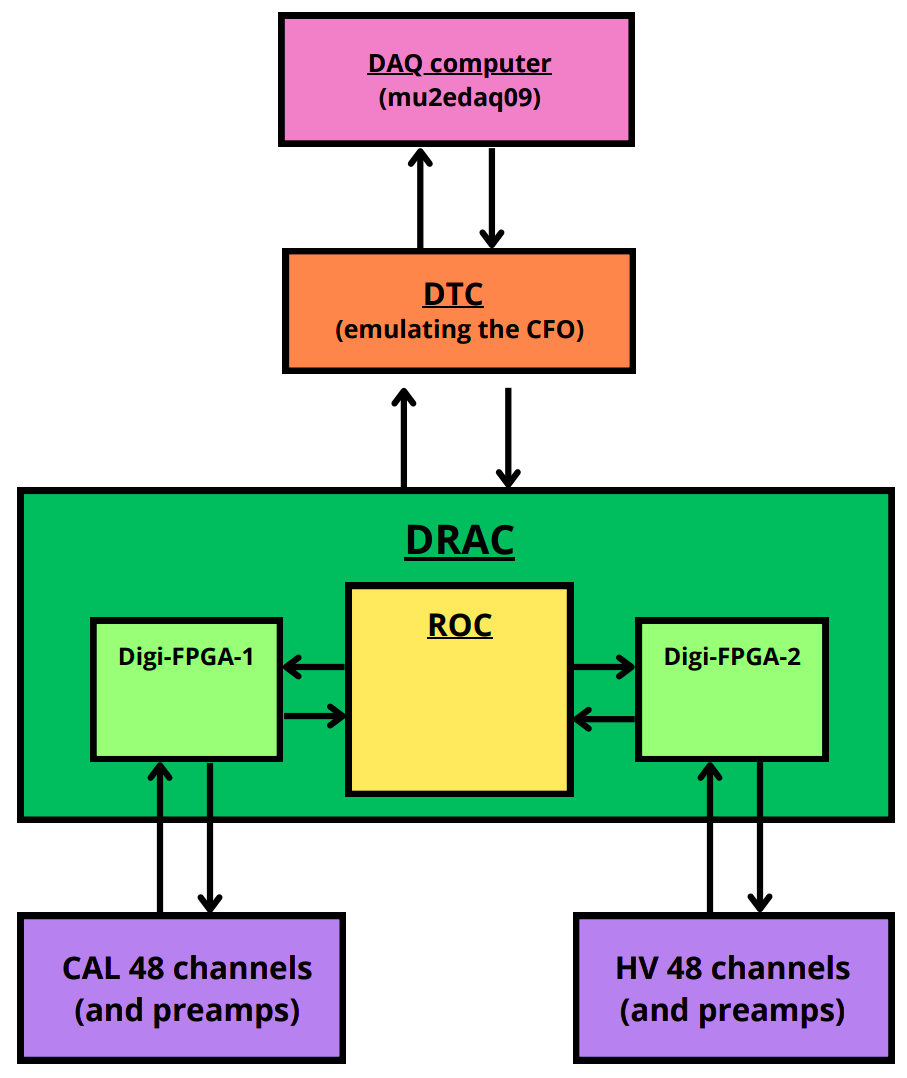
\includegraphics[width =0.5\textwidth]{figures/png/Screenshot_20240712_102528.png}
    \caption{Block diagram representation of the tracker DAQ test-stand. The two purple 
    blocks represent the two channel batteries (48 CAL channels on the left, 
    and 48 HV channels on the right), connected to their respective digi-FPGA 
    (light green boxes), located in the DRAC board (dark green box). The 
    digi-FPGAs are connected to the ROC (yellow box) that manages the communication with the
    DTC (orange box). The DTC is connected to the DAQ 
    computer (pink box - mu2edaq09).}
    \label{fig:blockdiagram}
    \end{figure}







  The test-stand includes the readout chain of an entire 96-channels tracker panel:  
  48 channels connected to the first digi-FPGA and 48 channels to the second one. 
  Each channel represents a tracker straw which was absent from our test stand.

  The DRAC board was connected via optical fiber to one DTC installed in DAQ computer (mu2edaq09).
  The DTC was programmed, for most of our tests, to emulate the CFO 
  functionality to send the request to the ROC to perform the readout of one event.
    The DTC emulated the CFO by sending a request 
    for one event, which was immediately followed by reading the event.


    Depending on the test to perform, it was possible to select one 
    between two ROC operating modes:
    \begin{itemize}
    \item  \textbf{ROC internal mode}: the ROC was emulating the data 
    itself (user-defined) without reading digi-FPGAs;
    \item  \textbf{ROC external mode}: the ROC receives data 
    from the digi-FPGAs. This will be the mode used during Mu2e data-taking.
    \end{itemize}
    For most of the tests performed, the ROC was operated 
    in the external mode: in some cases we simply used the 
    digi-FPGAs internal pulser, in some other cases we injected 
    calibration pulses directly in the CAL-side of the preamps at 
    a frequency we could customise.
    \begin{figure}[!h]
        \centering
        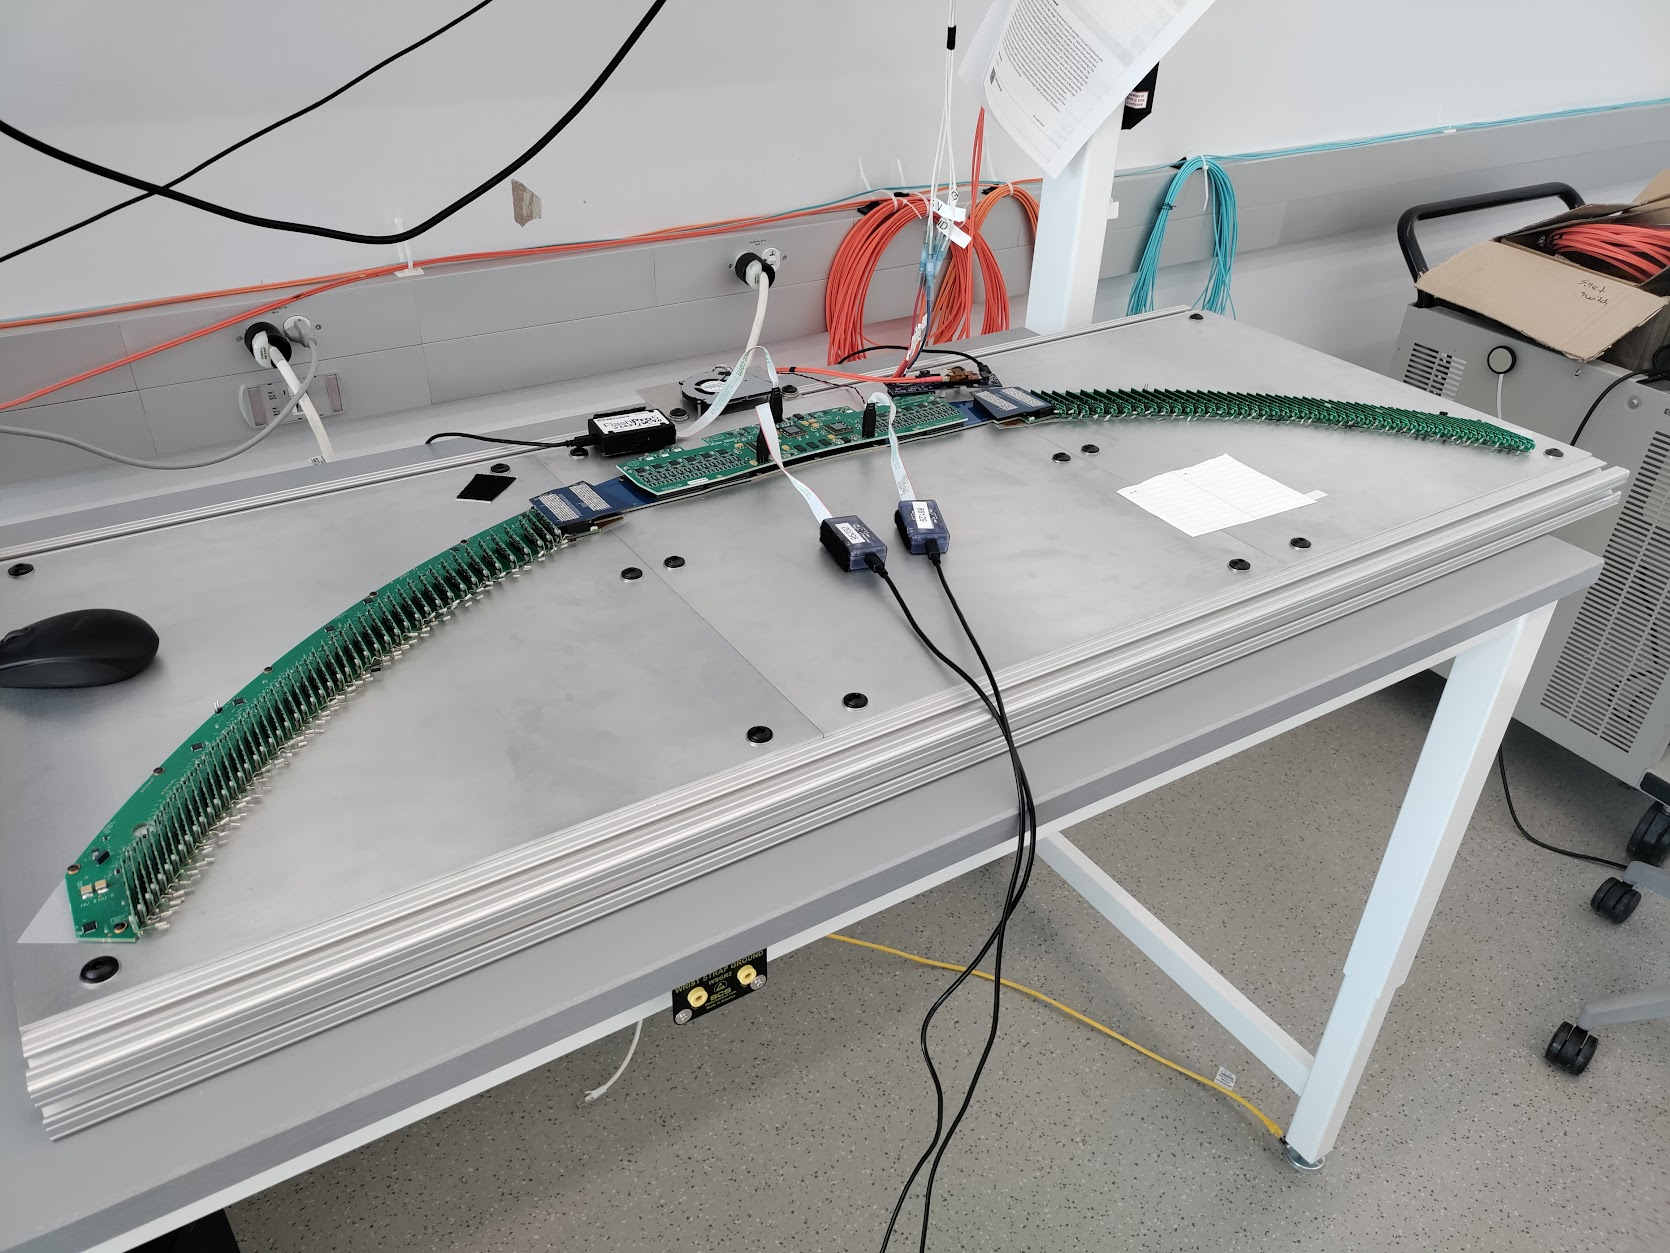
\includegraphics[width =0.6\textwidth]{figures/jpg/IMG_20240219_090538.jpg}
        \caption{The tracker DAQ test stand (TS1) installed at IERC facility 
        at Fermilab. The test-stand in the full readout chain 
        of one entire tracker panel: 48 channels on the HV-side 
        and 48 channels on the CAL-side, 1 DRAC board connected 
        via optical fiber to one DTC installed in the DAQ computer 
        (not shown).}
        \label{fig:TS1}
        \end{figure}
    Figure \ref{fig:timing} shows the timing diagram 
    for the readout of one detector channel.
    There are two important parameters: 
    the Event Window width ($T_{EW}$) shown in red, 
    that represents the distance between two consecutive 
    proton pulses (called heartbeats - HB's - separated by 
    $\sim$1.7 $\mu$s during Mu2e data taking), and 
    the separation $T_{gen}=1/f_{gen}$ between 
    two consecutive hits (represented by grey triangles), 
    where $f_{gen}$ is the generator frequency. 
    Each hit consists of two 16 bytes packets.

    For the purpose of these tests and DAQ commissioning, 
    the system allows for the flexibility to vary 
    the $T_{EW}$ between 700 ns to 50 
    $\mu$s. 

    The ROC firmware has an internal hit buffer 
    which stores up to 255 hits, which is adequate 
    given the expected hit multiplicity 
    in the detectors at run time. 
    Depending on $T_{gen}$ and $T_{EW}$, the data 
    taking can proceed in two different modes:
    \begin{itemize}
      \item \textbf{The ROC regular mode}: the total number of hits 
      within the event window is less than 255.
      In this case the ROC hit buffer doesn't get filled up 
      and the total number of 
      hits may vary from one event to another one. It is 
      expected that the number 
      of hits will not exceed the threshold of 255, 
      with an average of approximately 12 hits;
    \item \textbf{The ROC overflow mode}: the event window 
    is large enough, 
    so the total number of generated hits is 
      greater than 255. In this case
      the ROC hit buffer always gets filled up, and only 
      the first 255 hits are read out. 
      The hits readout after the first 255 are lost.
    \end{itemize}
   
    Since the timing of the readout (i.e. the Event Window) 
    is indipendent from the timing sequence 
    of the pulse generator, the number of pulses contained in 
    the Event Window can be different between two different 
    windows. 
    For example, Figure \ref{fig:timing} shows 
    that for two different relative timing offsets between 
    the Event Window and the sequence of generated pulses, 
    the number of pulses can be 
    either three (Figure \ref{fig:timing} Left) 
    or four (Figure \ref{fig:timing} Right).

    \begin{figure}[!h]
    \centering
    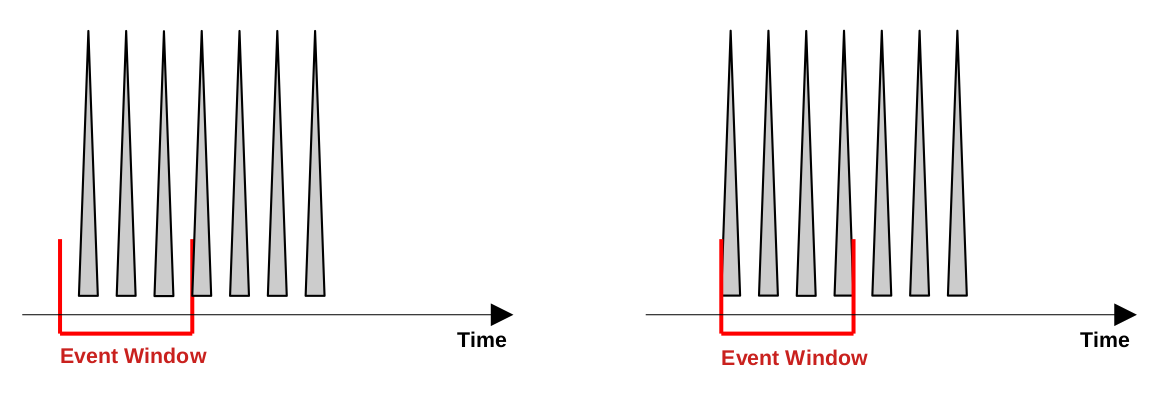
\includegraphics[width =1\textwidth]{figures/png/finalimg.png}
    \caption{Graphic illustration of pulses in an event window.}
    \label{fig:timing}
    \end{figure}

    The relative timing offsets among different channels of 
    the same digi-FPGA are of the order of few ns and can be 
    measured. The pulse sequences from the two digi-FPGAs are offset 
    relative to each other by a time interval $\Delta t$, which is 
    constant for as long as the DRAC board is 
    powered up and varies randomly between 0 and $T_{gen}$ 
    when DRAC is powercycled.


    Depending on the event window and the start of the pulse 
    sequence, the first channel in the read out sequence 
    reads out as many hits as allowed. Once all hits are read out, 
    the read out process for this channel 
    stops, and the process moves to the second one, 
    which then begins its own read out phase. This procedure 
    is repeated for all channels, following a fixed order.
\section{Validation of ROC read out and buffering}
The first test I performed has been to verify the correct performance of 
ROC buffering.
During these test, a single ROC was connected to the DTC. 
Data were collected with digi-FPGAs pulsed by their internal pulsers, 
with the ROC set in the external mode. 
Concering the digi-FPGAs pulse generators, they can operate at two specific frequencies, 
31.29 MHz/(2$^7$+1), or approximately 250 kHz, 
and 31.29 MHz/(2$^9$+1), or approximately 60 kHz.
        
\subsection{Development of the ROC bit-level simulation}\label{MonteCarlo}
 
ROC's digital readout logic allows to be 
emulated with a bit-level C++ simulation, 
which I contributed to develop. 
For each event, the simulated parameters 
are the number of hits in each channel and the total 
number of readout hits per event, which cannot exceed 255. 


The main steps of the simulation are the following ones:
\begin{itemize}
\item
  The start of the Event Window is set at $t=0$;
\item
  In each digi-FPGA, the timing of the first generated pulse 
  is randomly sampled from a uniform distribution between 0 and $T_{gen}$;
\item
Once the first pulse has been generated, the following pulses are 
added at the relative distance of $T_{gen}$,
  until the absolute time of the next pulse is above $T_{EW}$;
\item
  In the readout part of the simulation, 
  the pulses are readout following a predefined channel readout ordering;; 
\item
  the readout \textit{continues} until all the simulated hits 
  have been included, or the maximum threshold of 255 hits has been reached.
\end{itemize}
The simulation allows to introduce the offset between digi-FPGA-1 
and digi-FPGA-2 timing sequences and, 
internally to each digi-FPGA, the channel-to-channel 
offsets, as user-defined parameters.
To fine-tune the simulation, we measured the channel-to-channel 
offset from the data. For each digi-FPGA, we selected 
a reference channel
and measured the offset of the 
remaining 47 channels relative to it.
The reference channel is the first channel to 
be readout in each digi-FPGA: channel 91 for 
digi-FPGA-1 and 94 for digi-FPGA-2. 
Figure \ref{fig:delay1}(\ref{fig:delay2}) shows an example of 
distribution of the offset between the reference 
channel 91(94) and a randomly selected channel, 0(44) for 
digi-FPGA-1(digi-FPGA-2). 
The mean offset was determined with a simple 
Gaussian fit of the distribution. 
This procedure was repeated for all channels 
relative to each digi-FPGA.
All the measured offsets were of the order of a 
few ns and were inserted in the simulation because 
it was important to take into account all possible 
effects in the emulation of the ROC hit buffering 
to perform an accurate comparison between data and 
simulation, although we were aware of the fact that 
given the order of magnitude of these offsets, the 
impact was negligible.

  \begin{figure}[!h]
          \centering
      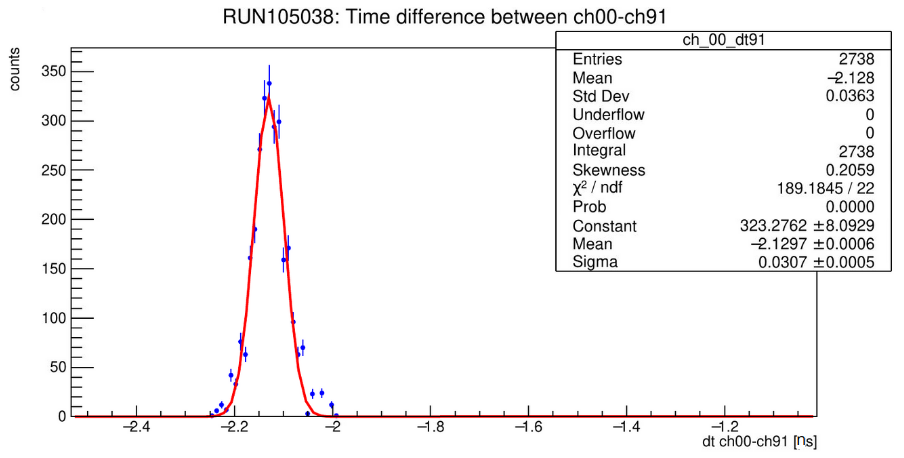
\includegraphics[width=0.75\textwidth]{figures/png/Screenshot from 2023-12-03 11-50-50.png}
      \caption{FPGA-1: histogram of the delay between 
      channel 0 and the reference channel 91, the first 
      to be readout.}
      \label{fig:delay1}
    \end{figure}
    \begin{figure}[!h]
          \centering
      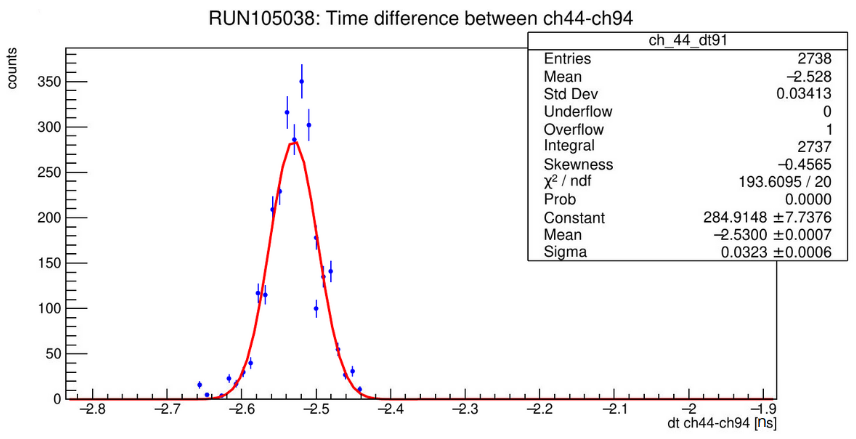
\includegraphics[width=0.75\textwidth]{figures/png/Screenshot from 2023-12-03 11-50-33.png}
      \caption{FPGA-2: histogram of the delay between 
      channel 44 and the reference channel 94, the first 
      to be readout.}
      \label{fig:delay2}
    \end{figure}
   
    The comparison between the data and the simulation 
    will be presented in the following sections, where 
    we will refer to $occupancy$ as the total number of hits 
    recorded in a given channel during the test run.
\subsection{The \textit{ROC buffer overflow} mode}
In the \textit{ROC buffer overflow} configuration (referred to 
as RUN281 in the following), 
the $T_{EW}$ was set to 50 $\mu$s and $f_{gen}$ to $\sim$60 kHz, 
which corresponds to 
a time distance between two consecutive pulses of 
approximately 16 $\mu$s.
This implies that the number of hits in a 
readout window could be 
either 3 or 4, depending on the offset 
between the readout window and the generated pulses sequence.
\subsubsection{Hit timing and occupancy}\label{over}
We first checked the distribution of the hit time for 
each readout channel, and the distribution of the 
total number of hits (occupancy) in one specific 
readout channel as a function of the channel number. 
Figure \ref{fig:1} shows the hit time 
distributions for two selected channels, 
channel 0 of digi-FPGA-1 and channel 2 of digi-FPGA-2.
The top distribution is, as expected, uniform, 
however the bottom one shows some unexpected features.
\begin{figure}[!h]
  \begin{subfigure}[b]{\textwidth}
      \centering
      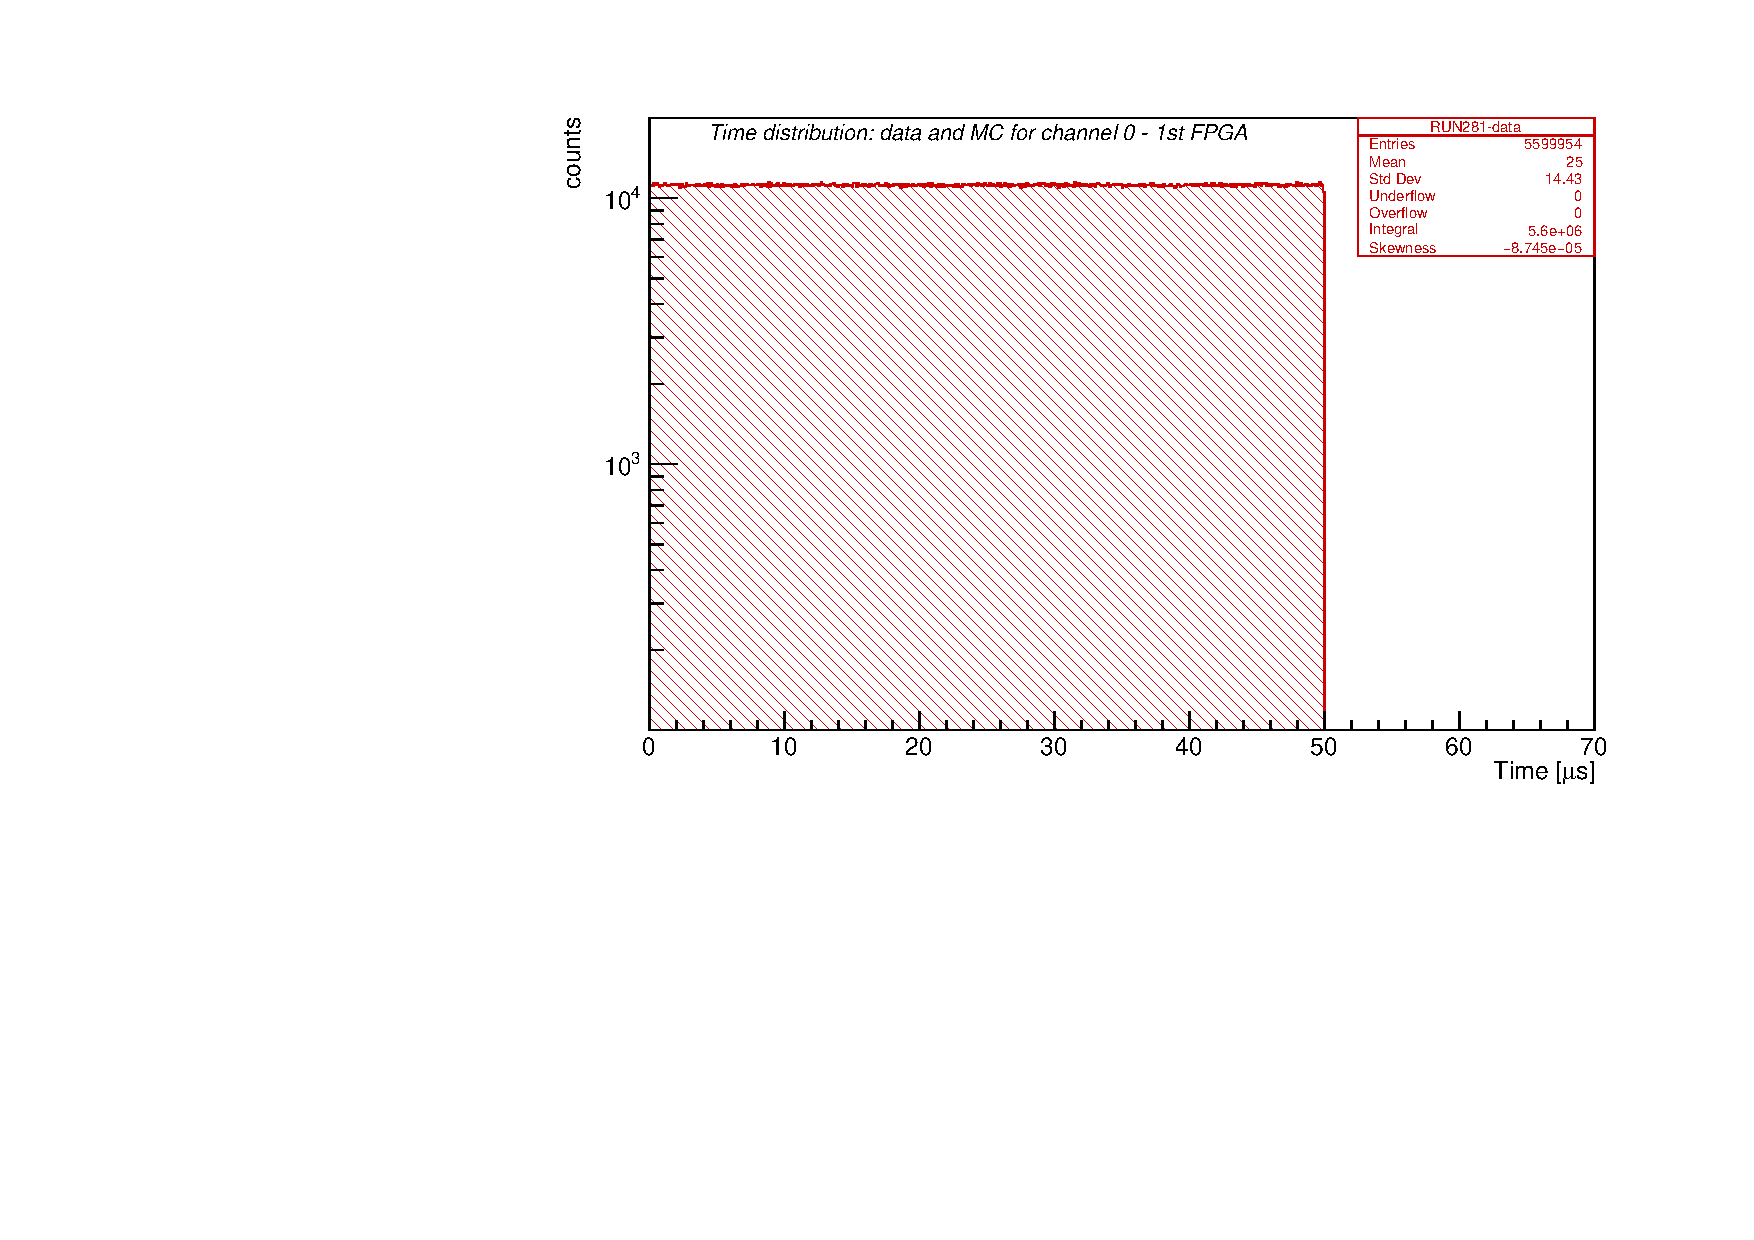
\includegraphics[width=0.7\textwidth]{figures/pdf/figure_00007_timedistr_roc_simulation_ch0_281.pdf}
      \label{fig:t1}
  \end{subfigure}
\\
  \begin{subfigure}[b]{\textwidth}
      \centering
      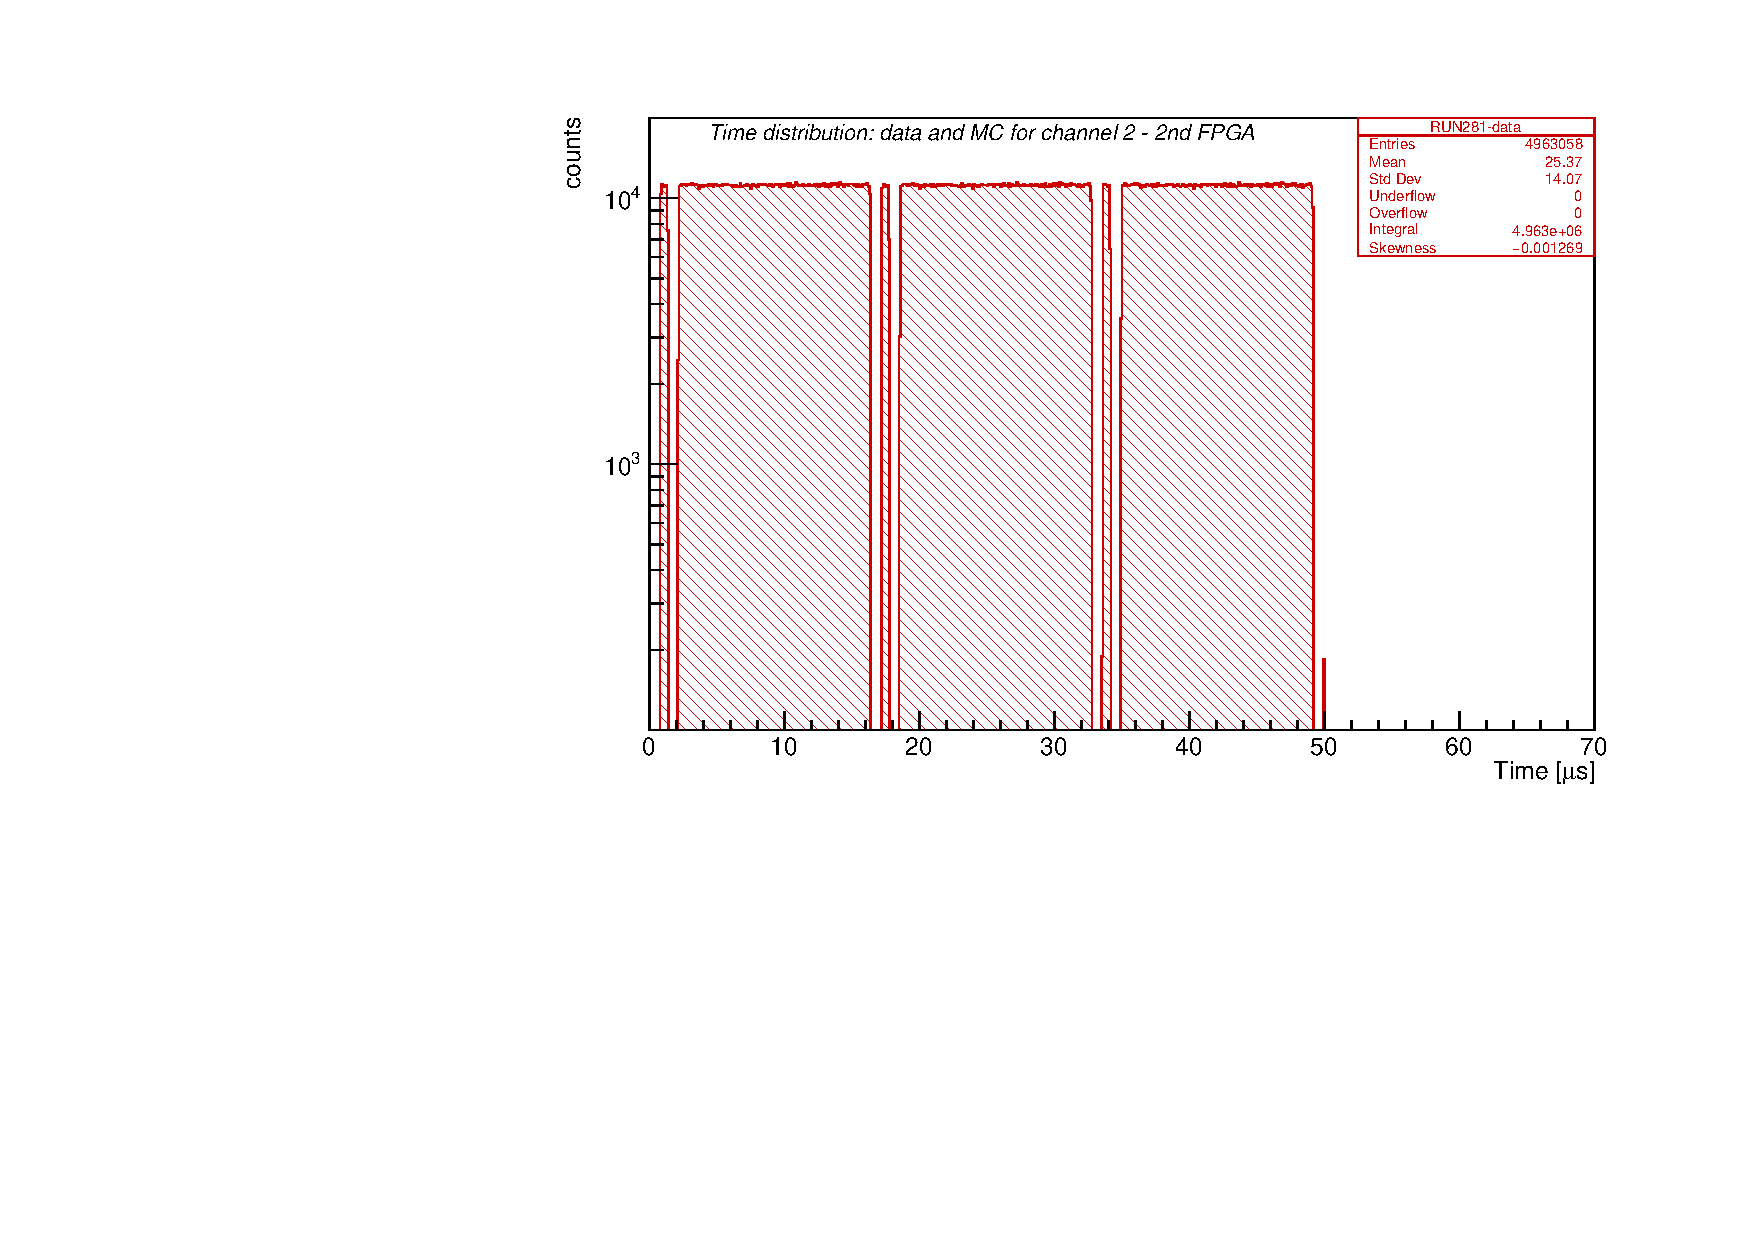
\includegraphics[width=0.7\textwidth]{figures/pdf/figure_00003_timedistr_roc_simulation_ch2_281.pdf}
      \label{fig:t2}
  \end{subfigure}
     \caption{(Top): time distribution of hits in the channel 0 in the digi-FPGA-1.
     (Bottom): time distribution of hits in the channel 2 in the digi-FPGA-2.}
     \label{fig:1}
\end{figure}
The explanation for the two different distributions 
can be found from Figure \ref{fig:2} (Top), 
which shows the occupancy as a function of channel number 
(red is for data, blue for simulation).

The ordering of the bins in the histogram corresponds 
to the channel readout ordering: this means that 
the first bin on the left corresponds to the first 
readout channel and the last one on the right 
corresponds to the last readout channel.
In other words, channels on the left 
are at the beginning of the readout sequence 
and are, in these conditions, always 
completely readout. On the other hand, channels on 
the right are in the 
later part of the readout sequence and may 
not have all the hits readout, 
since the ROC buffer may be in overflow.
  \begin{figure}[!h]
    \begin{subfigure}[b]{\textwidth}
        \centering
        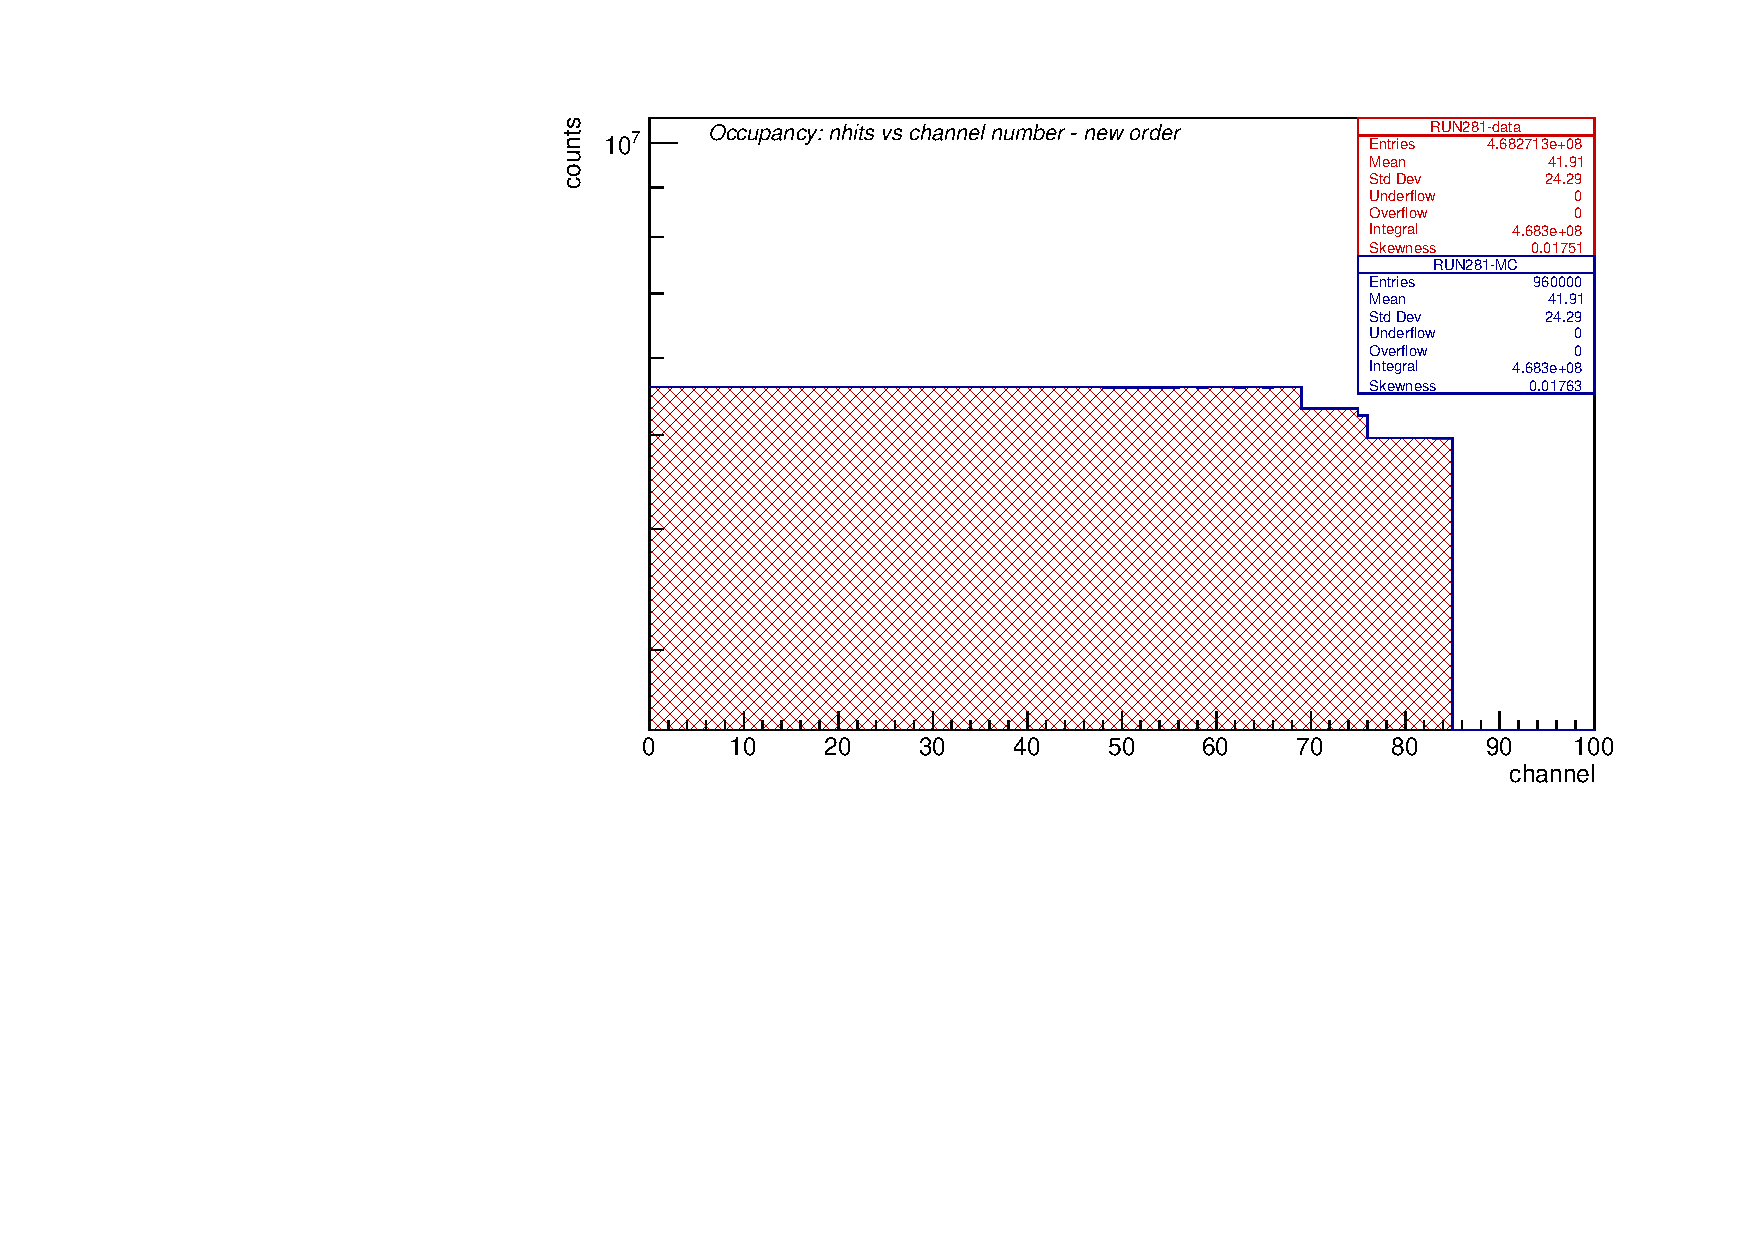
\includegraphics[width=0.7\textwidth]{figures/pdf/figure_00004_nhitsvschannel_roc_simulation_281.pdf}
        \label{fig:tt1}
    \end{subfigure}
  \\
    \begin{subfigure}[b]{\textwidth}
        \centering
        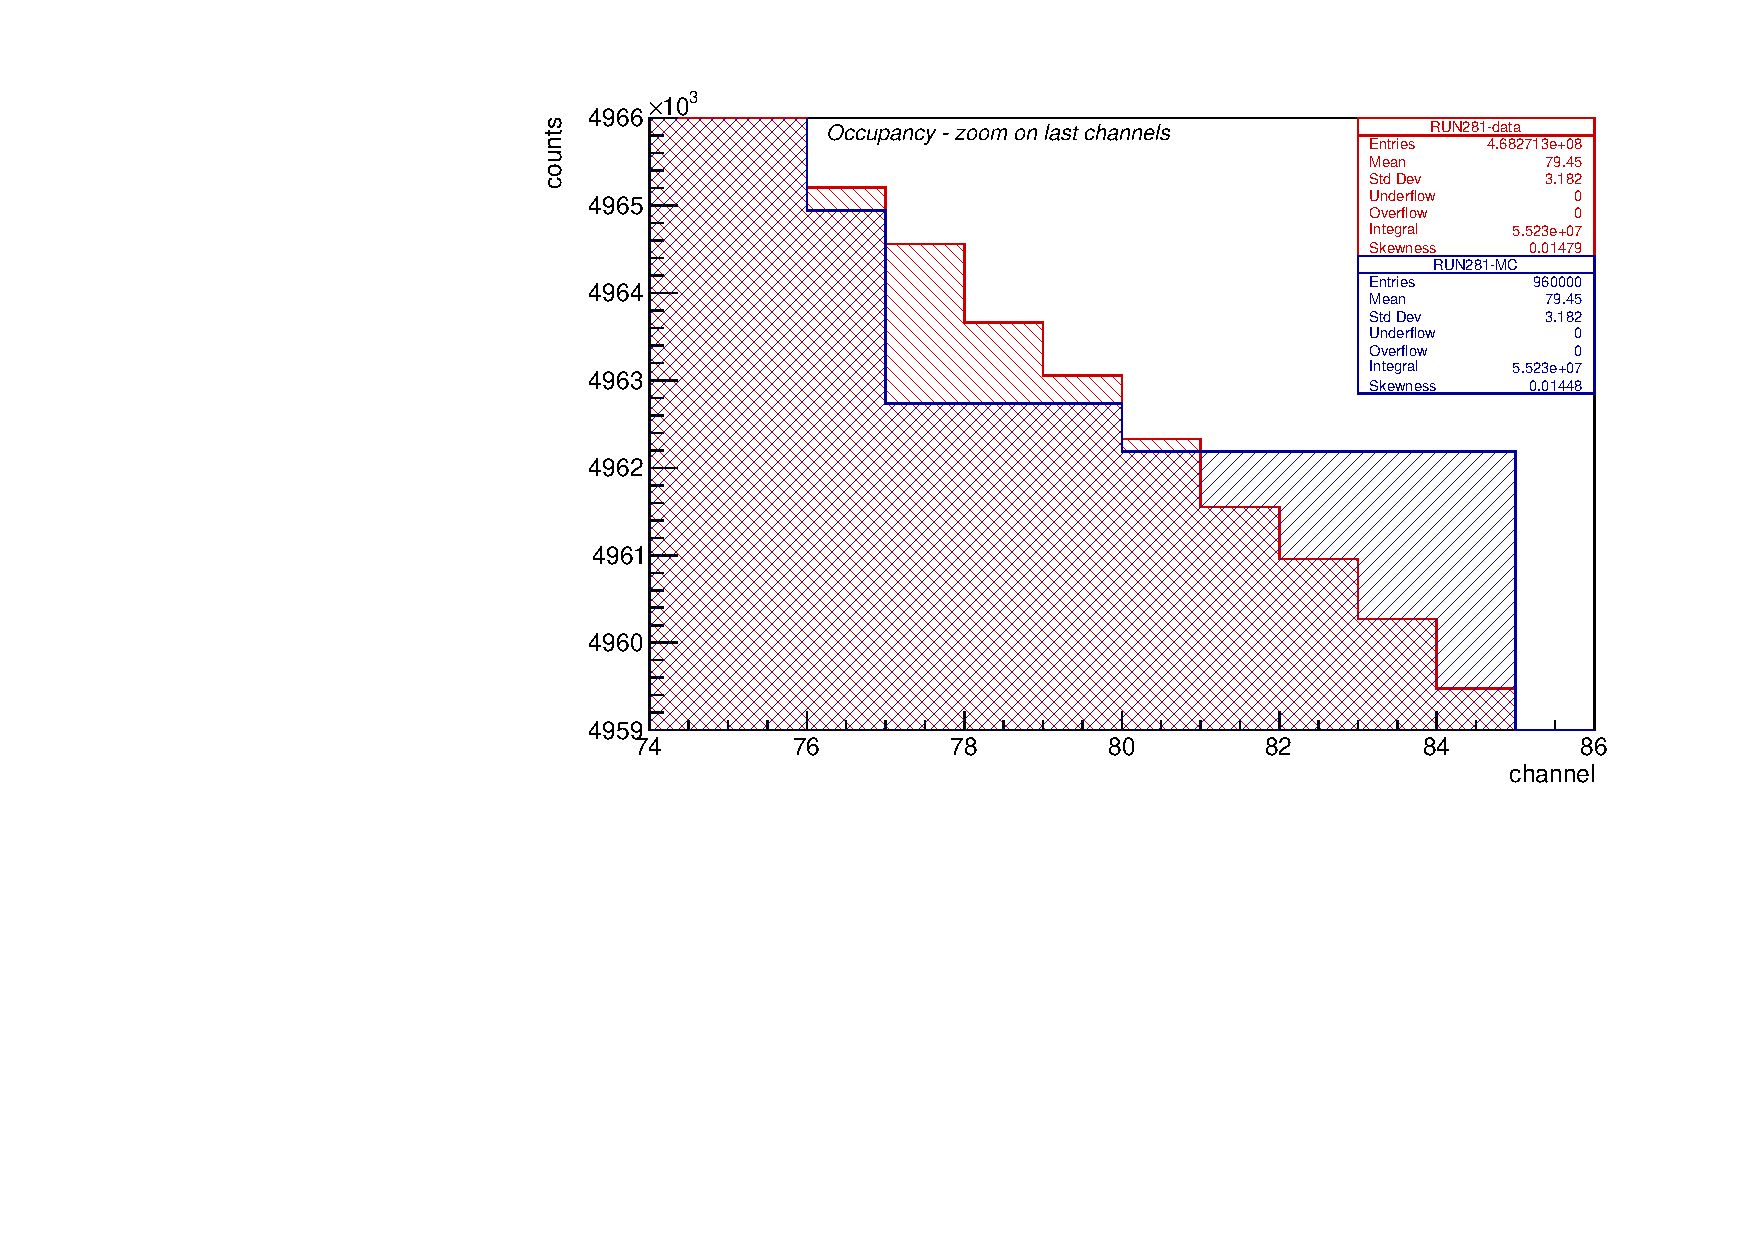
\includegraphics[width=0.7\textwidth]{figures/pdf/figure_00014_nhitsvschannel_roc_simulation_281.pdf}
        \label{fig:tt2}
    \end{subfigure}
       \caption{(Top): number of hits versus the channel number 
       (data in red, Monte Carlo in blue). The two distributions 
       are normalized to the same number of events.
       The channels are numbered in the readout order. Not all 96 channels 
       are present in the histogram 
       because the maximum threshold of 255 hits was reached with fewer channels.
       (Bottom): zoom on the last channels in the readout sequence. The data 
       and MC distributions differ from each other by $\sim$ 10$^{-3}$.}
       \label{fig:2}
  \end{figure}


Figure \ref{fig:66} shows the distribution of the number of 
hits of channel 0 of digi-FPGA-1. As expected, 
the majority of events 
has 3 hits, with a tail of 4 hits. 
This provides an explanation for Figure \ref{fig:2} (Top).
\begin{figure}[!h]
\centering
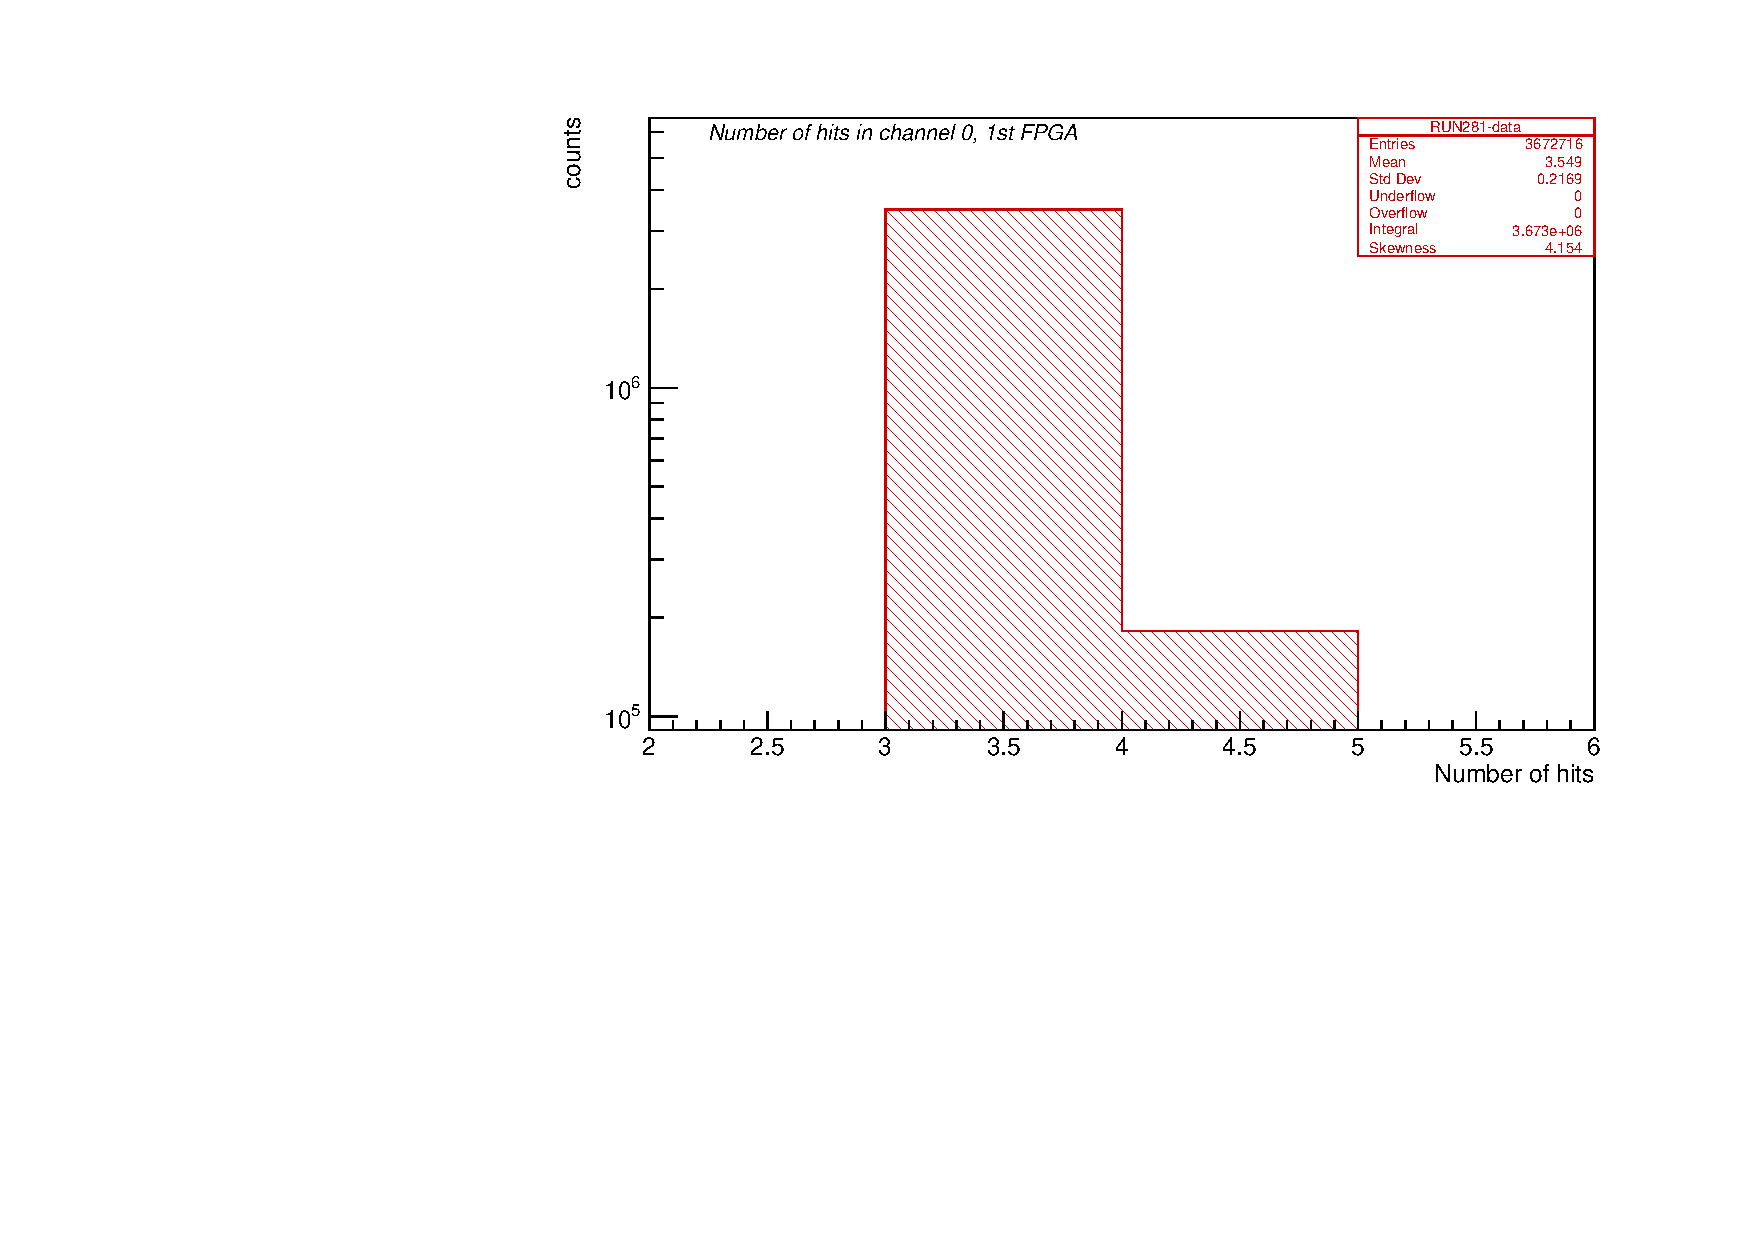
\includegraphics[width =0.7\textwidth]{figures/pdf/figure_00066_nhits_ch00_run281.pdf}
\caption{
  The distribution of the number of hits in the channel 
  0 of the first digi-FPGA (RUN281).
}
\label{fig:66}
\end{figure}
The first 69 bins of the histogram (Figure \ref{fig:2} (Top)) 
show a flat distribution with the maximum observed occupancy. 
Additionally, there are two more plateaus with slightly lower 
occupancy (less than 10\% lower): one over the following 
7 bins (with a small $dent$ at the end), and the other 
spanning the last 9 bins.
This pattern can be generated by adding together the 
following three types of events.
\begin{itemize}
  \item \textbf{0-68th read out channels}: 
  the 48 channels of the digi-FPGA-1, the first one to be readout, 
  are those with 4 hits per channel, 
  which makes a total of 192 hits stored in the ROC buffer. 
  In these conditions, 63 hits can still be stored.
  Because of the delay between the first and second digi-FPGA, 
  only three hits can be read out by each channel 
  of the second digi-FPGA. The first 21 channels of the second 
  digi-FPGA will be those with 3 hits per channel, resulting in a 
  total of 255 hits. All the hits sent to the following 
  channels are lost.
  \item \textbf{0-75th read out channels}: 
  the 48 channels of the first digi-FPGA are 
  those with 3 hits per channel, 
  which makes a total of 144 hits stored in the ROC buffer.
  The \textit{dent} at the end of the second 
  plateau is due to the 
  fact that the digi-FPGA-2 contributes 111 hits and this number 
  is not an integer of 4. 
  The first 27 channels of the digi-FPGA-2 contribute
  4 hits per channel each, but 
  the three hits from channel 28 in the 
  readout sequence
  fill up the total ROC buffer of 255 hits. 
  \item \textbf{0-85th read out channels}: 
  the 48 channels of the first digi-FPGA and the 
  first 37 channels to be read out in the digi-FPGA-2 
  are those with 3 hits, 255 hits in total.

\end{itemize}
Not all 96 channels are present in the 
histogram because the maximum 
threshold of 255 hits was reached with 
fewer channels, in particular the number of 
85 read out channels corresponds to the 
sum of 48 read out channels in the first 
digi-FPGA and 37 read out channel in the second digi-FPGA.


Figure \ref{fig:2} (Bottom) shows a zoom on the 
rightmost channels of the distribution.
The relative difference between the data and 
the MC distributions 
is at a level of $10^{-3}$, which is a 
very good agreement.


Coming back to Figure \ref{fig:1}, the first 
channels in the readout sequence
always have all their hits read out,
while the channels in the end of the readout sequence do not,
as the ROC hit buffer gets filled up after
the first 255 hits are read out.
This results in a uniform time distribution 
for the first channels readout and in a non-uniform
time distribution for the last readout channels, 
depending on $T_{gen}$ and $T_{EW}$.
The dips in the hit timing distribution for 
channel 2 are defined by the timing offset
between the two digi-FPGA pulsers. 


%%%%%%%%%%%%%%%%%%%%%%%%%%%%%%%%%%%%%%%%%%%%%%%%%%%%%%%%%%%%%%%%%%%%%%%%%%%%%%
\subsubsection{Number of hits}
Figure \ref{fig:3} shows that in the \textit{buffer overflow} mode all events,
as expected, have 255 hits read out per event.

\begin{figure}[!h]
\centering
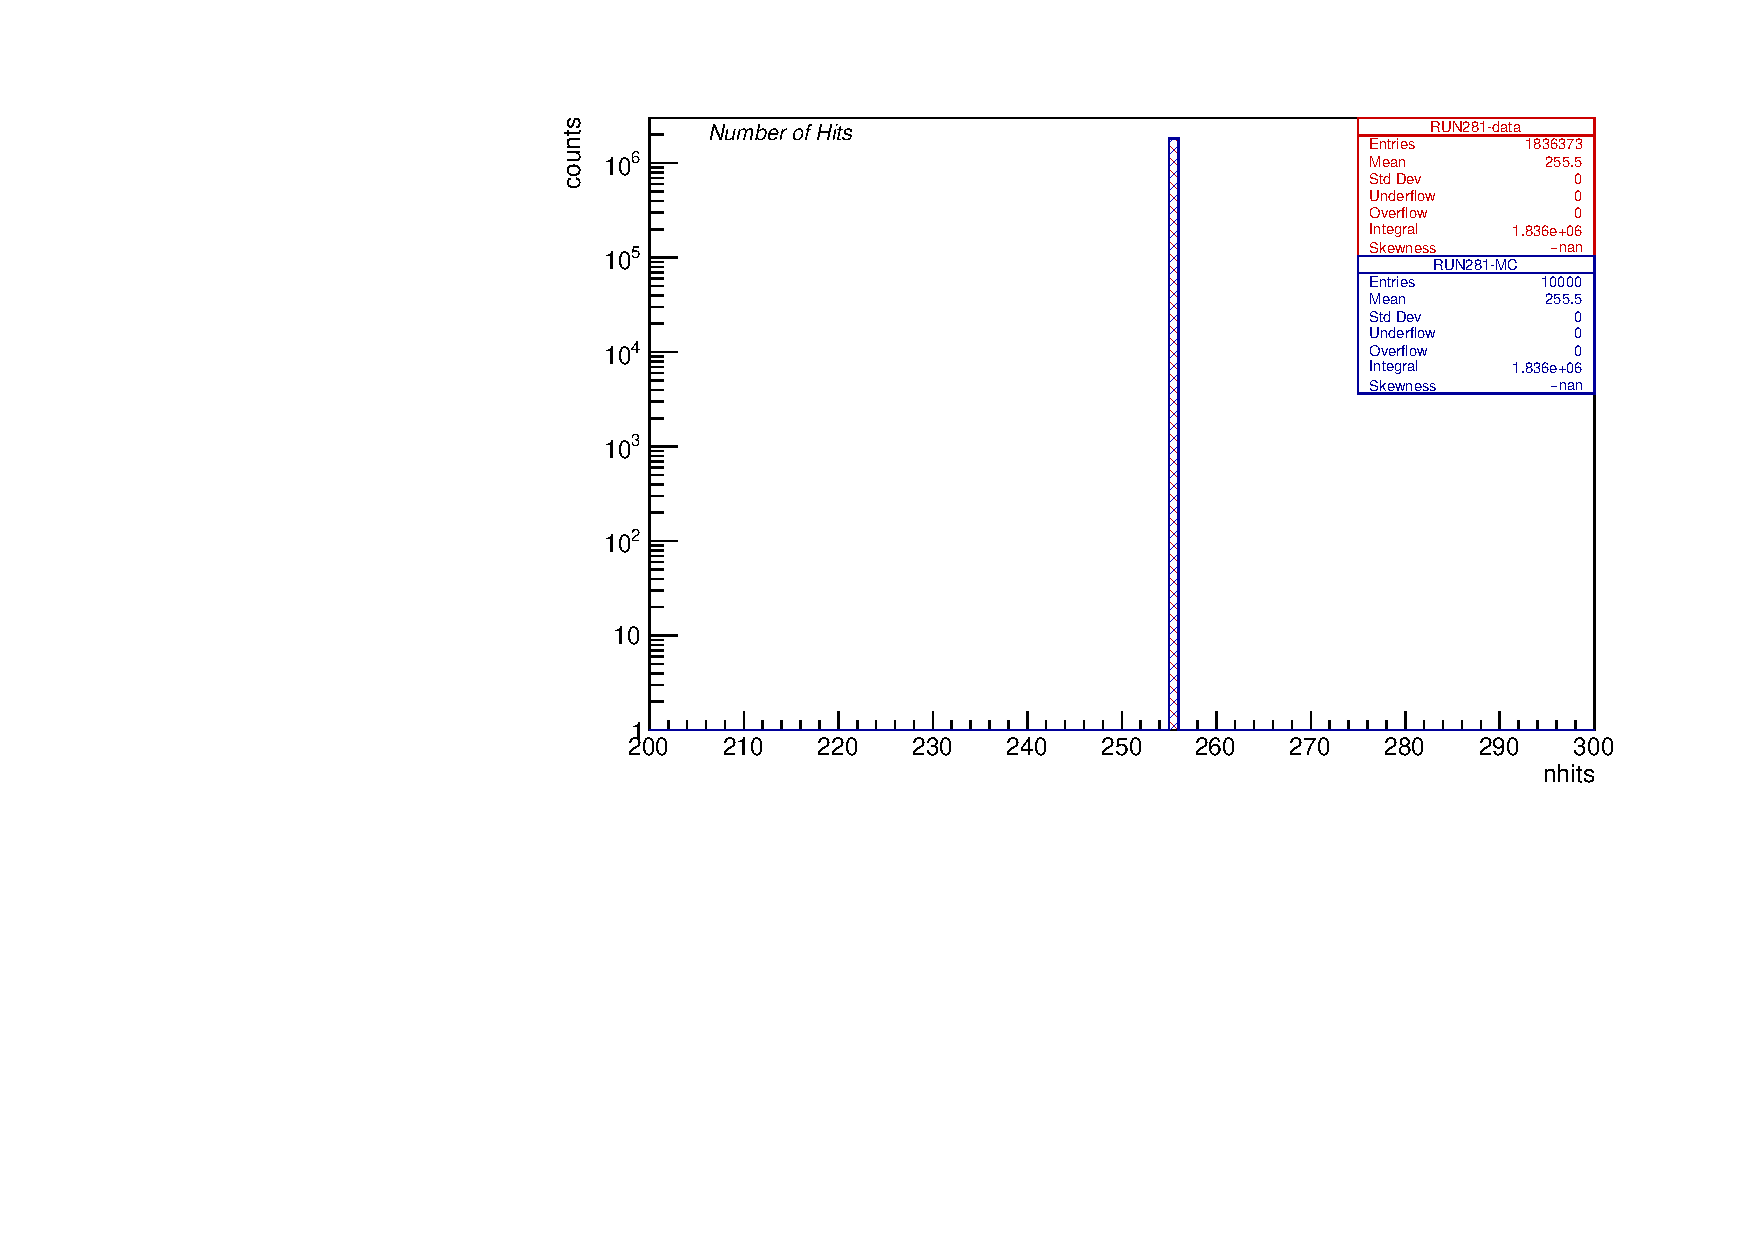
\includegraphics[width =0.7\textwidth]{figures/pdf/figure_00008_nhits_281.pdf}
\caption{
  The distribution of the total number of hits read out per event. 
  (data in red, Monte Carlo in blue). The two distributions 
  are normalized to the same number of events.
}
\label{fig:3}
\end{figure}
\subsection{The \textit{ROC buffer regular} mode }
In the \textit{regular} configuration, which will be referred to as RUN105038, the event window size is 25 $\mu$s
and the pulser rate is 60 kHz.

\subsubsection{Time distribution and occupancy}

Similar to Section \ref{over}, Figure \ref{fig:4} shows the distributions
of the number of hits in two channels, one from the 
FPGA-1 and another one, from the digi-FPGA-2. 
In this readout configuration, the expected number of pulses in a given channel
within the event window is one or two, and the total number of pulses is always below 255.

\begin{figure}[!h]
  \begin{subfigure}[b]{\textwidth}
      \centering
      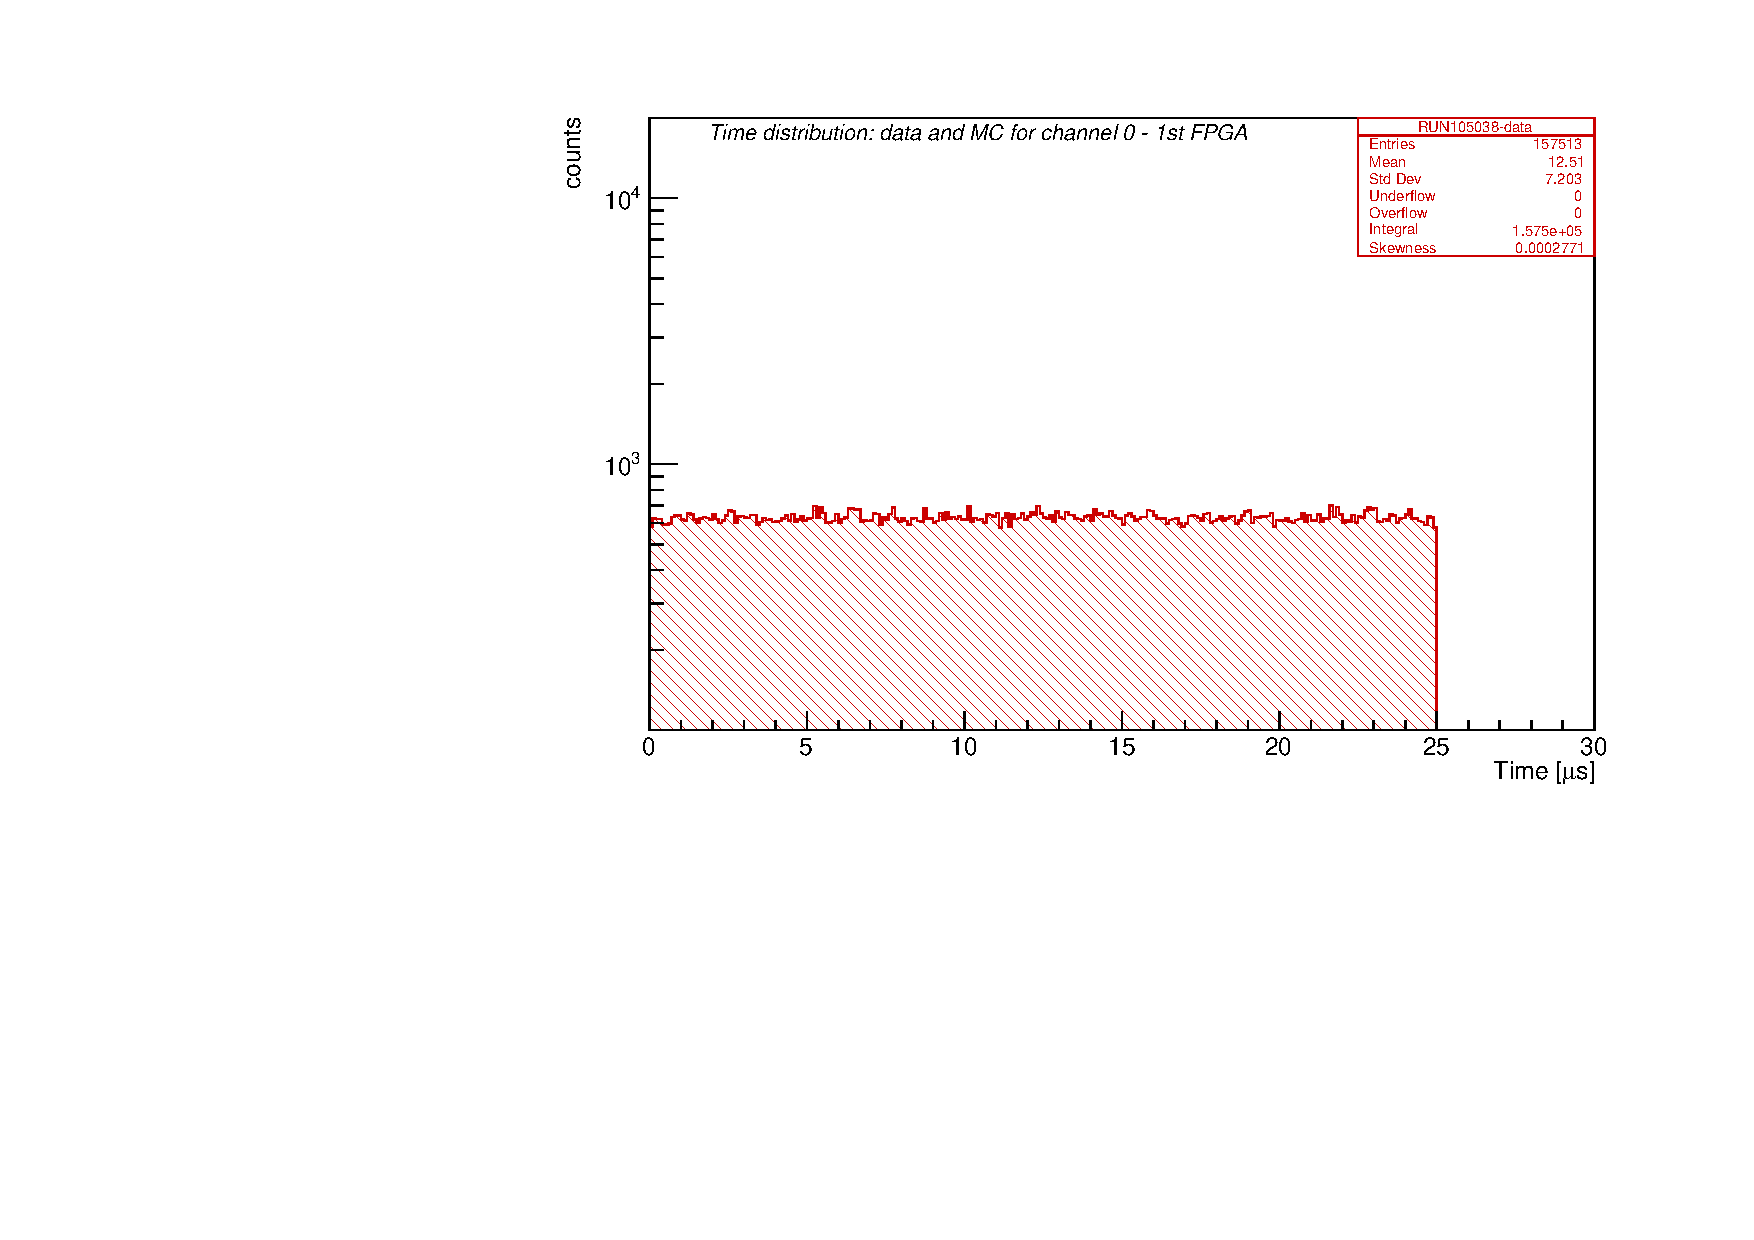
\includegraphics[width=0.7\textwidth]{figures/pdf/figure_00001_timedistr_roc_simulation_10538.pdf}
      \label{fig:ttt1}
  \end{subfigure}
\\
  \begin{subfigure}[b]{\textwidth}
      \centering
      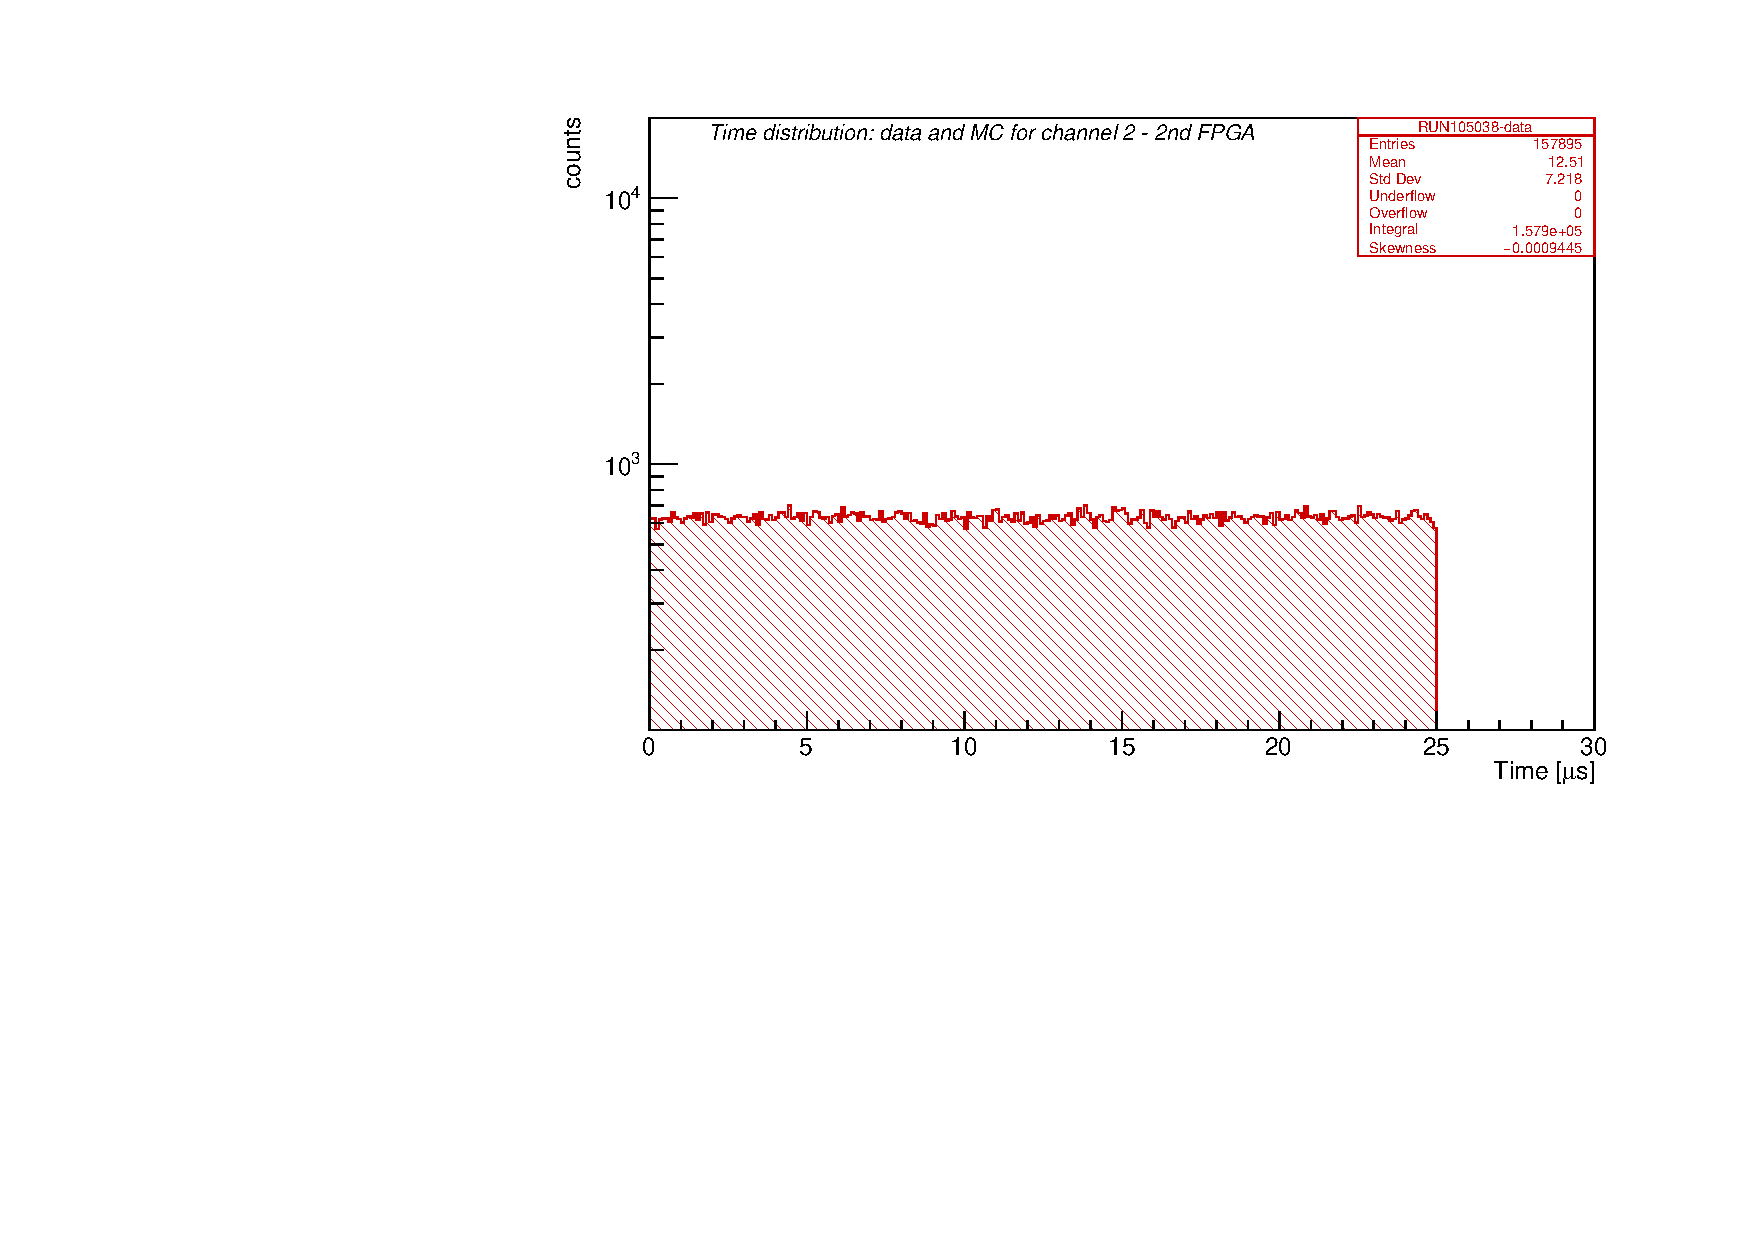
\includegraphics[width=0.7\textwidth]{figures/pdf/figure_00012_timedistr_roc_simulation_ch2_105038.pdf}
      \label{fig:ttt2}
  \end{subfigure}
     \caption{(Top): the hit time distribution for this in channel 2, the digi-FPGA-2. 
     (Bottom): the hit time distribution for hits in channel 0, the digi-FPGA-1.}
     \label{fig:4}
\end{figure}

In this mode, the readout of a given channel is not affected by the readout of previous
channels and the \textit{occupancy} distributions shown in Figure \ref{fig:5} are, as expected, uniform.
\begin{figure}[!h]
\centering
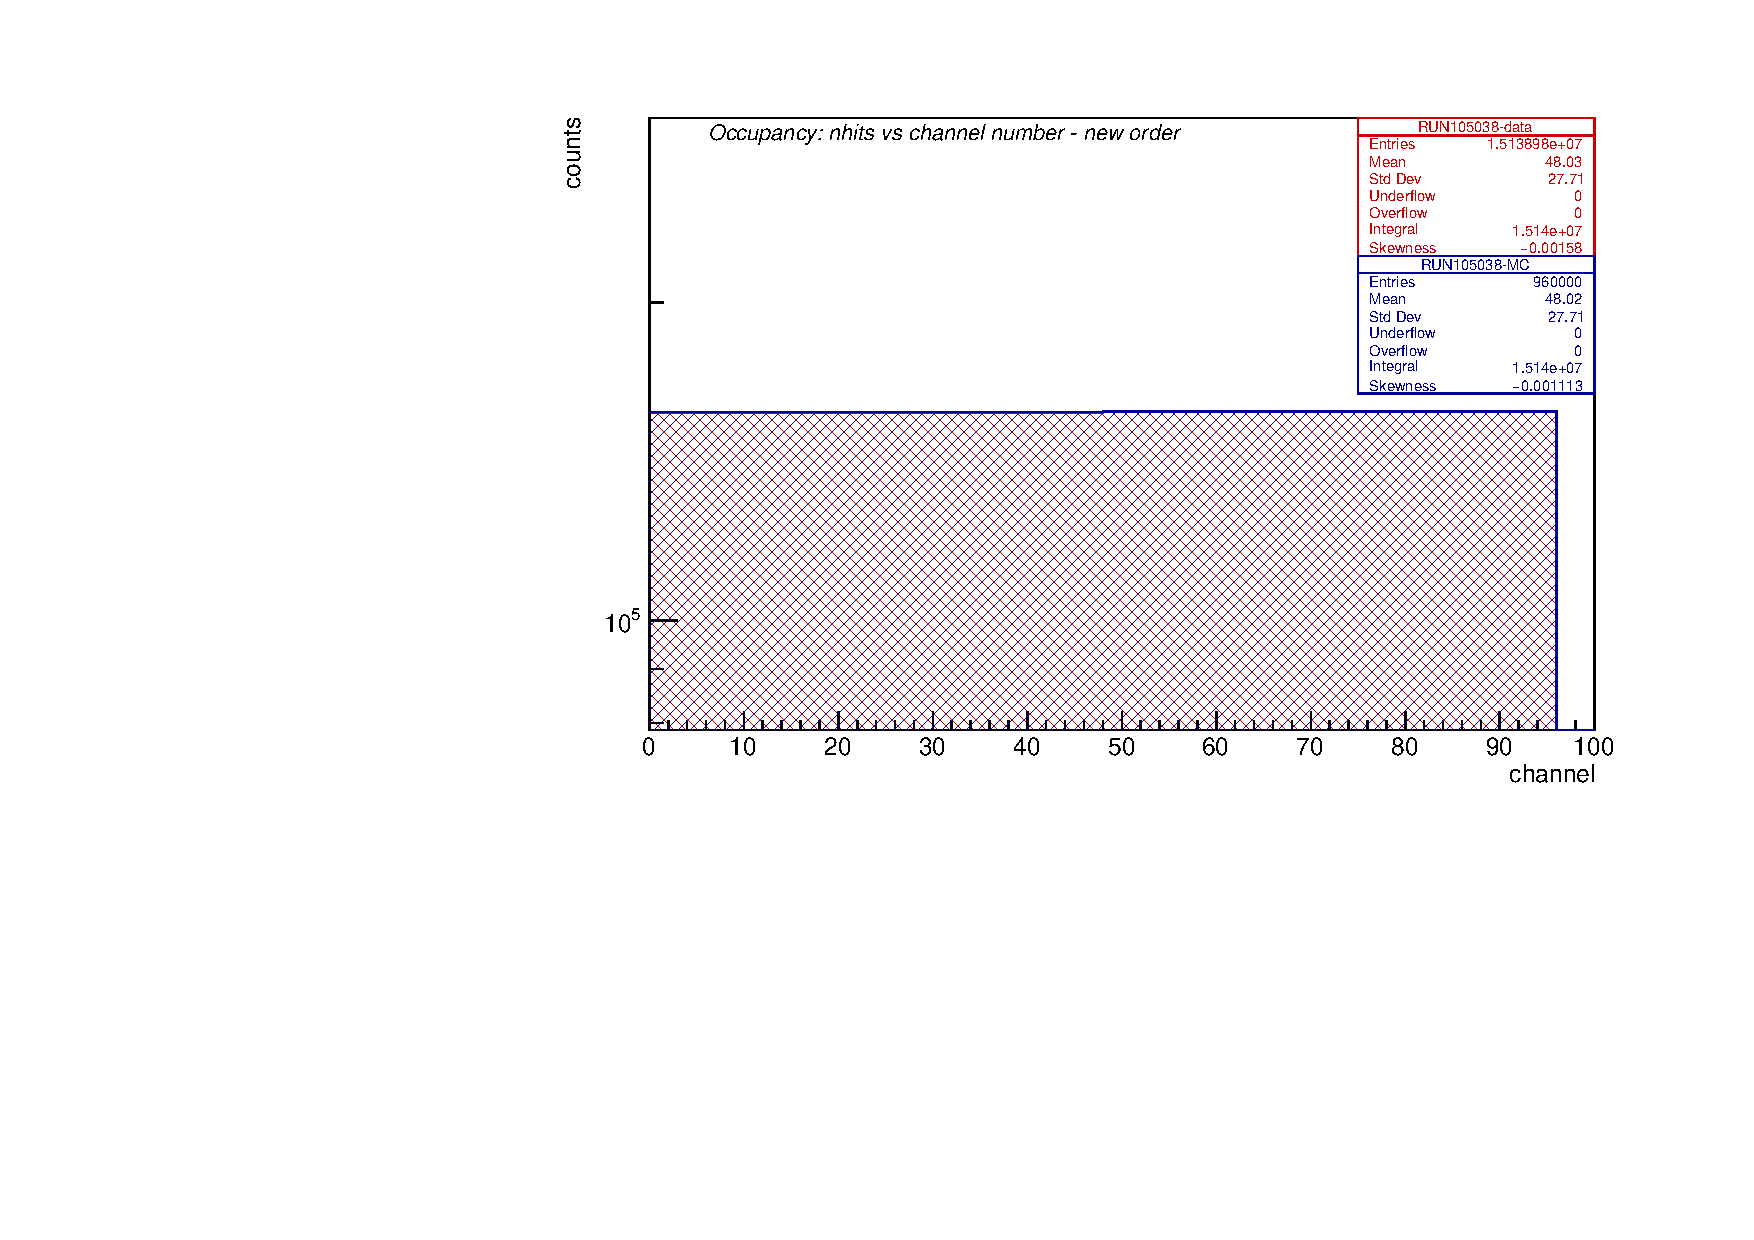
\includegraphics[width =0.7\textwidth]{figures/pdf/figure_00002_nhitsvschannel_roc_simulation_2.pdf}
\caption{The number of hits versus the channel number for RUN105038 
(data in red, Monte Carlo in blue). The two distributions 
are normalized to the same number of events. All 96 channels are read out.}
\label{fig:5}
\end{figure}


Figure \ref{fig:67} shows the distribution of the number of hits in the channel 0 (FPGA-1).
\begin{figure}[!h]
\centering
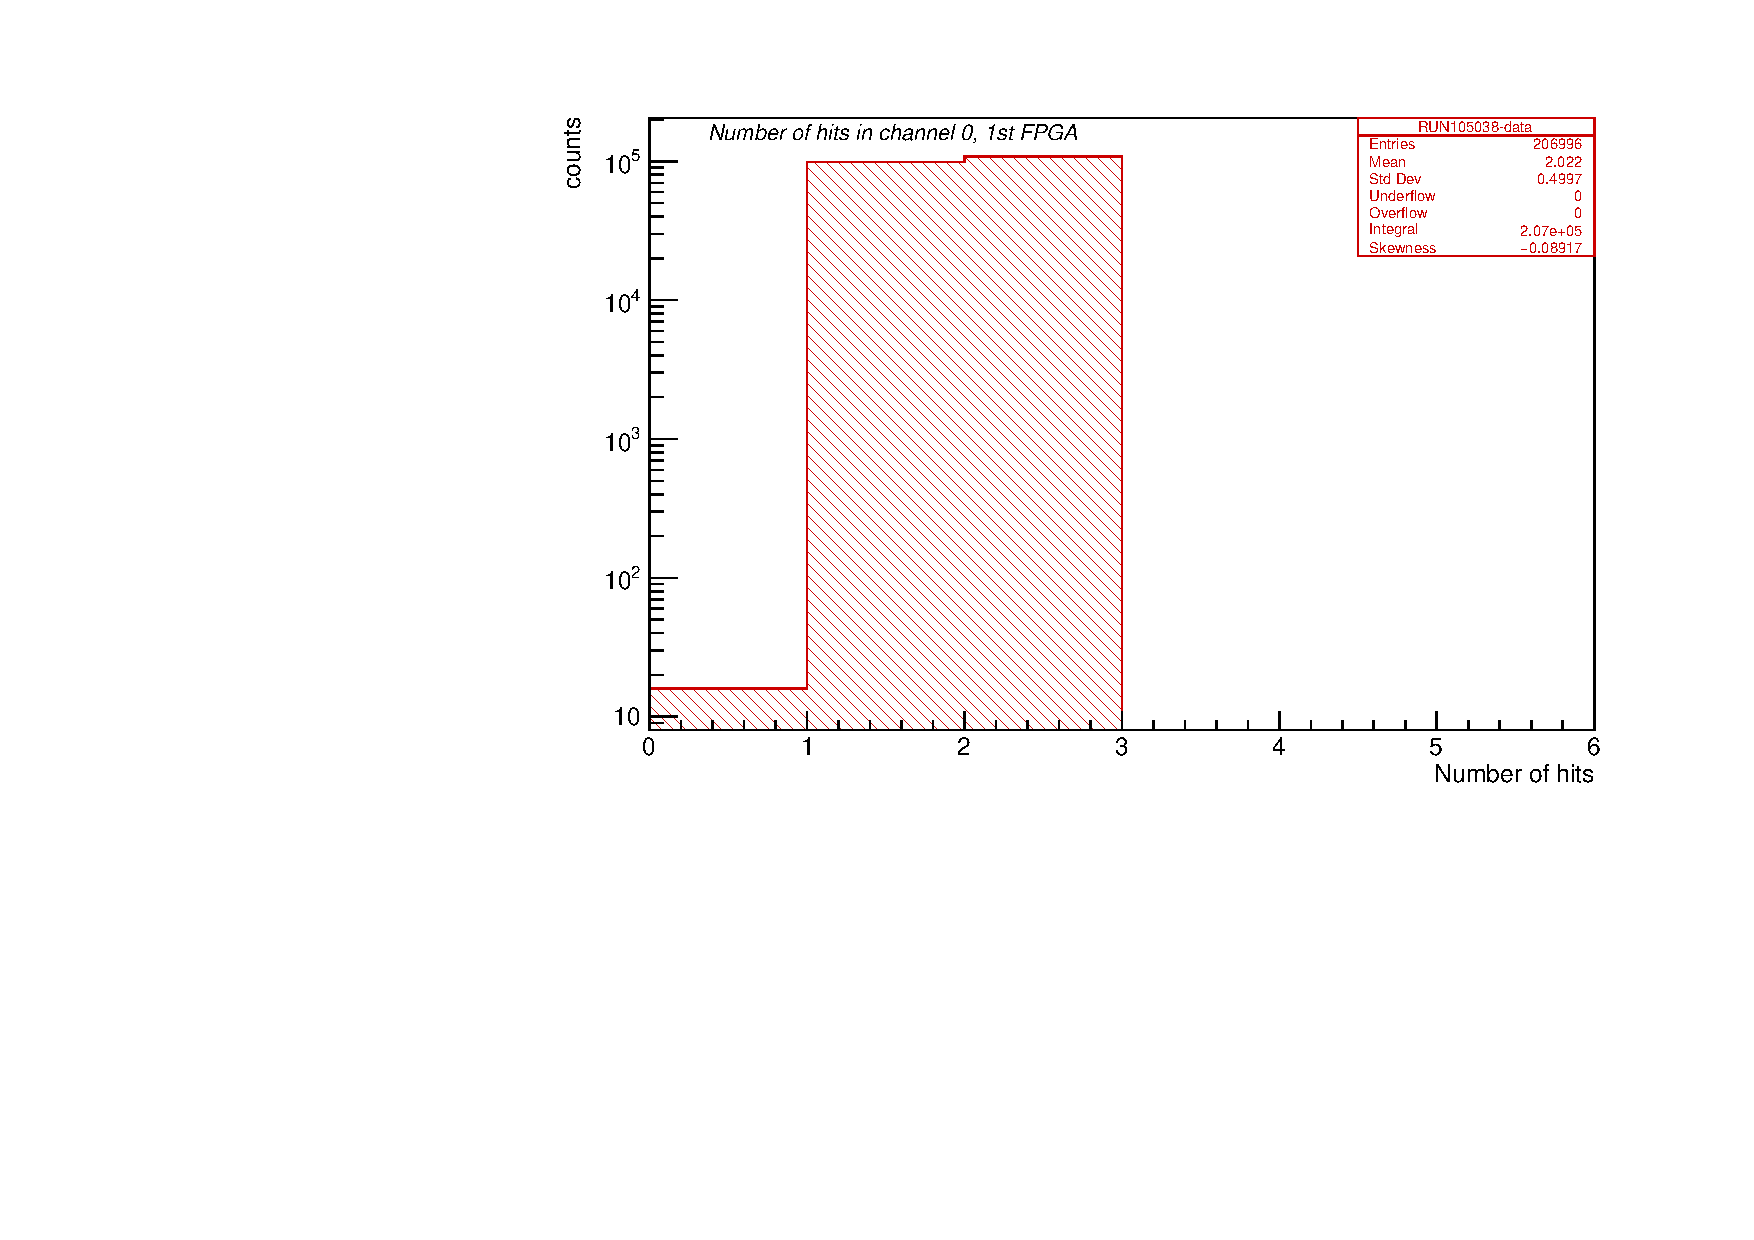
\includegraphics[width =0.7\textwidth]{figures/pdf/figure_00067_nhits_ch00_run105038.pdf}
\caption{
  The distribution of the number of hits in channel 0, digi-FPGA-1, for RUN105038.
  Entries in the $n$(hits)=0 bin are due to the readout errors.
}
\label{fig:67}
\end{figure}

%%%%%%%%%%%%%%%%%%%%%%%%%%%%%%%%%%%%%%%%%%%%%%%%%%%%%%%%%%%%%%%%%%%%%%%%%%%%%%
\subsubsection{Number of hits}
Compared to RUN281, the event window in RUN105038 was twice shorter
and the ROC readout buffer wasn't getting filled up.
The total number of hits within the event window depends on the relative offset
of the event window with respect to the digi-FPGA pulsers, and varies from
144 to 192, as shown in Figure \ref{fig:6}.

\begin{figure}[!h]
\centering
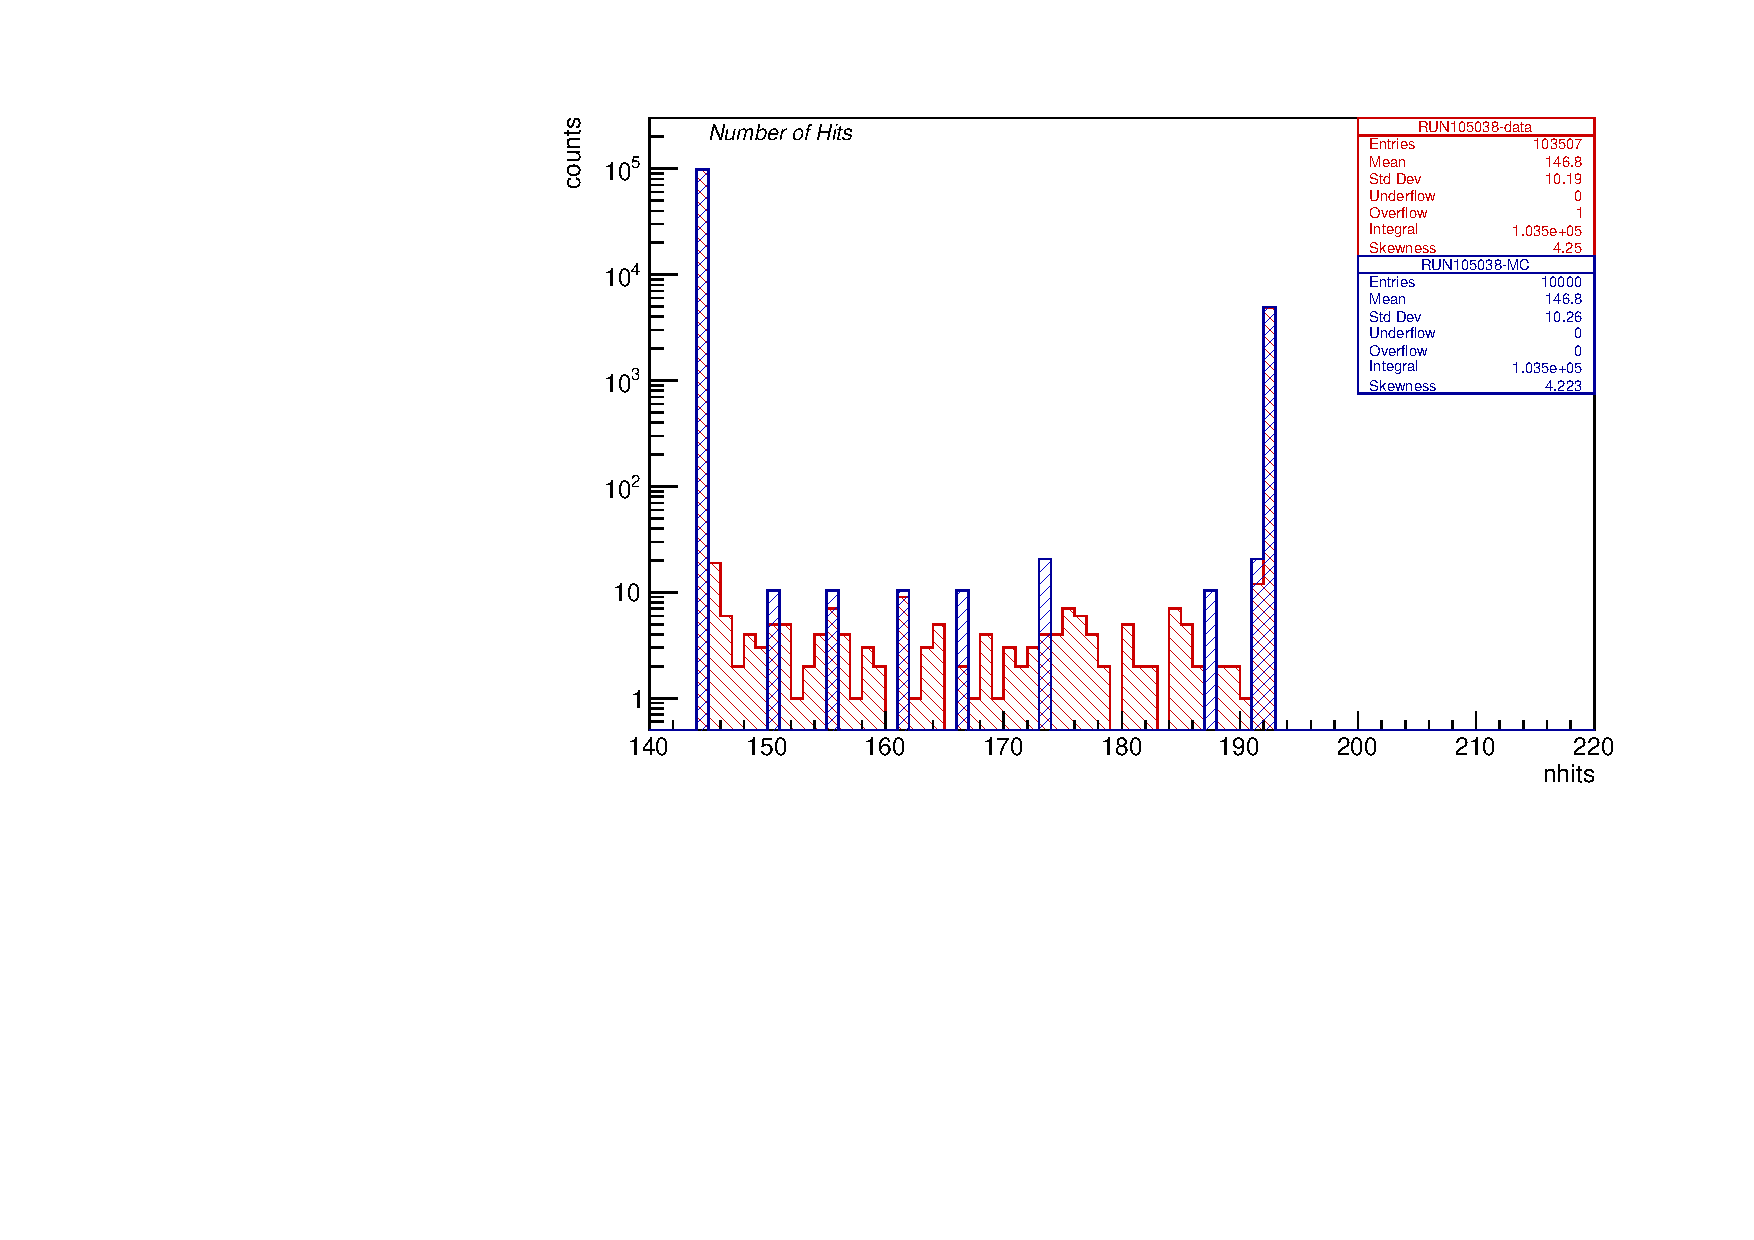
\includegraphics[width =0.7\textwidth]{figures/pdf/figure_00009_nhits_105038.pdf}
\caption{
  The distribution of the total number of hits per event in \textit{non-saturated} mode 
  (data in red, Monte Carlo in blue). The two distributions 
  are normalized to the same number of events.
}
\label{fig:6}
\end{figure}


\section{Primitive Data Quality Monitoring}\label{dqm}
The goal of this test was to ensure the correct performance of the 
preamplifiers along with the readout chain.
During the test described in this section, the same test stand as 
in Section \ref{des} was used and one or two ROCs 
were connected to the same DTC, so one more test stand (TS2) was used. 
As mentioned in Section \ref{preampss}, the preamps on the CAL side 
include circuitry that can inject calibration pulses into the channel. 
These pulses can be sent at an arbitrary rate.
The calibration pulses were sent to the preamplifiers at a frequency of 50 kHz. 
The data acquisition event window was set to 50 $\mu$s. 
In this case, the number of Pulses within one Event Window could be 2 or 3.
To perform this test, I developed several real-time monitoring and diagnostic tools: 
a set of real-time histograms to allow an easy check of the signal uniformity among 
channels within the same ROC or across multiple ROCs, and among different events.
The diagnostics tools allowed the identification of errors, such as the presence of an 
invalid channel ID, more hits than the maximum allowed in a given channel 
and an undefined link ID between ROCs.

\subsection{Test 1: distribution of the number of hits versus channel ID}\label{nhitvschid}
The first test I performed was to check the number of hits as a function 
of the channel ID. This was a fundamental test: if a channel was dead, 
the number of readout hits would be zero, in case of cross-talk  
(the undesired coupling among channels) we could see undesired hits in the wrong channels. 
It was also possible to see if the involved channels showed more hits than expected. 
We setup our system to pulse one every eight channels.
To scan all the 96 channels of the panel, we performed multiple runs. 
Figure \ref{fig:normalhits} shows a distribution of the number of 
hits versus channel ID with no anomalies.
\begin{figure}[!h]
      \centering
      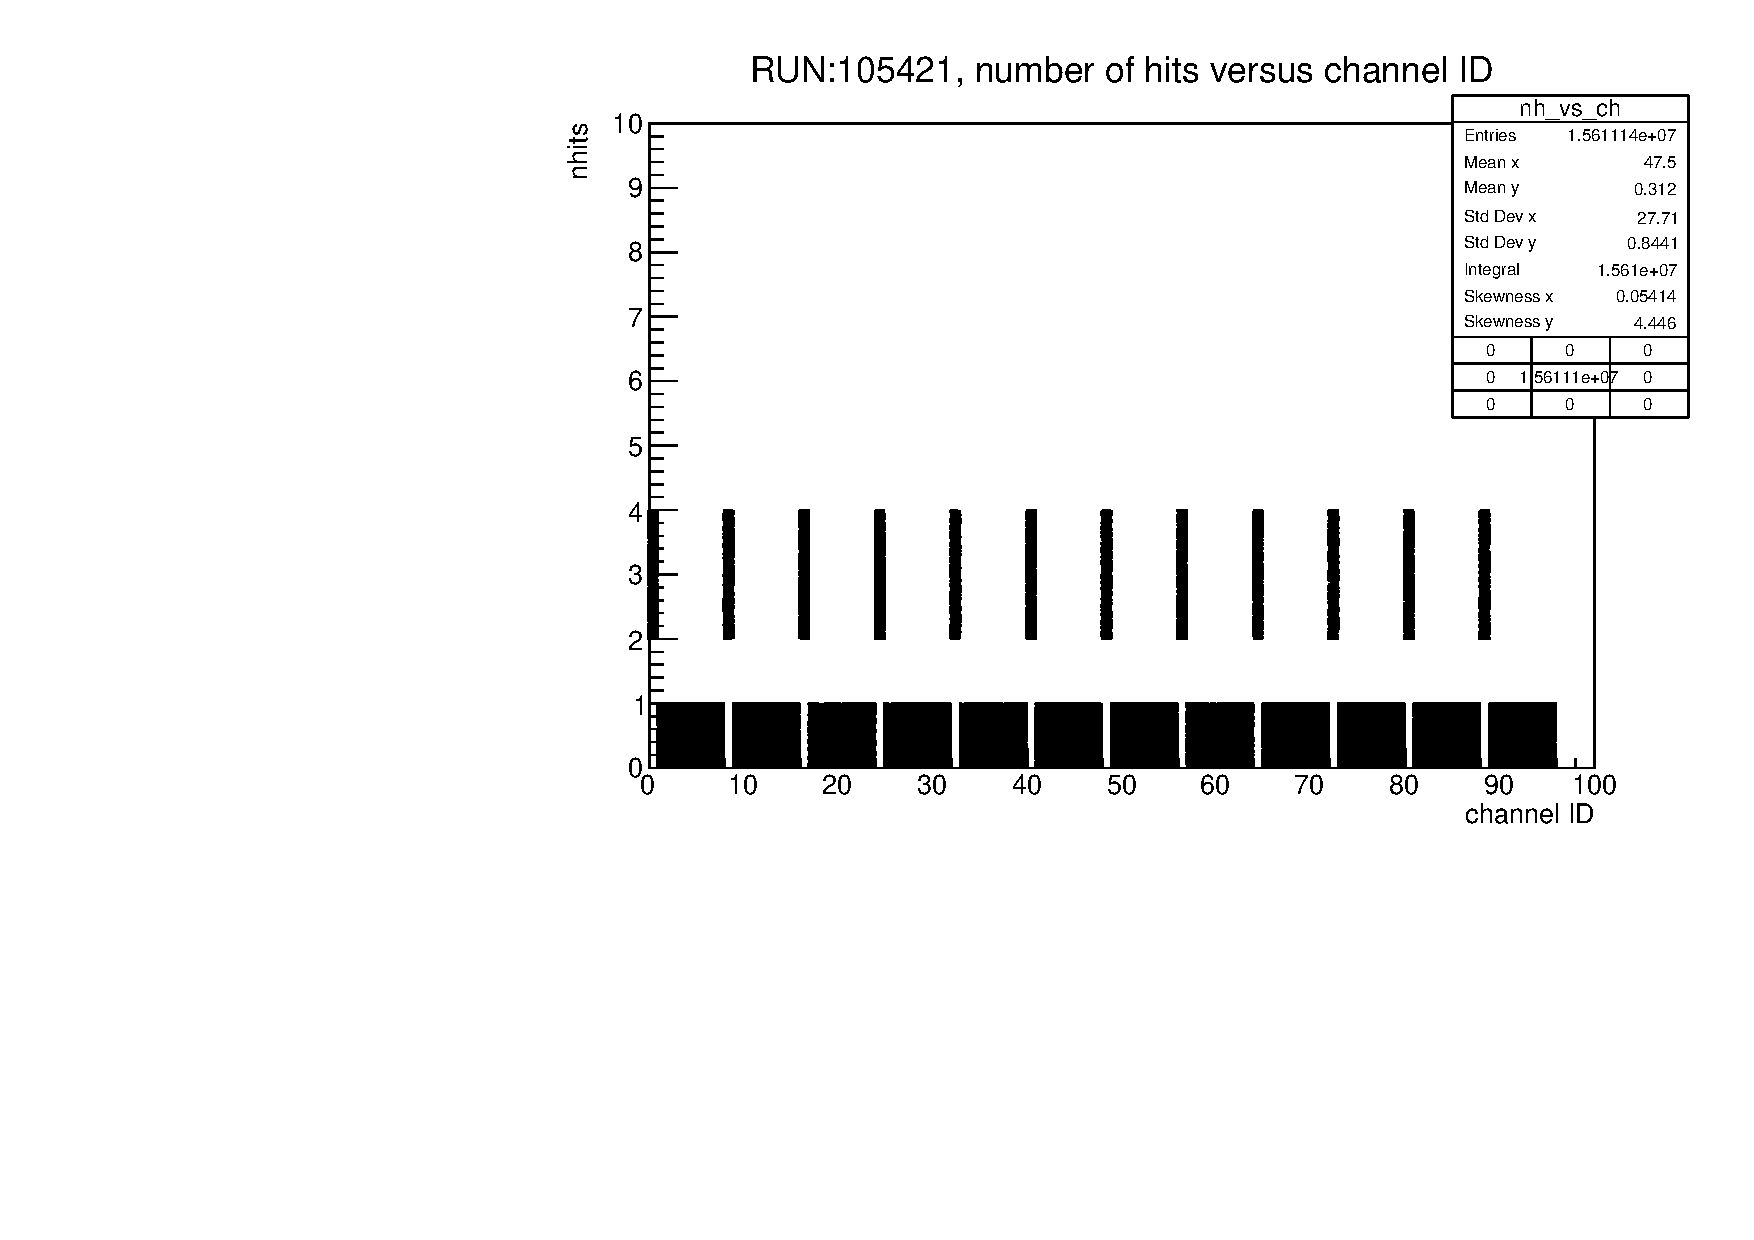
\includegraphics[width=0.65\textwidth]{figures/pdf/run105421_nh_vs_ch.pdf}
      \caption{Regular distribution of number of hits versus channel ID. 
      The 0th channel is the first to be pulsed.
      As a consequence, the active channels are the 8th, 16th, 24th, 
      32nd, 40th, 48th, 56th, 64th, 72nd, 80th and 88th. 
      The number of hits is 3 or 4 for all channels. 
      No cross talks were observed in any neighbour channel.}
     \label{fig:normalhits}
\end{figure}
Figure \ref{fig:dead} shows a run with one dead channel (ID=94) 
and a channel (ID=70) with more than three hits, which was not expected. 
In the case of the dead channel, the problematic preamp 
was replaced. In the second case, to investigate this more thoroughly, 
I made the distribution of the time difference 
$\Delta t$ distribution between consecutive pulses (Figure \ref{fig:deltatnhits}).
Since the pulser provides pulses at the frequency of 50 kHZ, the $\Delta t$ 
distribution should show one single peak at 20 $\mu$s. 
On the other hand, there are also two pronounced peaks at 16 $\mu$s and 4 $\mu$s. 
In particular, the analysis of the waveforms of the hits in the 4 $\mu$s peak 
showed an inversion of the waveforms: this has been further investigated 
and will be discusse in more detail in Section \ref{wf}.
\begin{figure}[!h]
  \centering
  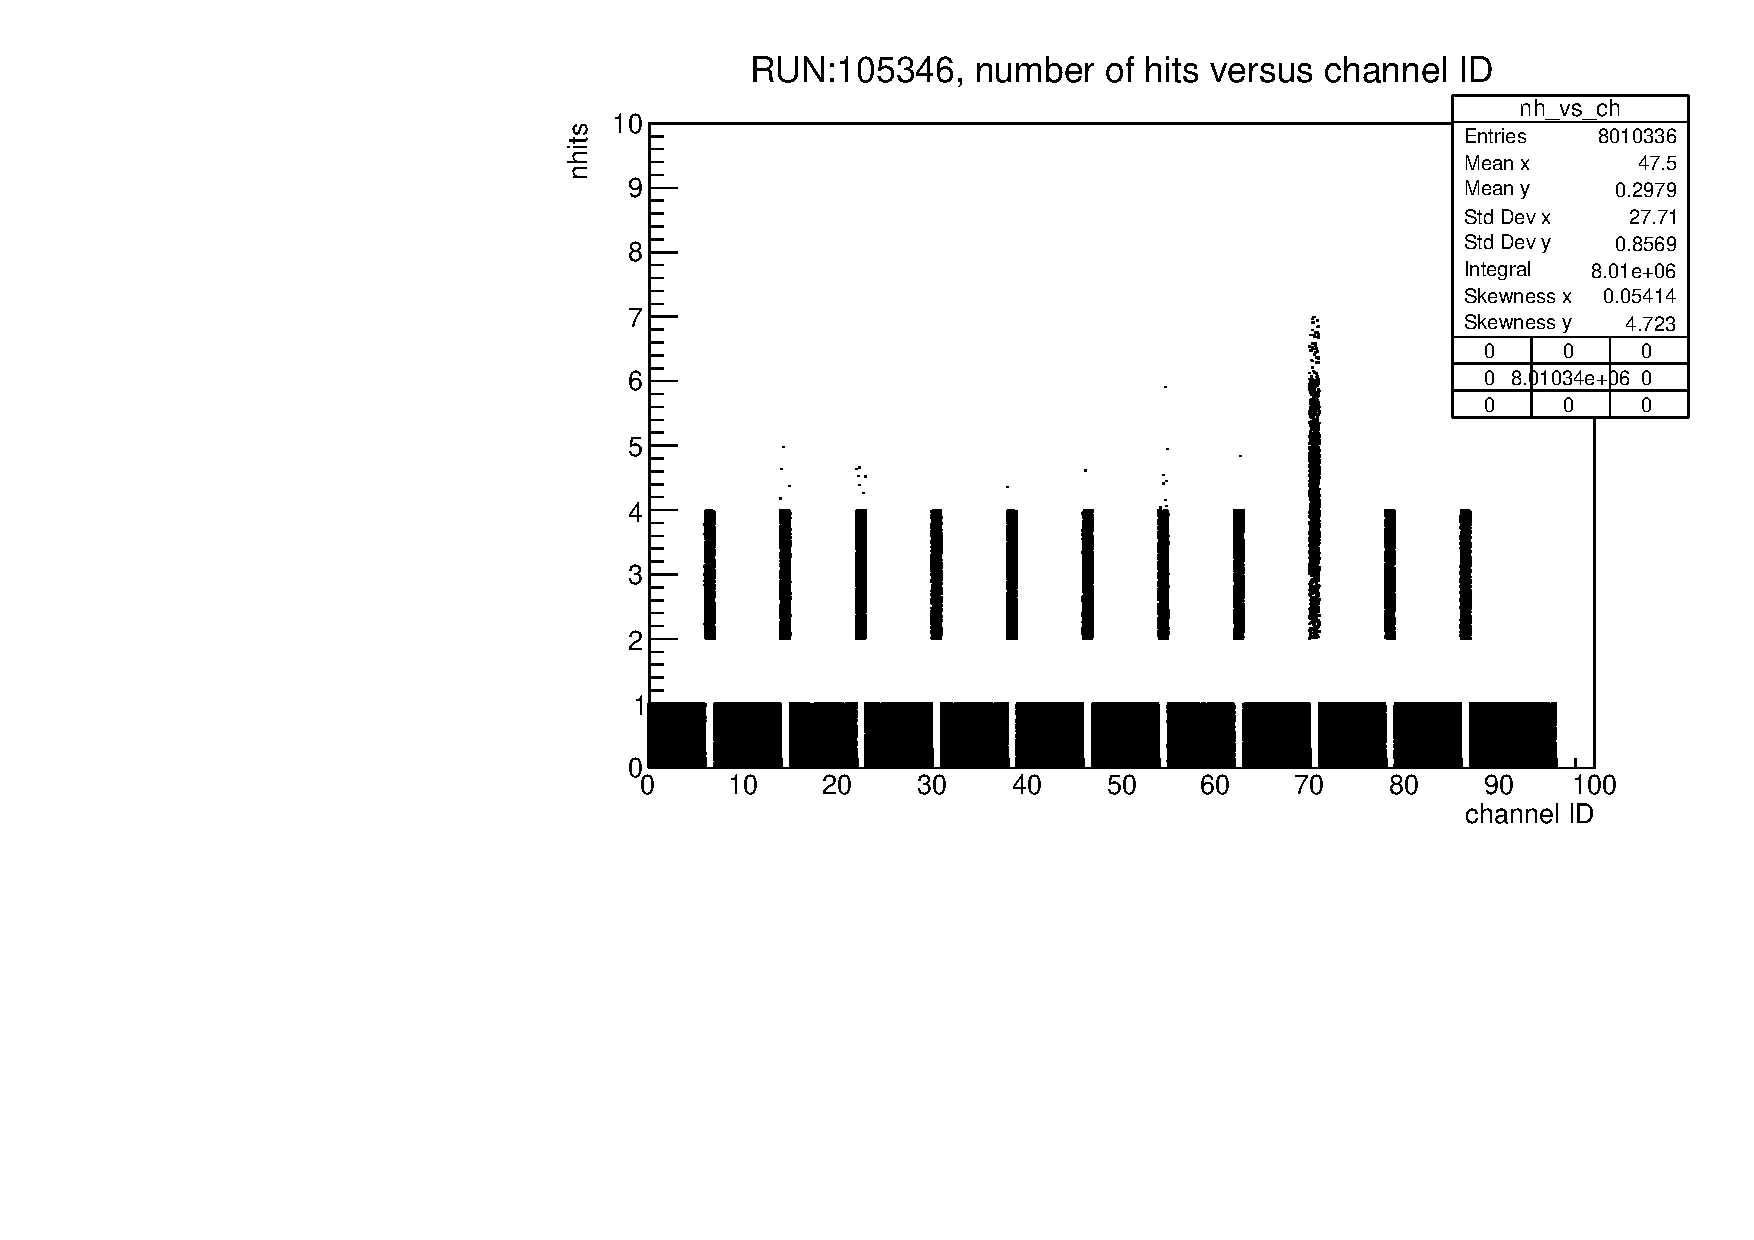
\includegraphics[width=0.65\textwidth]{figures/pdf/run105346_nh_vs_ch.pdf}
  \caption{Distribution of number of hits versus channel ID. 
  The 6th channel is the first to be pulsed.
  As a consequence, the channels that should be active are the 
  14th, 22nd, 30th, 38th, 46th, 54th, 62nd, 70th, 78th, 86th and 94th. 
  The 94th channel is not responding. In this case, the preamp 
  was substituted. The number of hits is not the same 
  for all channels. The 14th, 22nd, 38th, 46th, 54th, 62nd, 
  70th channels have more hit than expected.
  To address this issue, the distribution of $\Delta t$ between 
  hits of one of this channels is reported in Figure \ref{fig:deltatnhits}.
  No cross talks were observed in any neighbour channel.}
 \label{fig:dead}
\end{figure}


\begin{figure}[!h]
  \centering
  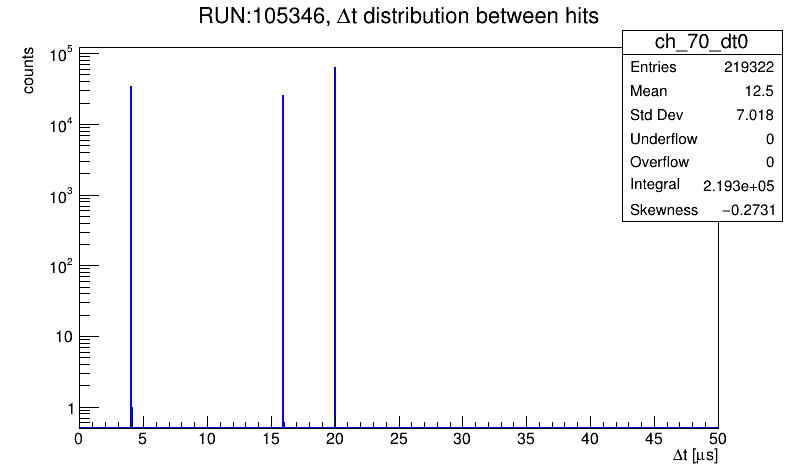
\includegraphics[width=0.65\textwidth]{figures/png/deltathits.png}
  \caption{$\Delta t$ distribution between hits in the 70th channel. The $\Delta t$ distribution between hits 
  should peak at 20 $\mu$s, as the pulser operates at a frequency of 50 kHz. However, peaks at approximately 
  16 $\mu$s and 4 $\mu$s are observed. All waveforms at around 4 $\mu$s are inverted compared to the regular ones. 
  The waveforms are shown in Section \ref{wf}, and the reason for this behaviour will be explained in the same section.}
 \label{fig:deltatnhits}
\end{figure}

Figure \ref{fig:cross} shows a clear example of cross-talk among channels. 
We tried to characterize this phenomenon and we noticed that it occurred 
only when the ID of the first channel to be pulsed is odd.
The cross talk was also asymmetric (3$\rightarrow$5 was observed, 
but no 3$\rightarrow$1).
As described in Chapter \ref{chaptertrk} and shown in Figure \ref{fig:spacepreamps}, 
the preamps are mounted on vertical boards and one preamp is 
connected to two straw-tubes: odd channels are the ones on the board, 
while even ones are on the top. For this reason, the cross talk 
appears to be between channels plced on the board. 
Moreover, we observed the cross-talk only in the first 20 channels IDs.
This is due to the fact that the distance between consecutive preamp 
boards is slightly narrower for the first channels (Figure \ref{fig:spacepreamps}).
\begin{figure}[!h]
  \centering
  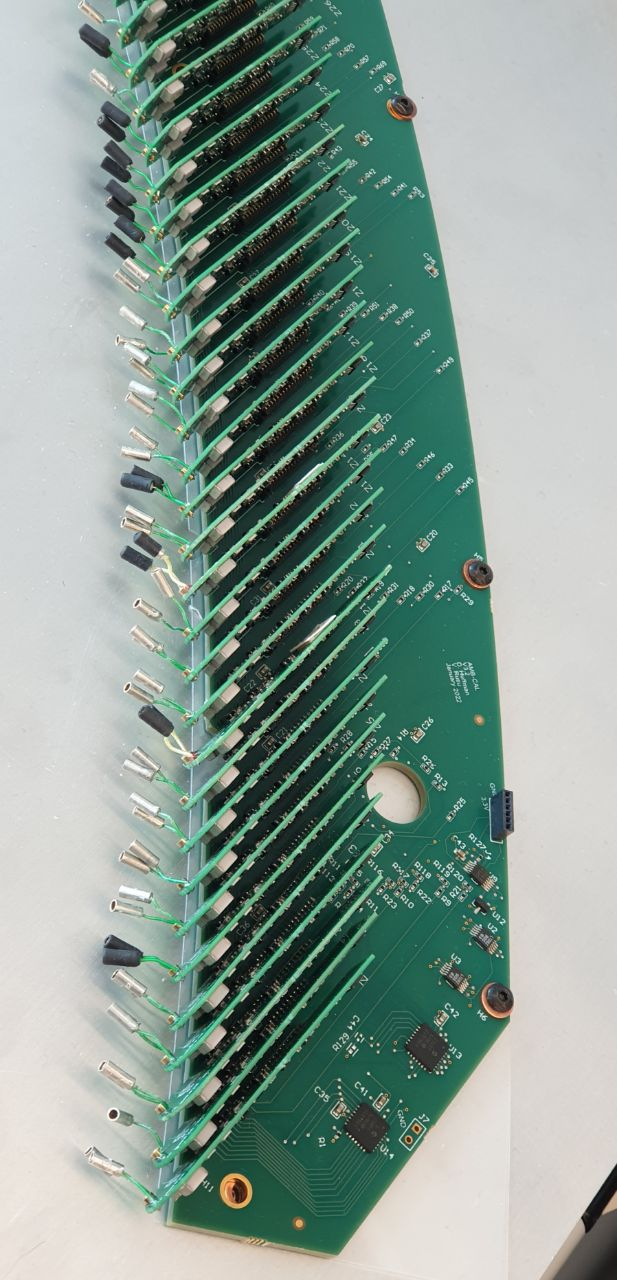
\includegraphics[angle=90,width=0.8\textwidth]{figures/jpg/photo_6028424923279639562_y.jpg}
  \caption{The spacing between preamps on the board. The first channels correspond to the preamps on the right side of the picture.}
 \label{fig:spacepreamps}
\end{figure}
The ouput of the test was reported to the tracker panel 
experts, and they are still working on it.
\begin{figure}[!h]
  \centering
  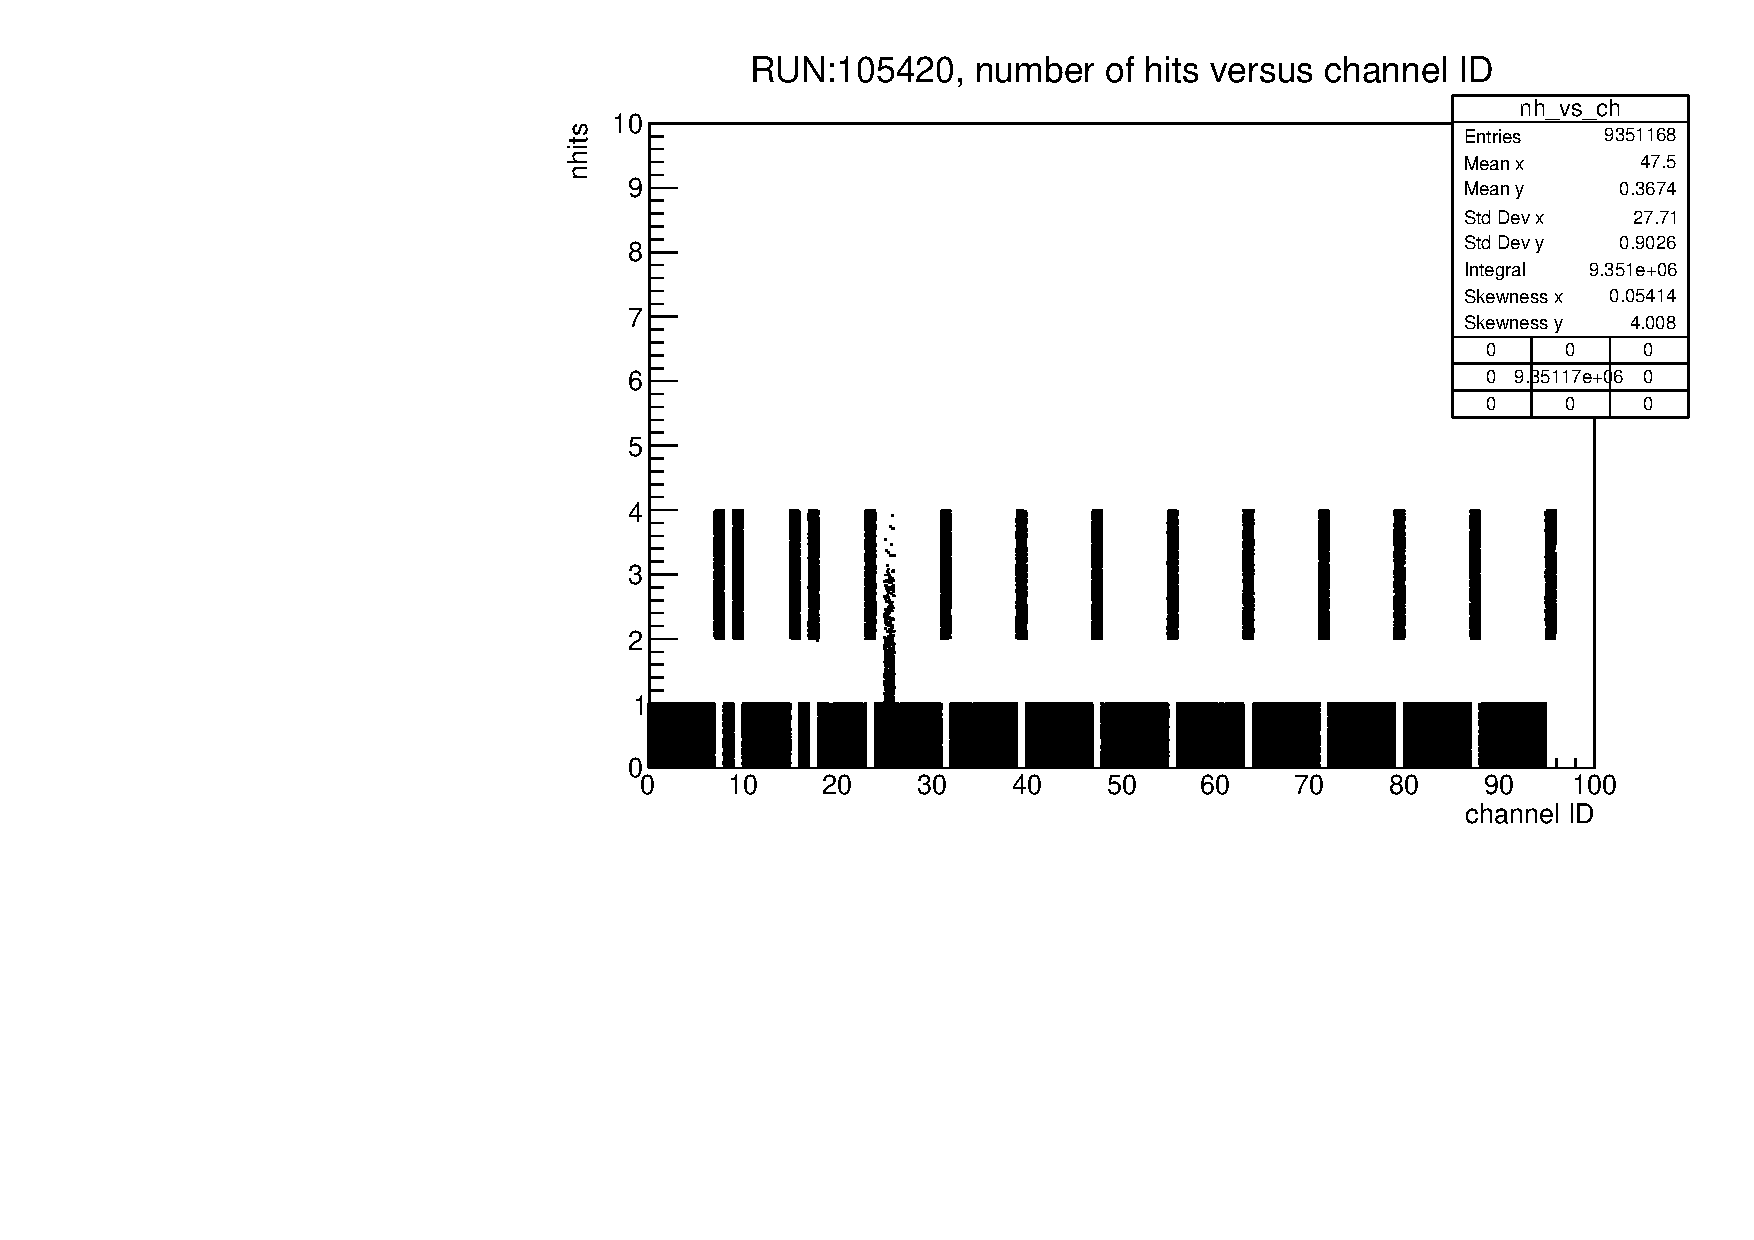
\includegraphics[width=0.65\textwidth]{figures/pdf/run105420_nh_vs_ch.pdf}
  \caption{Distribution of the number of hits versus channel ID. The 7th channel is the first to be pulsed. 
  As a consequence, the only channels that should be active are the 15th, 23rd, 31st, 39th, 47th, 55th, 63rd, 71st, 79th, 87th and 95th. 
  Channels 9th, 17th and 25th were also observed to be active, indicating cross talks.}
 \label{fig:cross}
\end{figure}
\subsection{Test 2: Analysis of the readout pulses waveforms}\label{wf}
The test described in this Section involved the study 
of the reconstructed waveforms from charge injection. 
The sampling frequency of the ADC is 40 MHz, which results 
in waveform bin width of 25 ns (Section. \ref{DRAC}). 
The maximum number of samples for one waveform is 30. 
To reconstruct the waveform, the baseline is already subtracted (Section \ref{basel}). 
Figure \ref{fig:normalwf} shows an example of reconstructed waveform for RUN105421. 
The negative tail is generated by a 
differentiating circuit that shapes the signal 
using a high-pass filter. This circuit was adopted 
because at high count rates two pulses can overlap: a 
new pulse can arrive before the previous one 
has returned to zero, thus leading to an overlap 
with the initial pulse's undershoot. This overlap 
may reduce the apparent amplitude of the subsequent 
pulse and generated the undesired broadening of peaks 
in the energy spectrum. 
The filter does not affect the rapid leading edge 
of the pulse because the time constant of the differentiator 
is not small compared to the rise time.

\begin{figure}[!h]
  \centering
  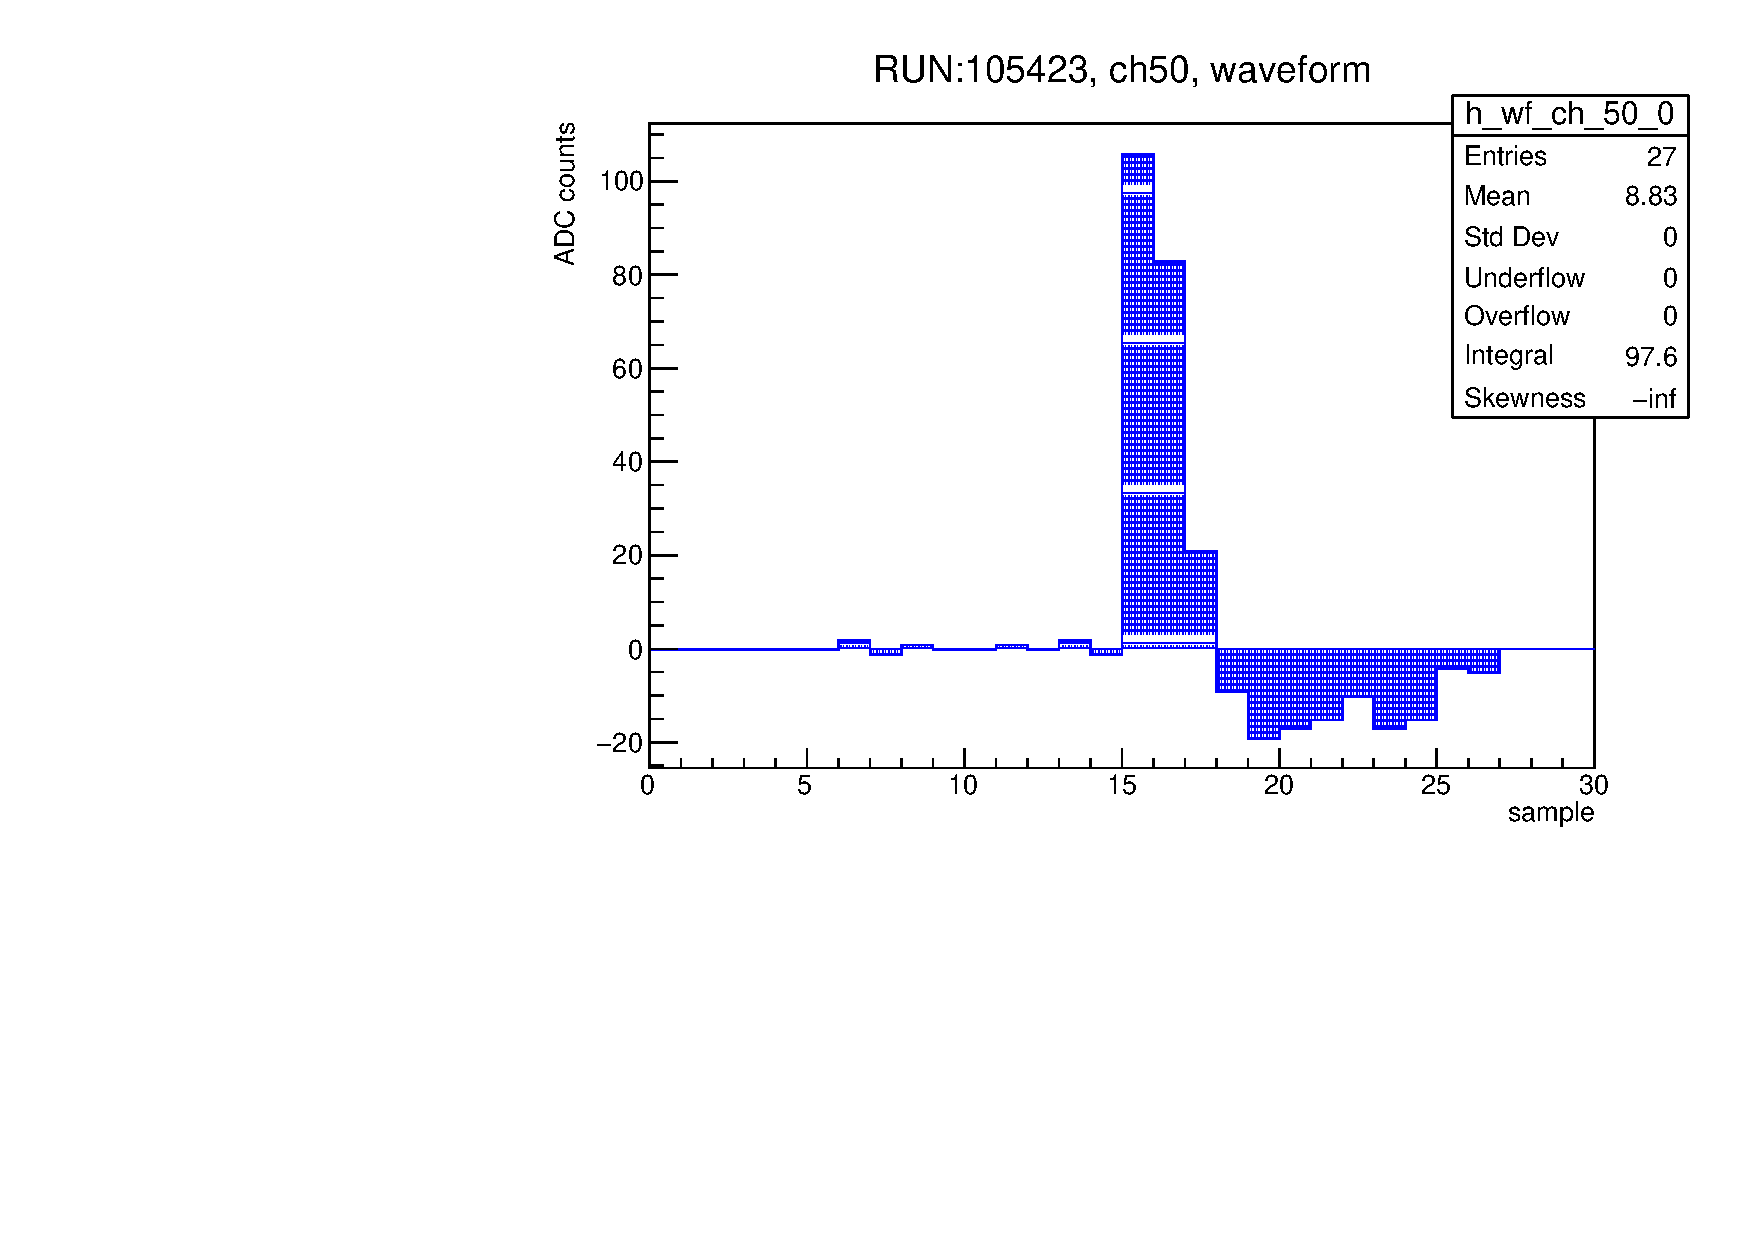
\includegraphics[width=0.65\textwidth]{figures/pdf/wf_ch50_0.pdf}
  \caption{Regular waveform of the 50th channel.}
 \label{fig:normalwf}
\end{figure}

As discussed in Section \ref{nhitvschid}, a larger number of hits than 4 
in channel 70 was observed, 
leading to a different $\Delta t$ distribution between hits than expected. 
While the $\Delta t$ peak was expected at 20 $\mu$s, in some channels two 
additional peaks were identified: 
one at 16 $\mu$s and another at 4 $\mu$s. The 4 $\mu$s peak is 
characterized by inverted waveforms (Figure \ref{fig:inverted}). 
The 16 $\mu$s peak is characterized by regular waveforms, as the 20 $\mu$s peak.
It is reasonable to think that this phenomenon arises from the erroneous 
generation of 4 $\mu$s long pulses, 
triggering them on both the leading and trailing edges. In fact, 
the sum of 4 $\mu$s and 16 $\mu$s is the inverse of the pulser frequency. 
One potential solution to address this issue could involve varying the pulse length. 
However, this approach was not pursued in this Thesis due to time constraints.
\begin{figure}[!h]
  \centering
  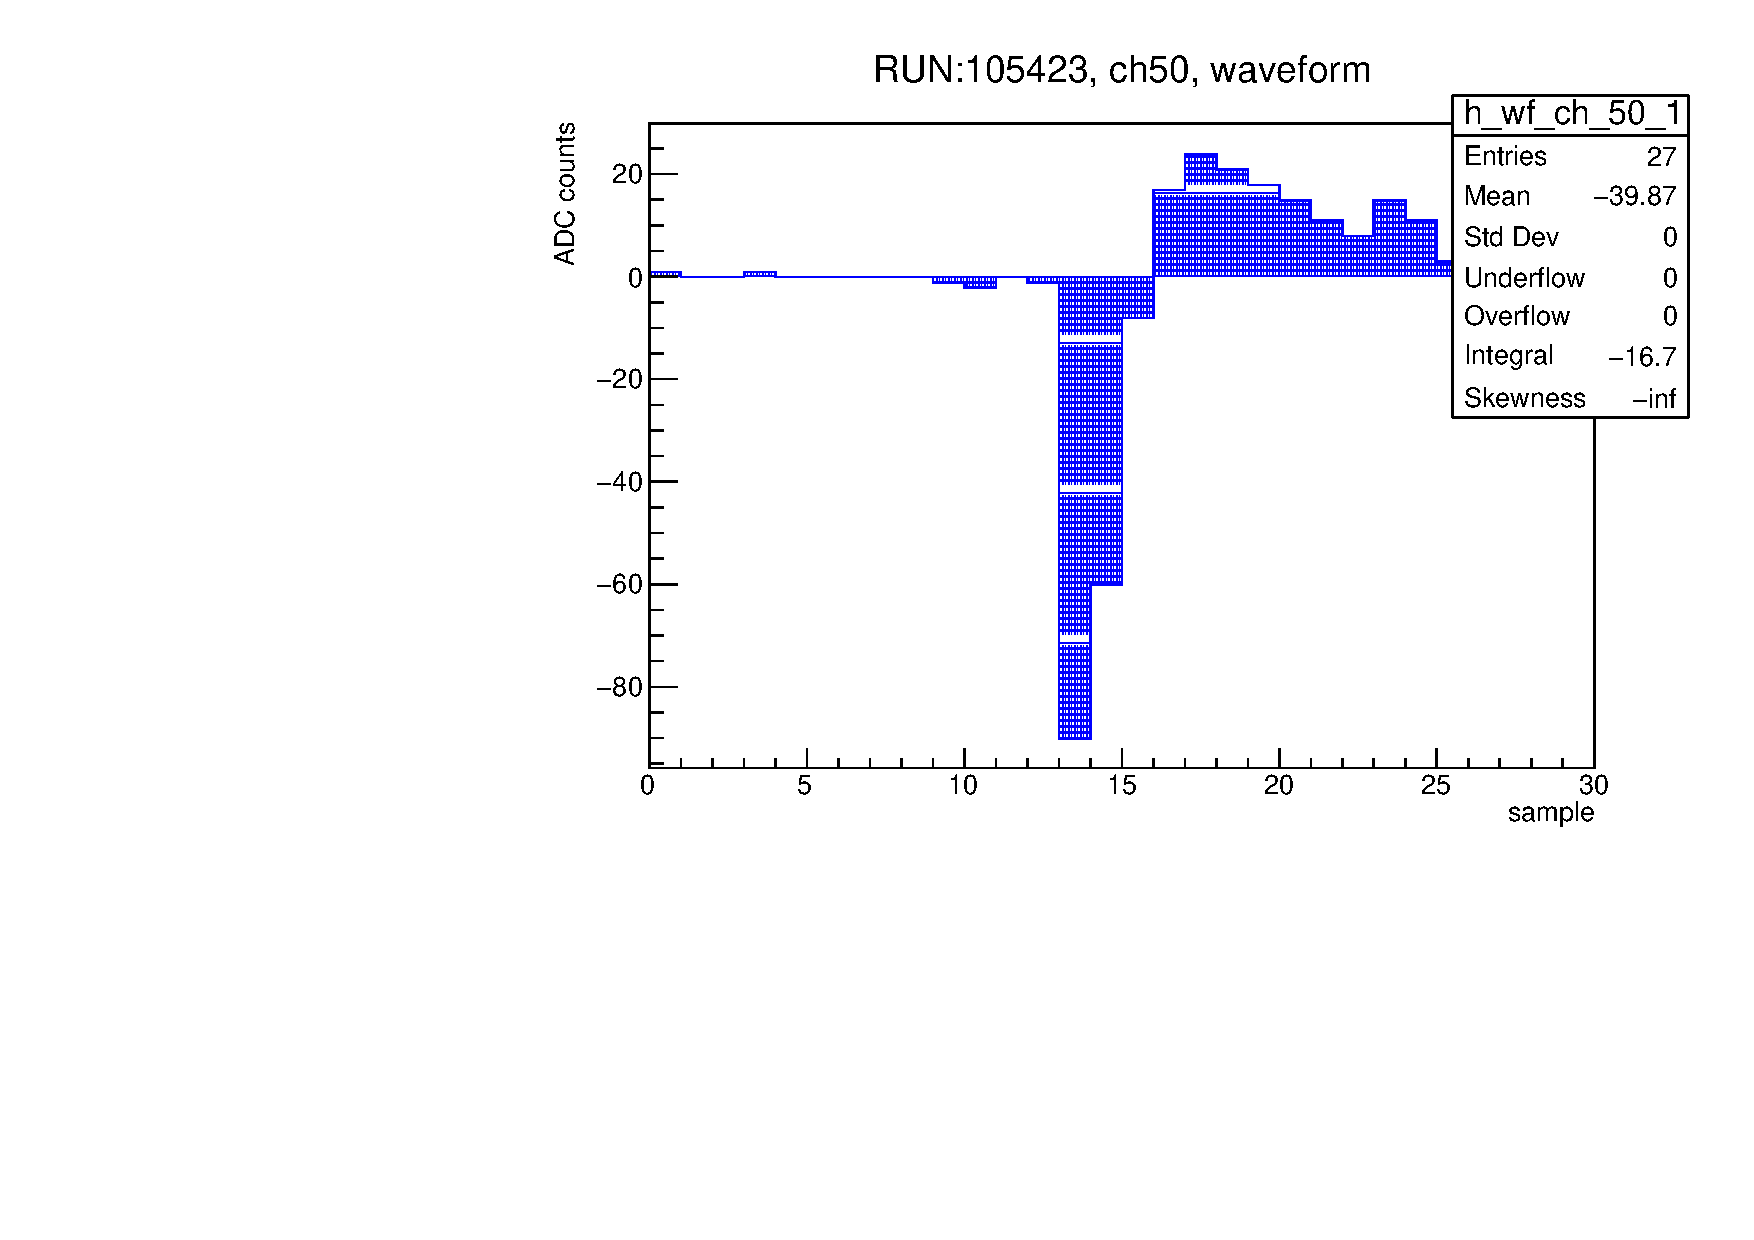
\includegraphics[width=0.65\textwidth]{figures/pdf/wf_ch50_1.pdf}
  \caption{Inverted waveform of the 50th channel.}
 \label{fig:inverted}
\end{figure}
\subsubsection{Estimating the waveform pedestal}\label{basel}
We adopted a straightforward procedure to estimate the pedestal: 
we simply take the mean value of the first 10 samples of the waveform. 
In each channel, the stability of the pedestal is an indicator of the 
level of noise within the electronic chain. 
The pedestals for each channel vary according on the electrical component's 
tolerances on the board.
Figures \ref{fig:baseline1} and \ref{fig:baseline2} show the distributions on 
the pedestals for two different channels, in a run named RUN105421.
In both cases, the pedestal is close to 210 ADC counts, with a 
FWHM$=2 \sqrt{2 \text{ln}2}\sigma\sim$4.5 ADC counts ($\sigma \sim$1.9 ADC counts).
  \begin{figure}[!h]
      \centering
      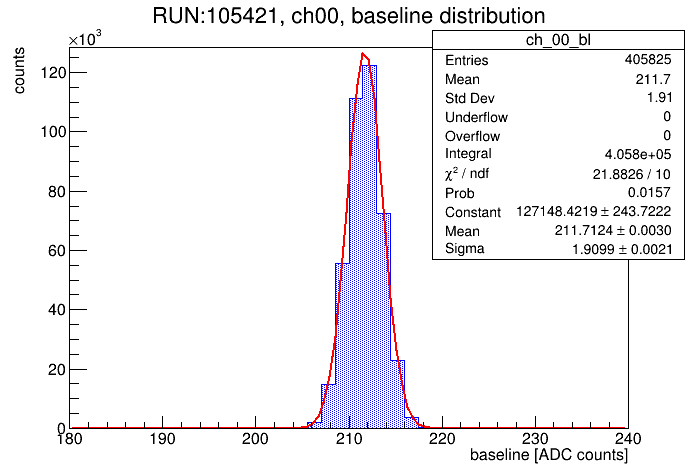
\includegraphics[width=0.65\textwidth]{figures/png/baseline_ch00.png}
      \caption{The fitted baseline distribution of channel 0.}
      \label{fig:baseline1}
  \end{figure}
  \begin{figure}[!h]
      \centering
      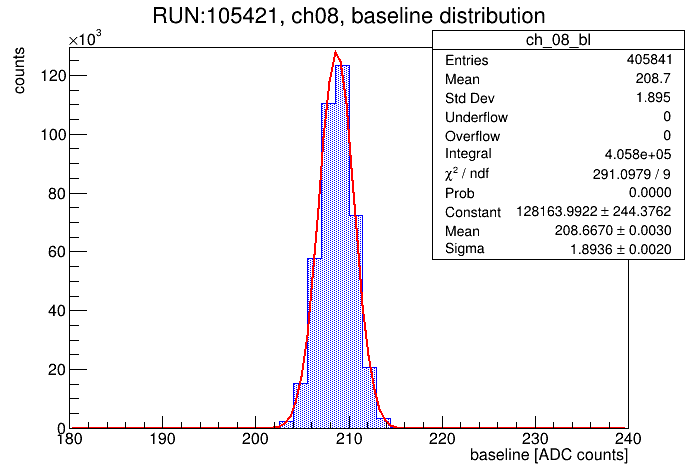
\includegraphics[width=0.65\textwidth]{figures/png/baseline_ch08.png}
      \caption{The fitted baseline distribution of channel 8.}
      \label{fig:baseline2}
\end{figure}

In some cases, a lower baseline value is observed. We observed dips of specific depths, 
for example 64, 128, or 192, which may suggest the possibility of malfunctioning 6th 
and 7th bit of the ADC (Figure \ref{fig:dips}). 
To address this issue, we simply disregarded the bins with the 
negative peaks and estimated the pedestals with the remaning samples.
\begin{figure}[!h]
  \centering
  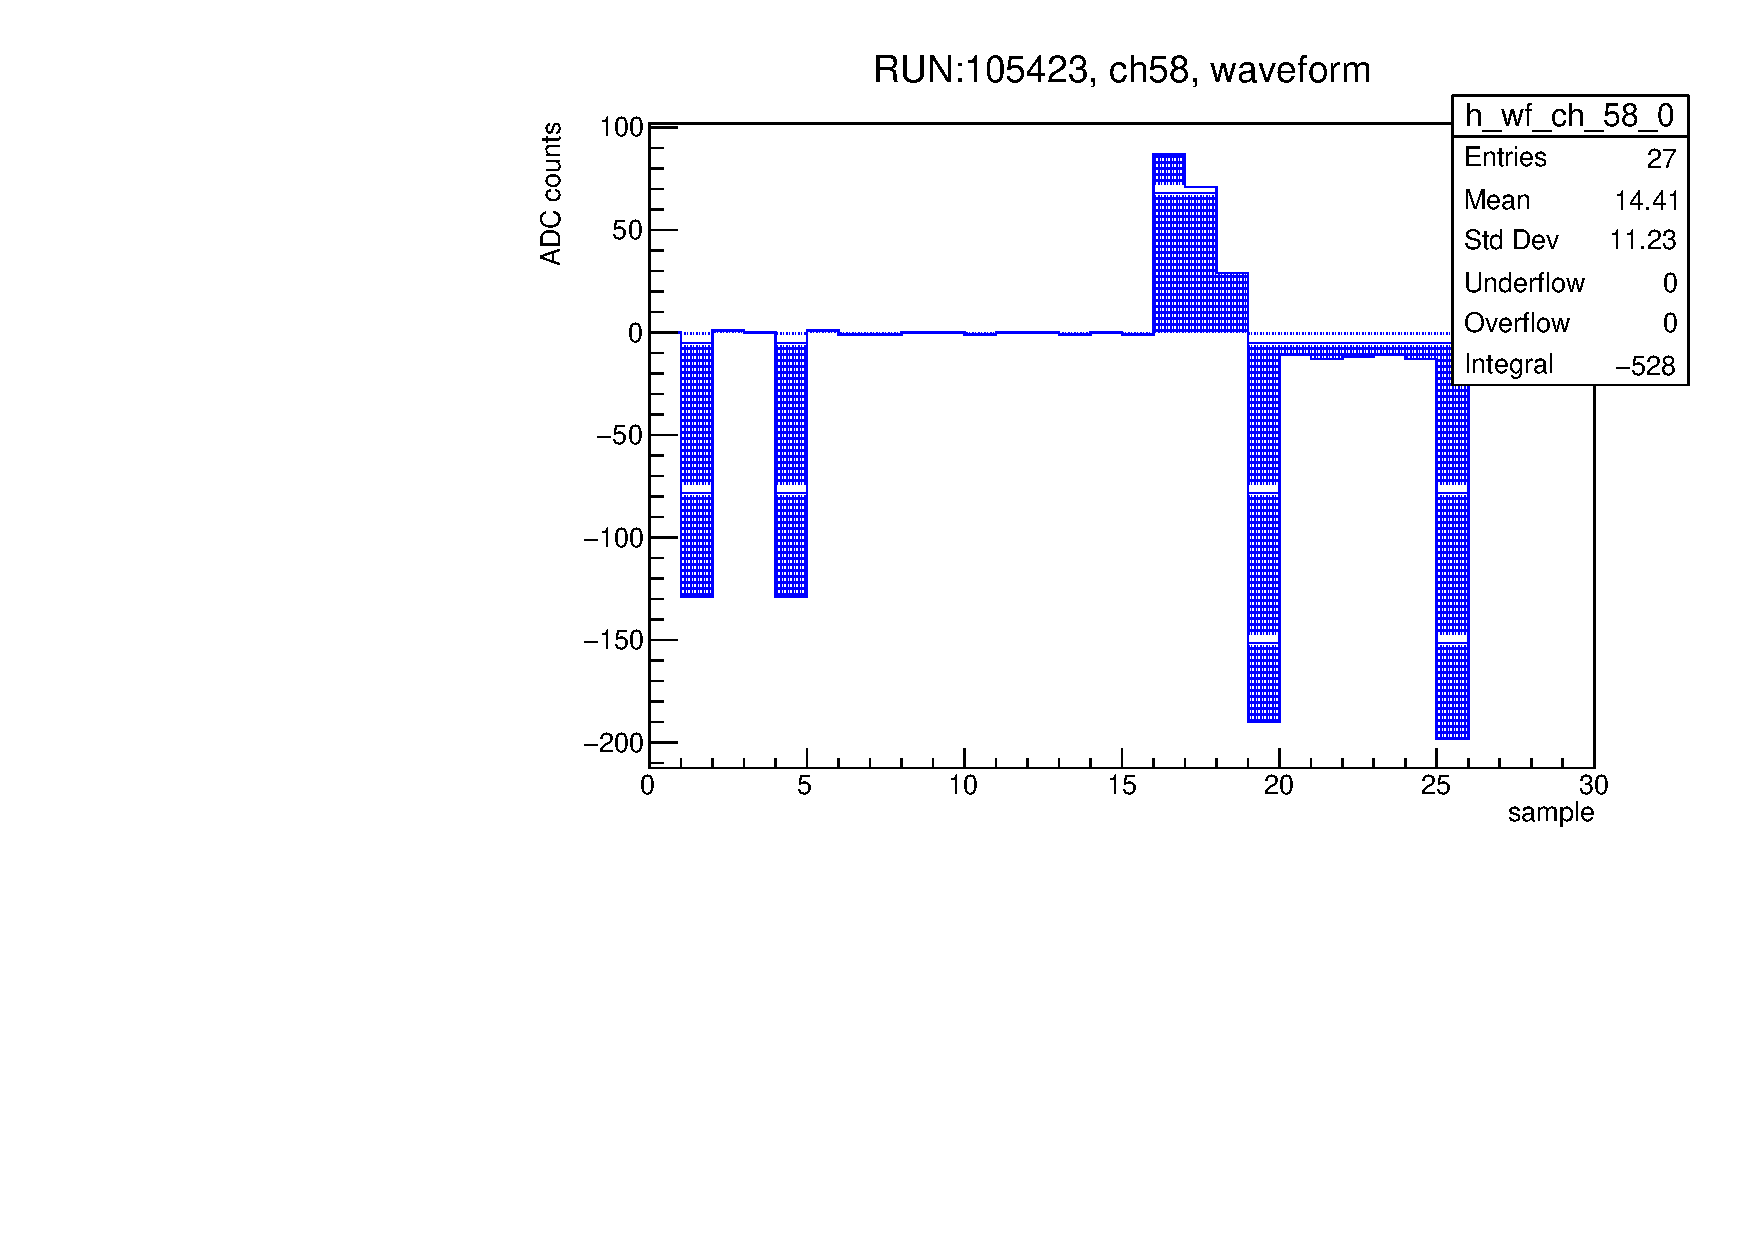
\includegraphics[width=0.65\textwidth]{figures/pdf/wf_ch58_1.pdf}
  \caption{Waveform of the 58th channel. Before subtracting 
  the baseline from the ADC counts, the dips were identified. The depth of the dips is 128.}
 \label{fig:dips}
\end{figure}
\subsubsection{The waveform charge and pulse height}\label{threshold}
Using a constant threshold discriminator, the integral of the positive and 
negative parts of the waveform, 
the pulse height and the first sample were computed. The threshold was set 
to 5 ADC counts. 
The first sample is defined as the first one to be above the threshold, 
and the positive charge 
is the integral of the region above the threshold. The negative charge 
is the integral of the waveform's 
negative tail. The pulse height is the highest ADC count reached 
by the waveform. The distributions of 
charge, pulse height, first sample and negative charge 
are shown in Figures \ref{fig:ch1}, \ref{fig:ph2}, \ref{fig:fs2}, and \ref{fig:nch2}.

\begin{figure}[!h]
      \centering
      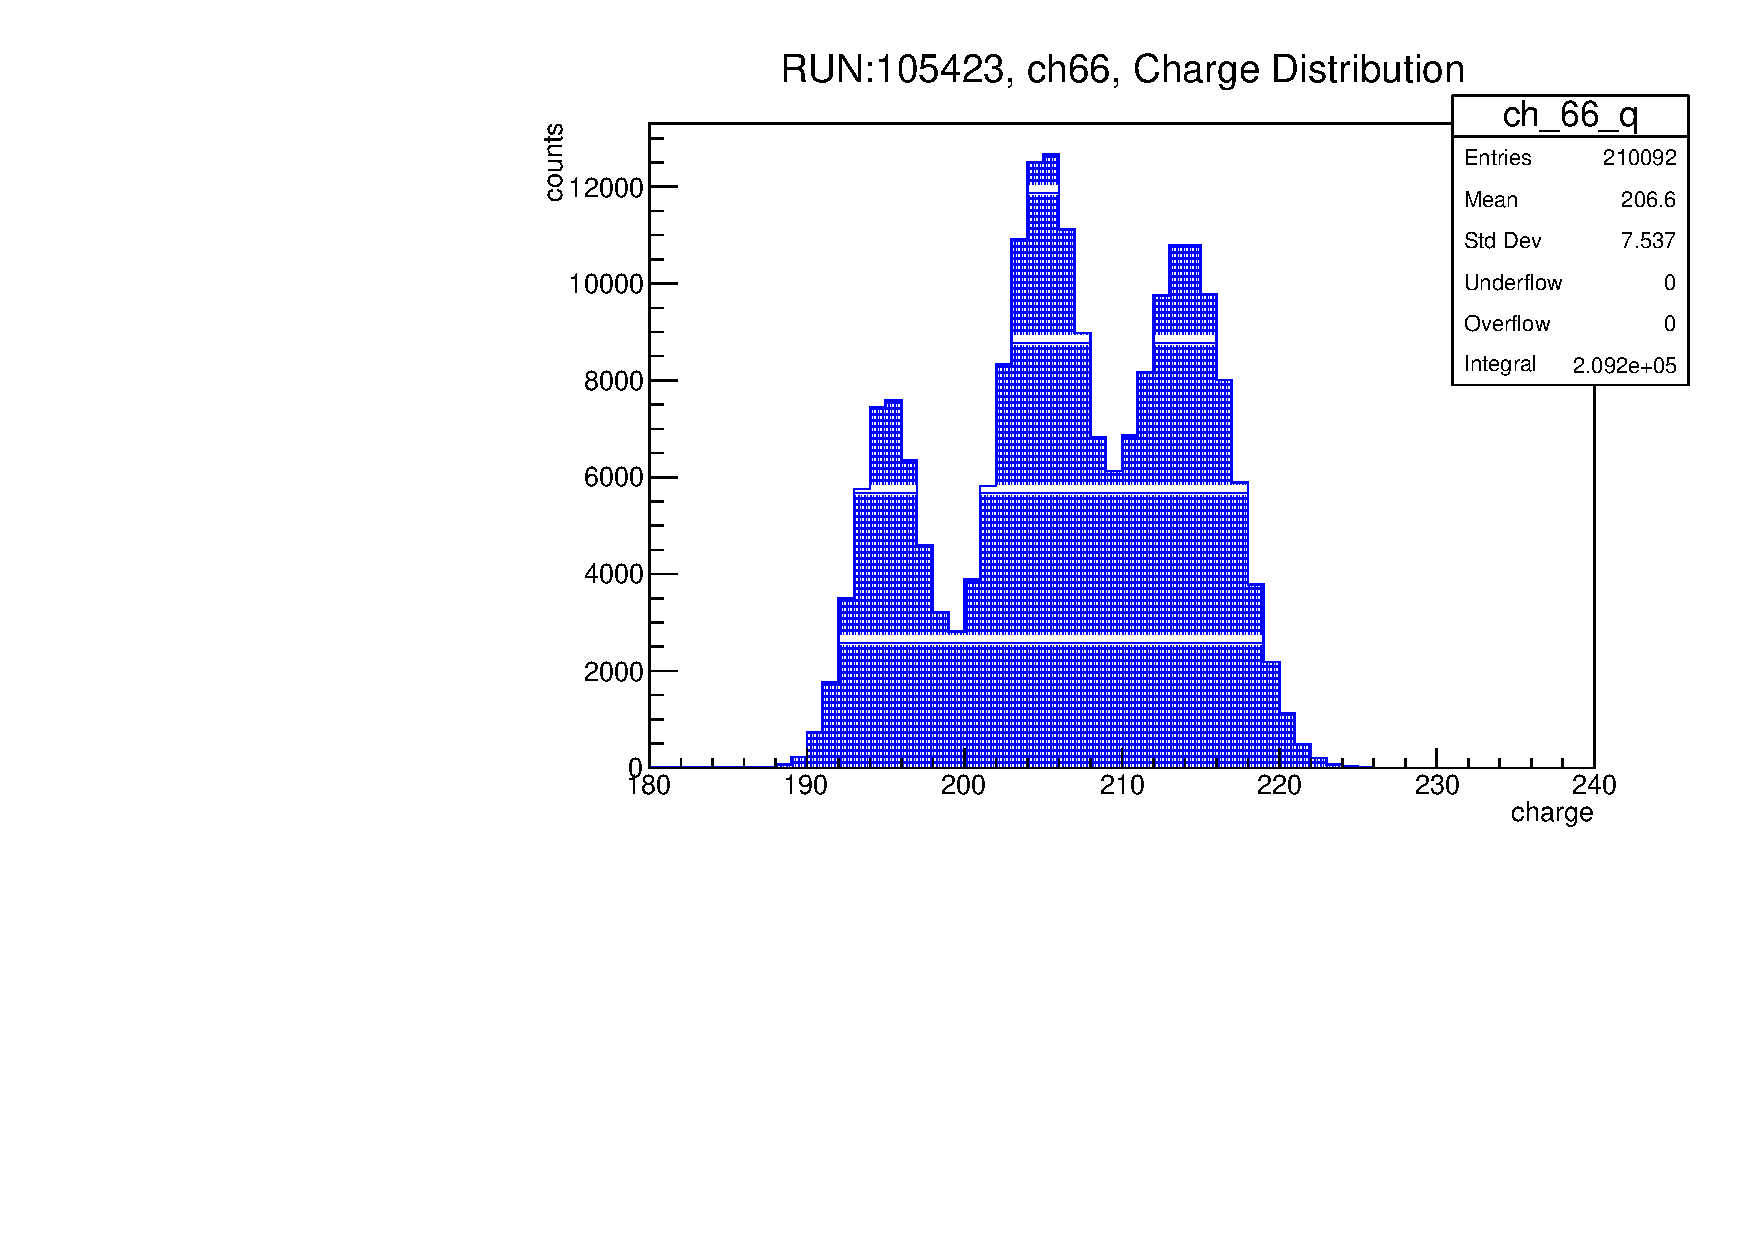
\includegraphics[width=0.65\textwidth]{figures/pdf/charge.pdf}
      \caption{Charge distribution of the waveforms in channel 66.}
      \label{fig:ch1}
  \end{figure}

\begin{figure}[!h]
  \centering
  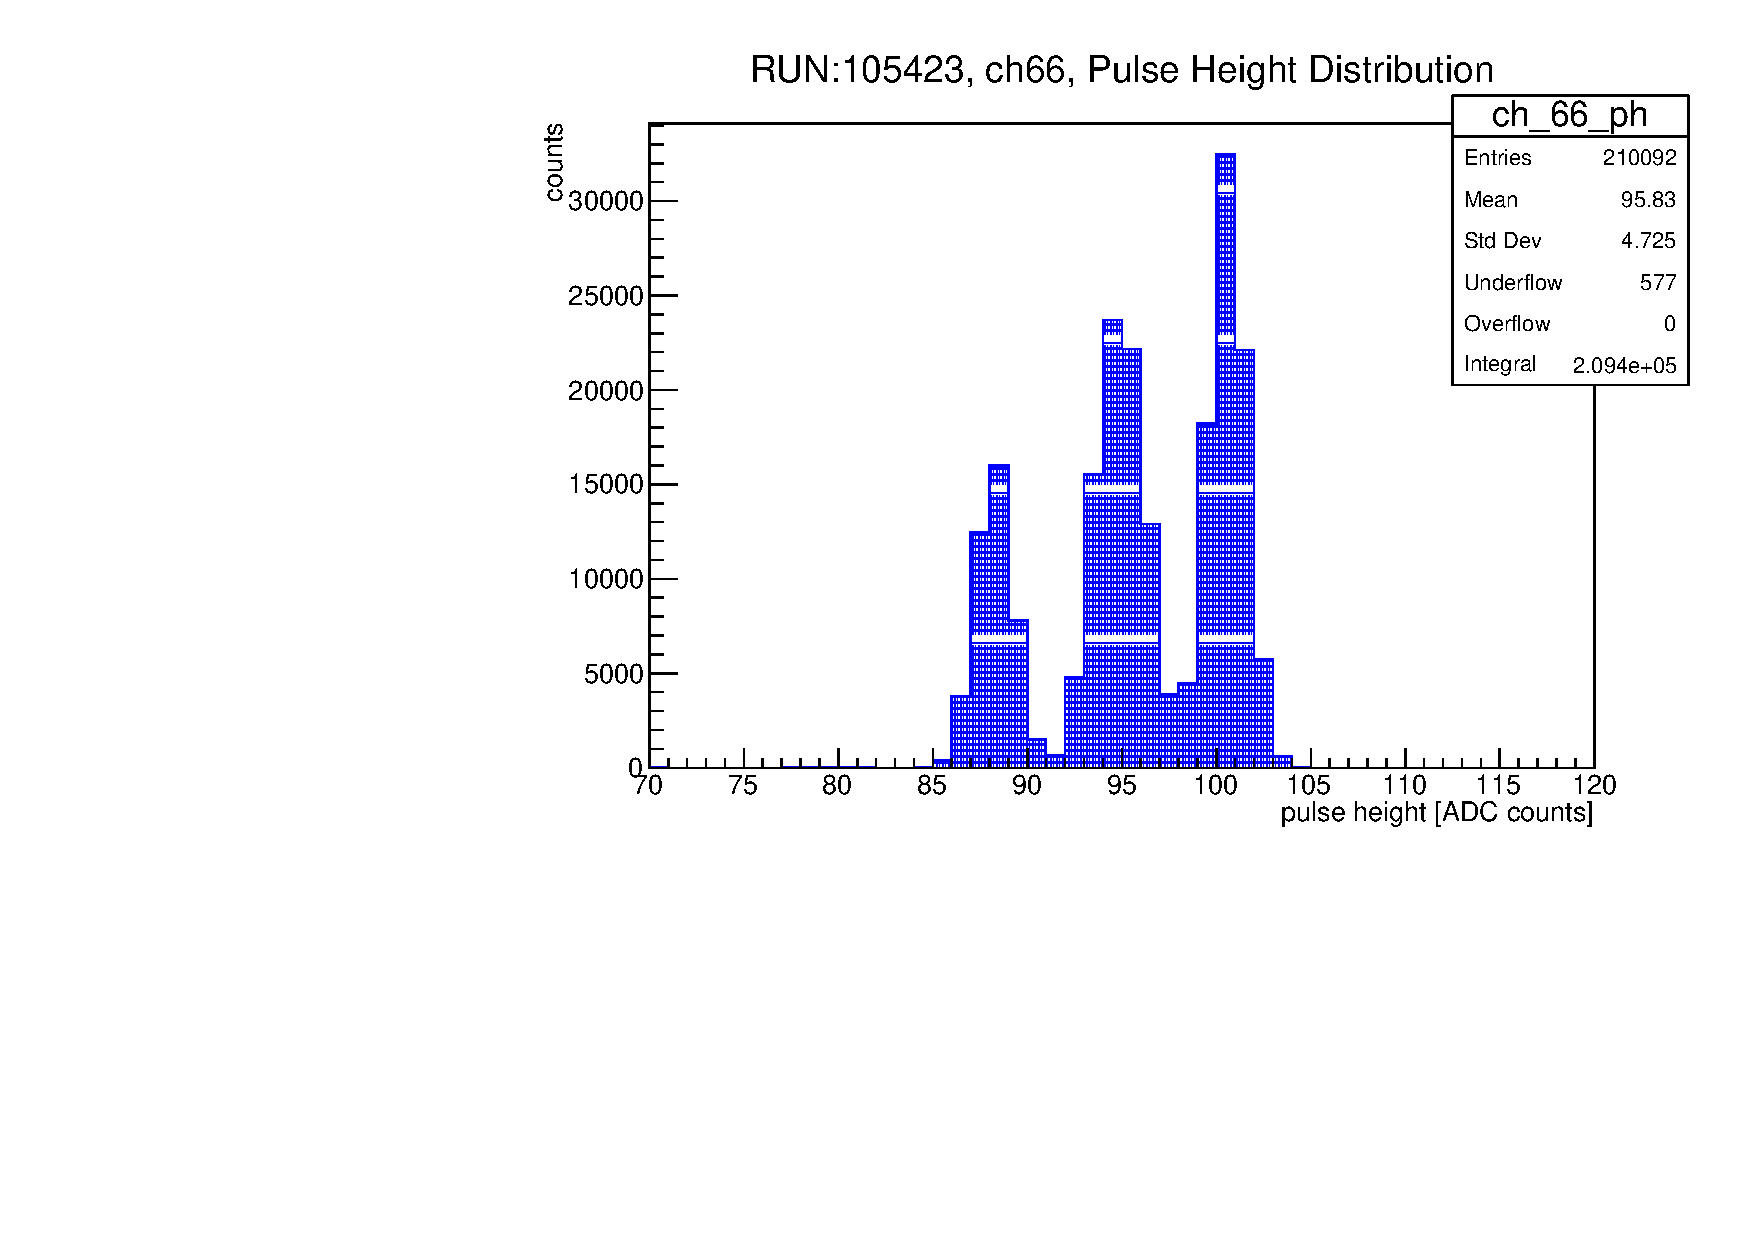
\includegraphics[width=0.65\textwidth]{figures/pdf/pulseheight.pdf}
  \caption{Pulse height distribution of the waveforms in channel 66.}
  \label{fig:ph2}
\end{figure}

\begin{figure}[!h]
  \centering
  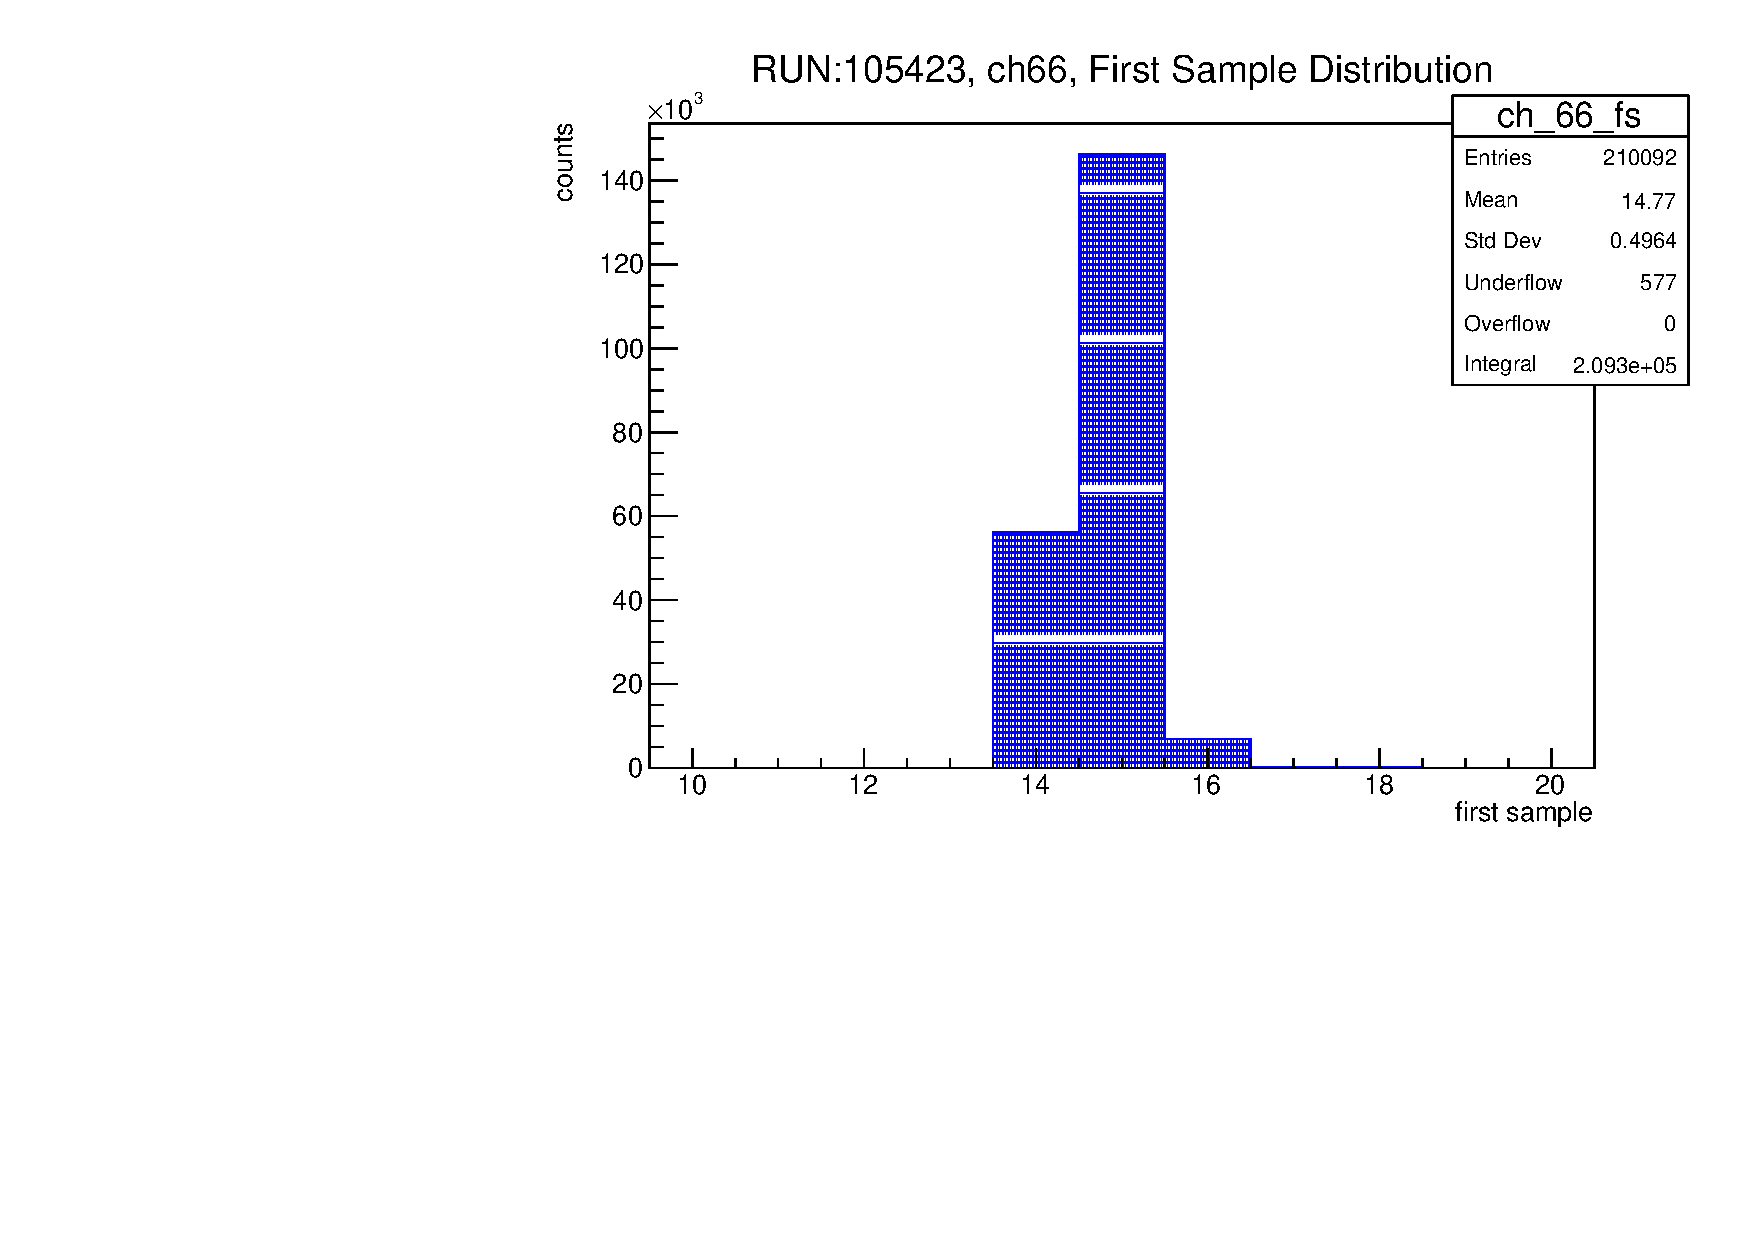
\includegraphics[width=0.65\textwidth]{figures/pdf/fs.pdf}
  \caption{First sample distribution of the waveforms in channel 66.}
  \label{fig:fs2}
\end{figure}

\begin{figure}[!h]
    \centering
    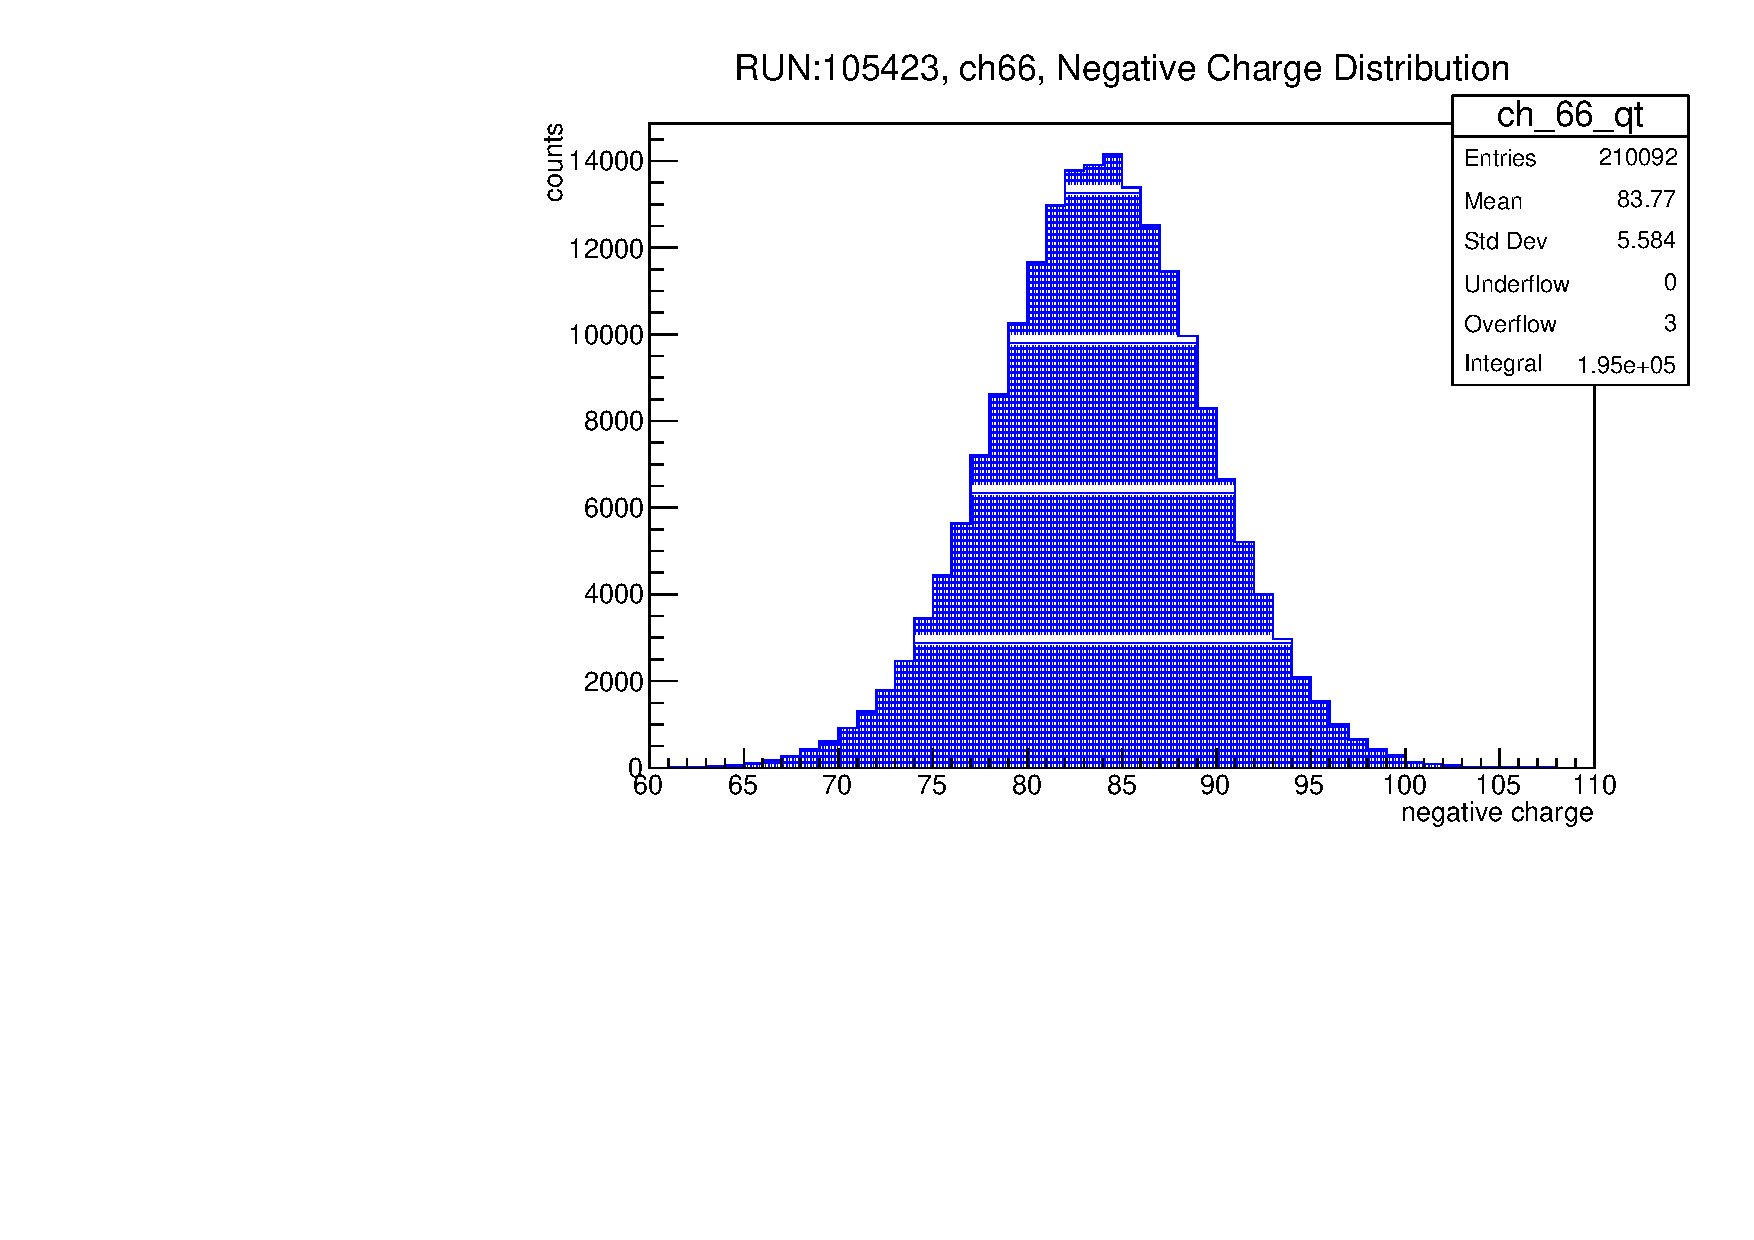
\includegraphics[width=0.65\textwidth]{figures/pdf/negcharge.pdf}
    \caption{Negative charge distribution of the waveforms in channel 66.}
    \label{fig:nch2}
\end{figure}
    
The charge and pulse height distribution exhibit a non-trivial shape. 
Three and two peaks were observed respectively; it was verified that 
these peaks were not correlated with the number of hits. Moreover, a 
correlation between the charge and pulse height peaks was observed, as shown in Figure \ref{fig:chvsph}. 
\begin{figure}[!h]
  \centering
  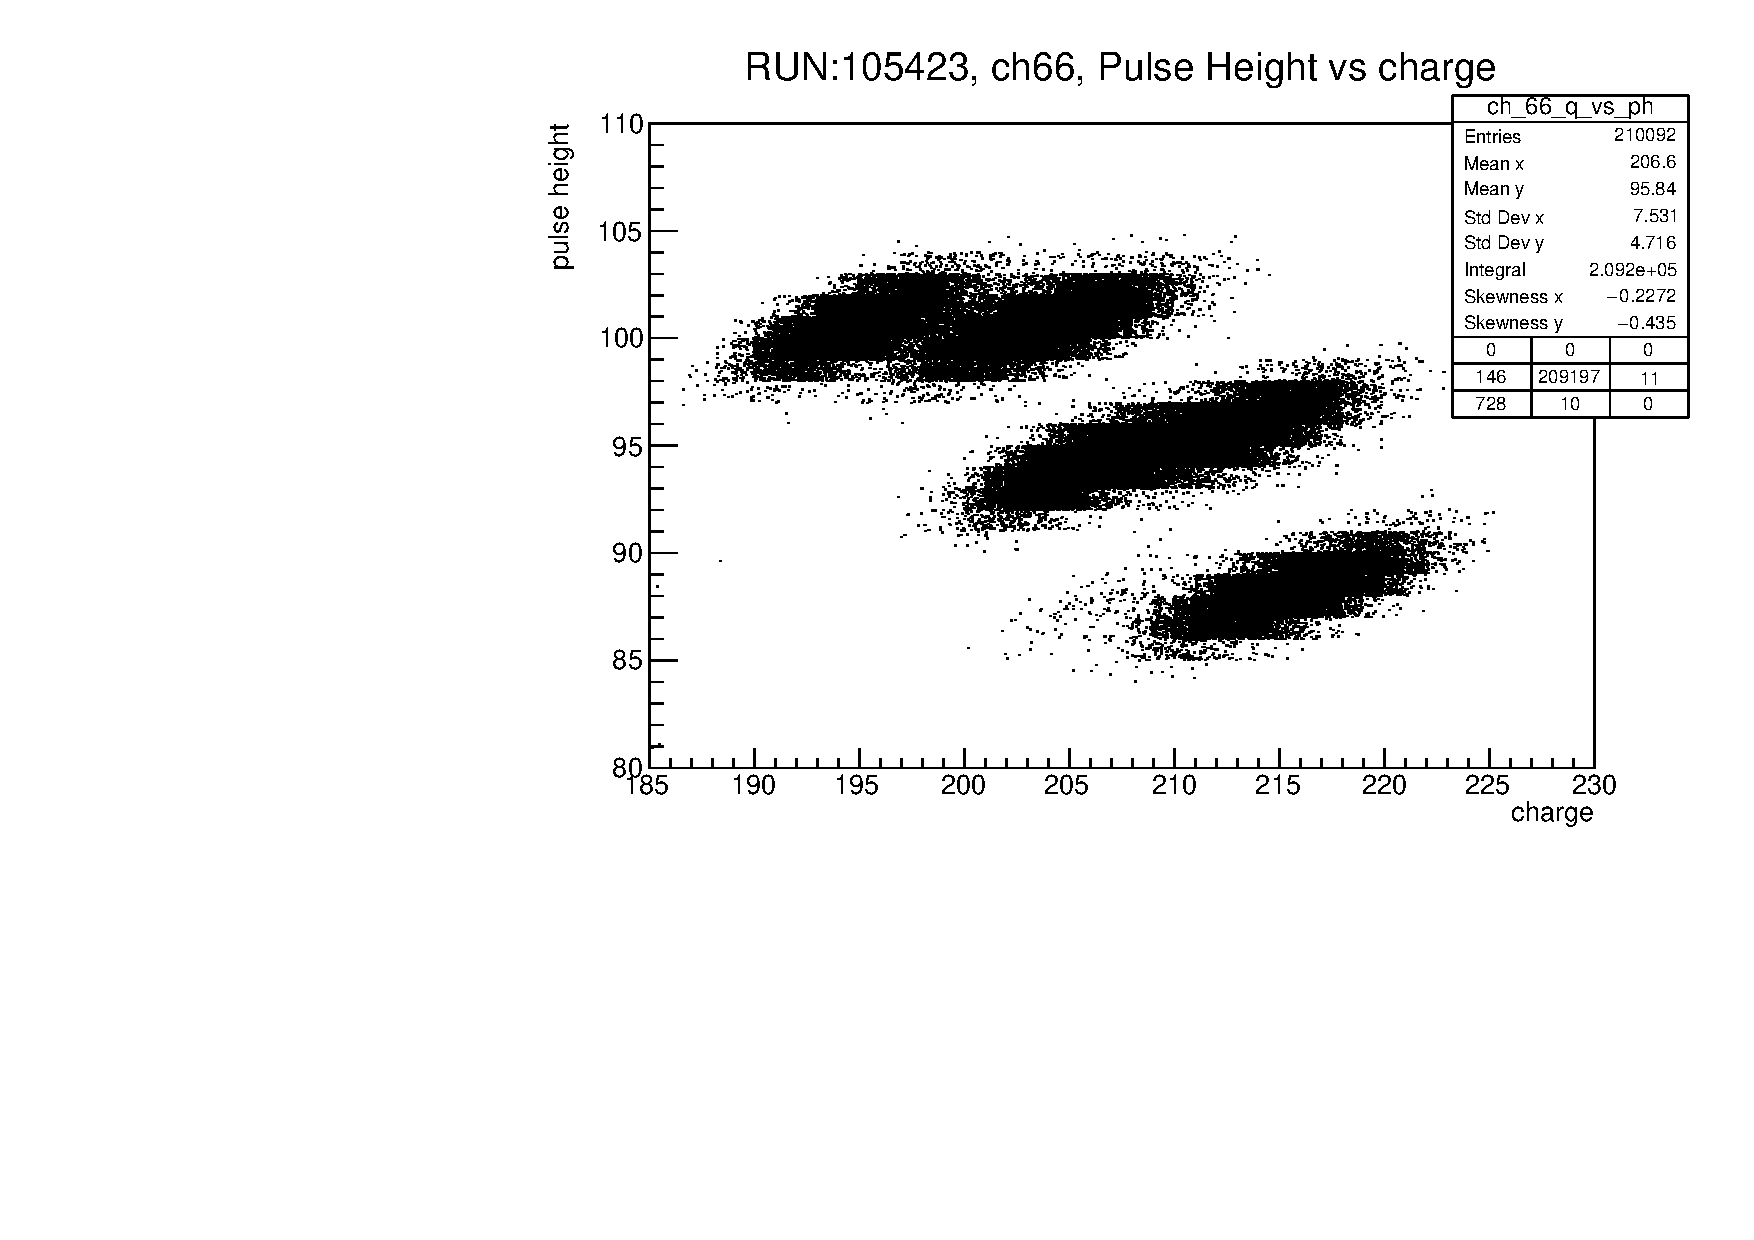
\includegraphics[width=0.65\textwidth]{figures/pdf/phch1.pdf}
  \caption{2D histogram of charge ($x$-axis) versus pulse height ($y$-axis).}
  \label{fig:chvsph}
\end{figure}
To understand the origin of this pattern, the waveform mean sample weighted with the charge 
\begin{equation} 
  s_{mean} = \frac{\sum_i \text{sample}_i \cdot q_i }{\sum_i q_i} 
\end{equation}
distribution was plotted in Figure \ref{fig:smean}. 
This plot shows that the time difference $\Delta s$ (approximately 2 ns) between pulses is less than the bin width, which is 25 ns. 
The next step was to check if $s_{mean}$ could be correlated with charge and pulse height peaks, 
as shown in Figure \ref{fig:chtm} and Figure \ref{fig:phtm}.
\begin{figure}[!h]
  \centering
  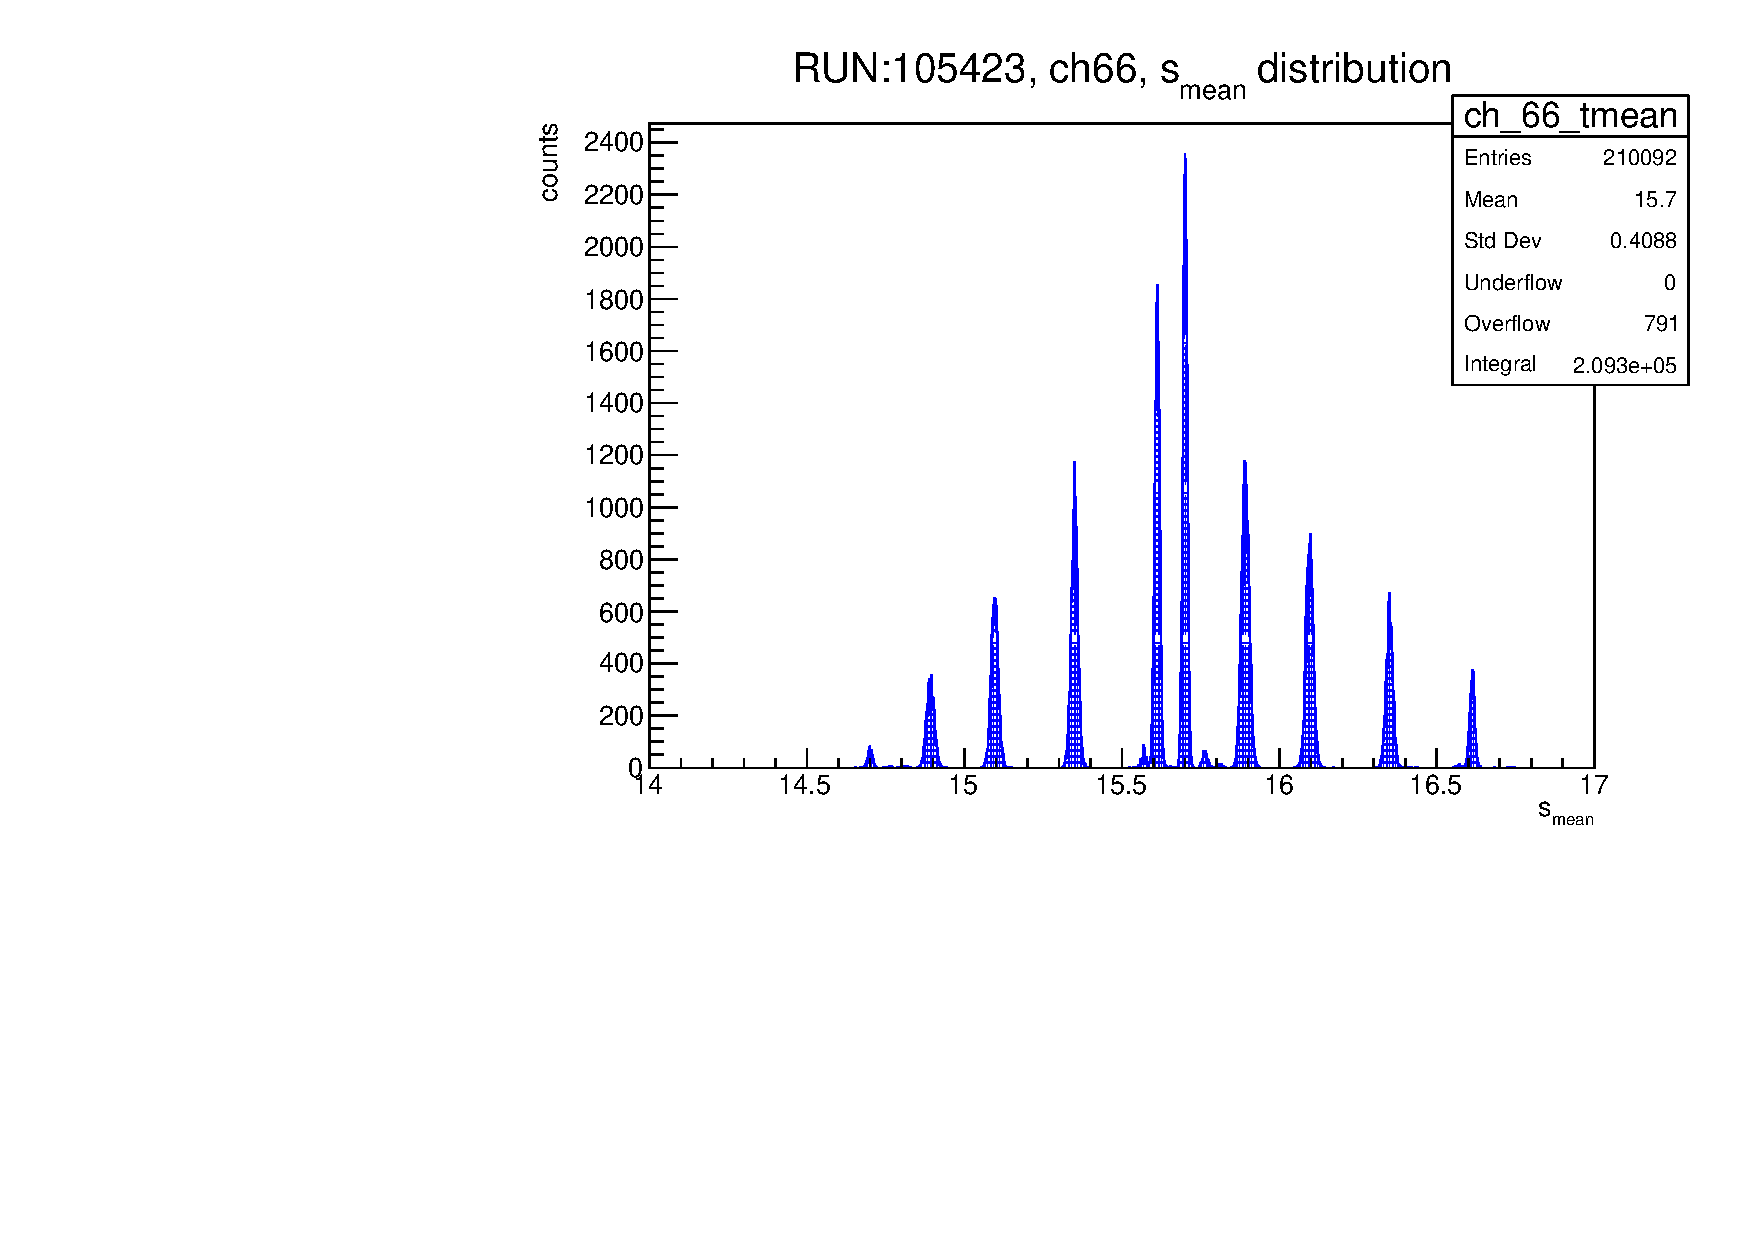
\includegraphics[width=0.65\textwidth]{figures/pdf/tmean1.pdf}
  \caption{Distribution of the waveform mean sample weighted with the charge in channel 66.}
  \label{fig:smean}
\end{figure}
\begin{figure}[!h]
  \centering
  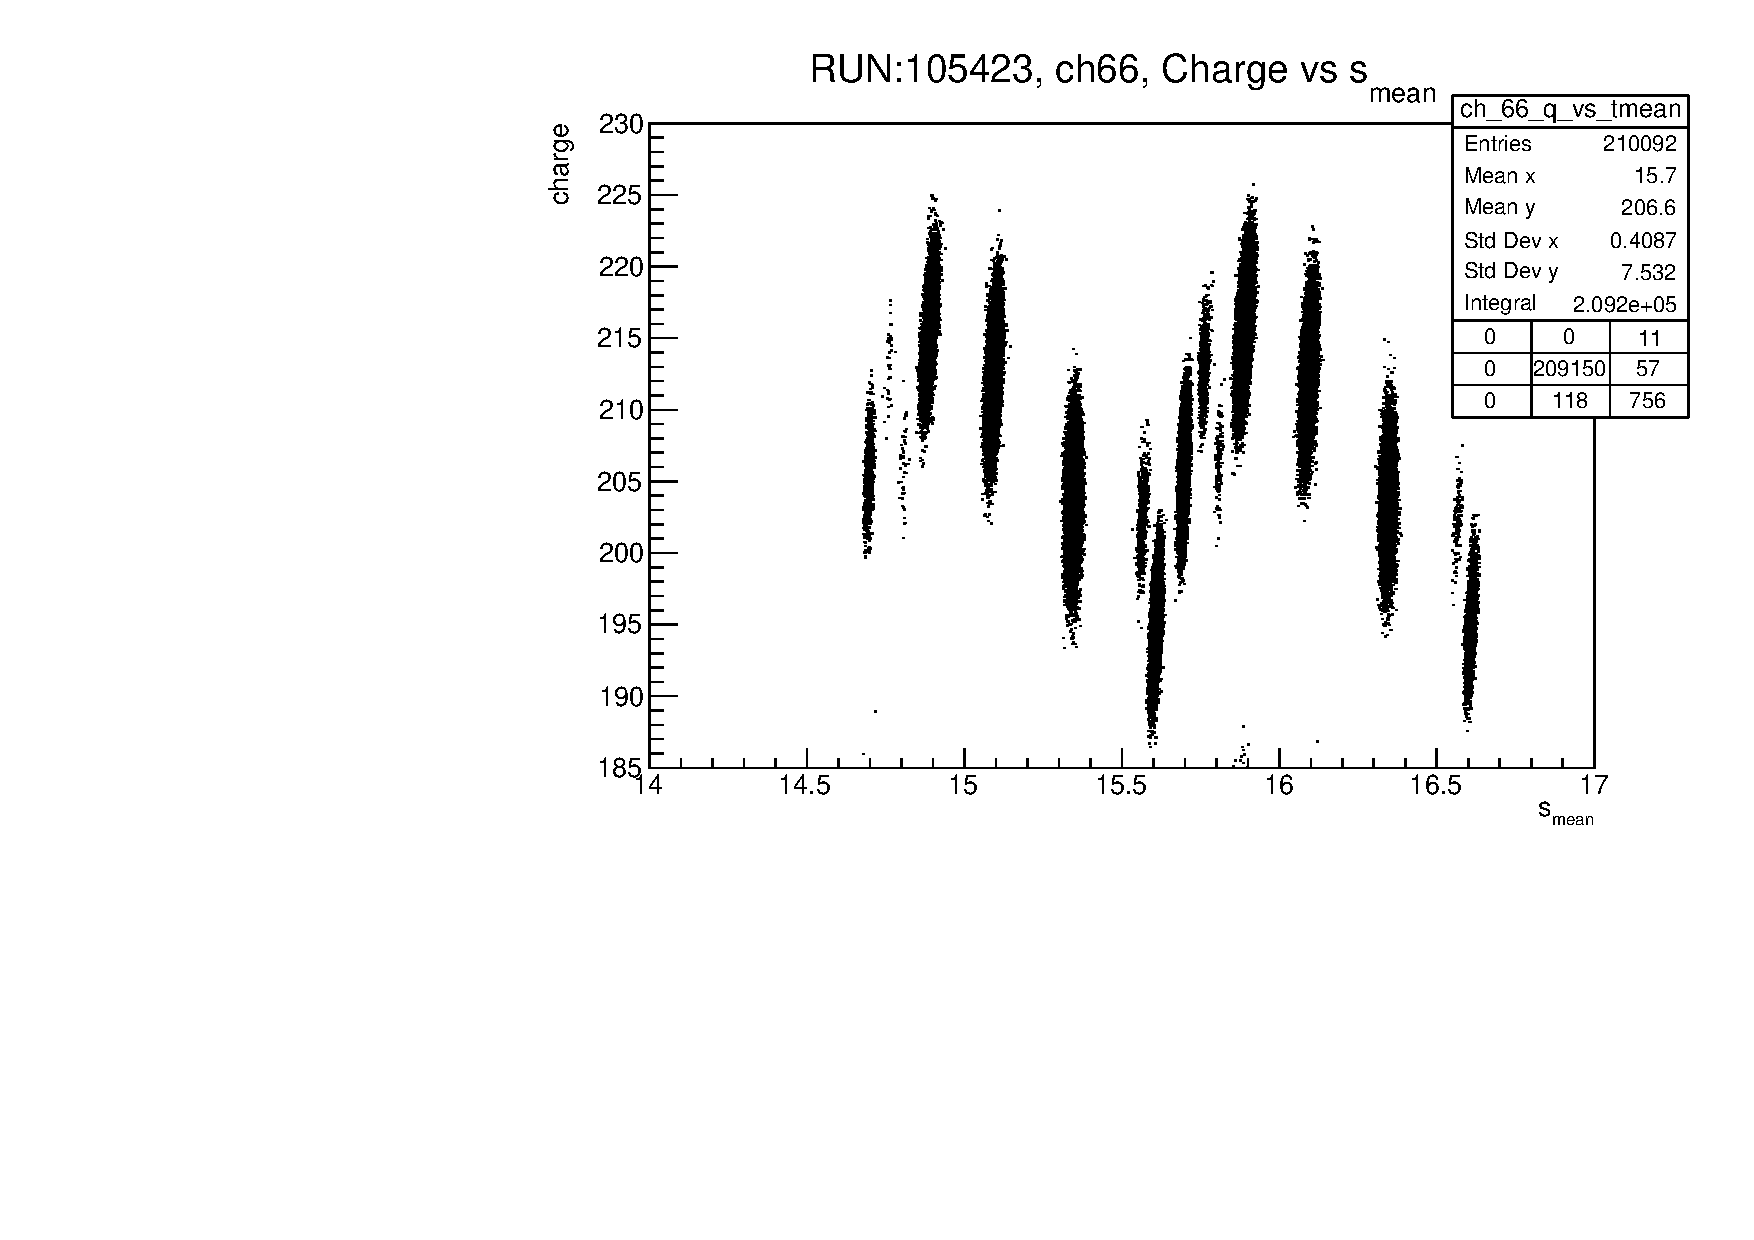
\includegraphics[width=0.65\textwidth]{figures/pdf/chtmean.pdf}
  \caption{2D histogram of $s_{mean}$ ($x$-axis) versus charge ($y$-axis).}
  \label{fig:chtm}
\end{figure}
\begin{figure}[!h]
  \centering
  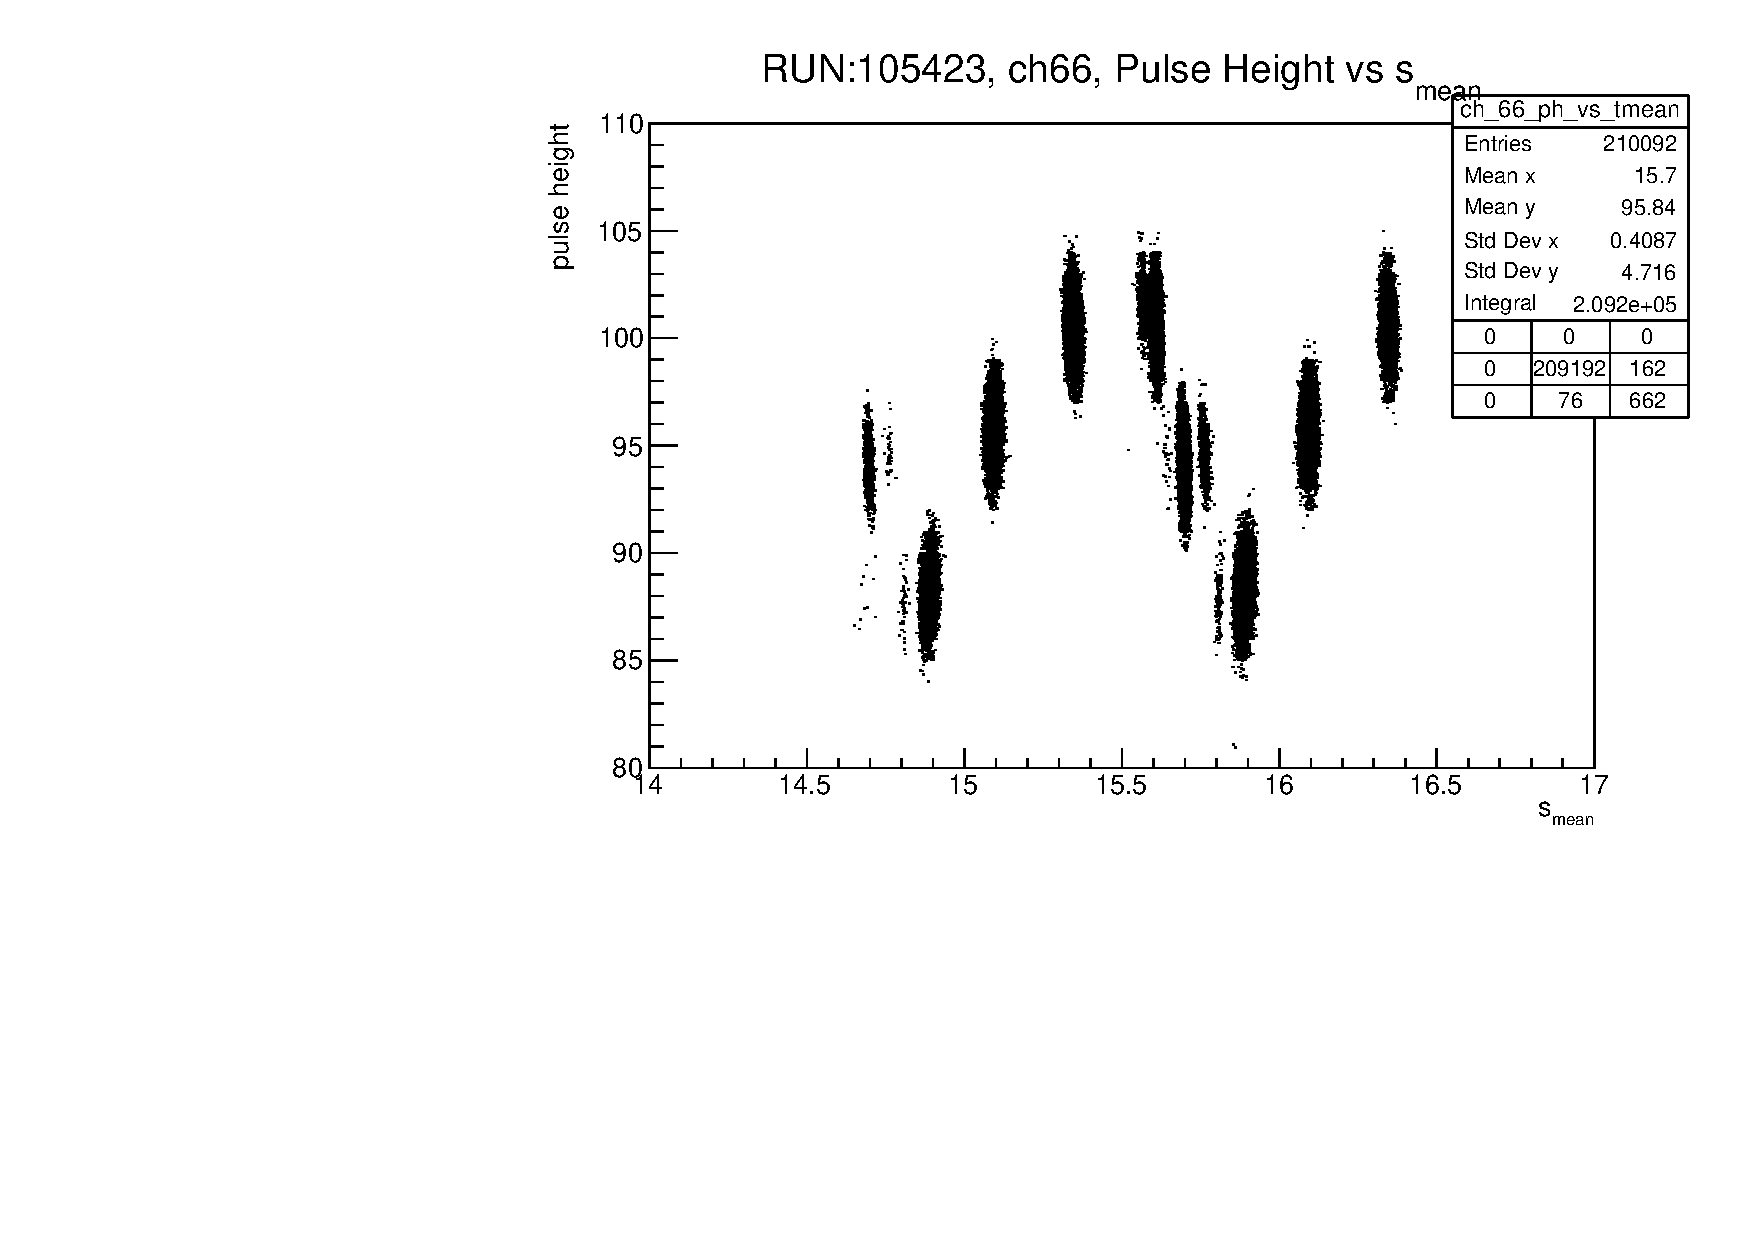
\includegraphics[width=0.65\textwidth]{figures/pdf/phtmean1.pdf}
  \caption{2D histogram of $s_{mean}$ ($x$-axis) versus pulse height ($y$-axis).}
  \label{fig:phtm}
\end{figure}
The pulse height and charge peaks are perfectly correlated with the $s_{mean}$ peaks. 
In particular, few ns of delay between waveforms, correlated with the ADC clock, 
result in three or two peaks in the charge and pulse height distribution. 
These peaks are merely artifacts of the pulser timing shifted with respect to the ADC 
clock and are not problematic. This behaviour was also confirmed with a simple simulation.
The simulation generates two series of triangular pulses, each delayed with respect to the other and models the behaviour 
of the corresponding ADC outputs. The ADC is simulated by partitioning signals into bins and calculating the signal mean within each bin. 
The delay between the two series is shorter than the width of the ADC bins. The output of the simulated ADC consists of square waves 
for each series of triangular pulses. The integrals and maximum values of the square waves over defined intervals are then computed.
The result is shown in Figure \ref{fig:simsim}. The simulation is not intended to replicate reality in its entirety, 
but rather serves as a tool for understanding the correlation between the ADC clock and pulser timing. 
While the simulated charge and pulse height distributions effectively exhibit peaks, they do not precisely 
match the number of peaks seen in Figure \ref{fig:ch1} and \ref{fig:ph2}. Since the ADC begins integration 
at the same time for both pulse series, any temporal shift between waves results in lower or greater waveform values on the 
$y$-axis at identical times. This discrepancy translates into distinct ADC outputs and consequently affects the observed pulse height. 
The same principle applies to the charge. Furthermore, the pulse height peaks exhibit clear distinctions with respect to the charge ones, 
a characteristic also evident in Figure \ref{fig:ch1} and \ref{fig:ph2}.
\begin{figure}[!h]
  \centering
  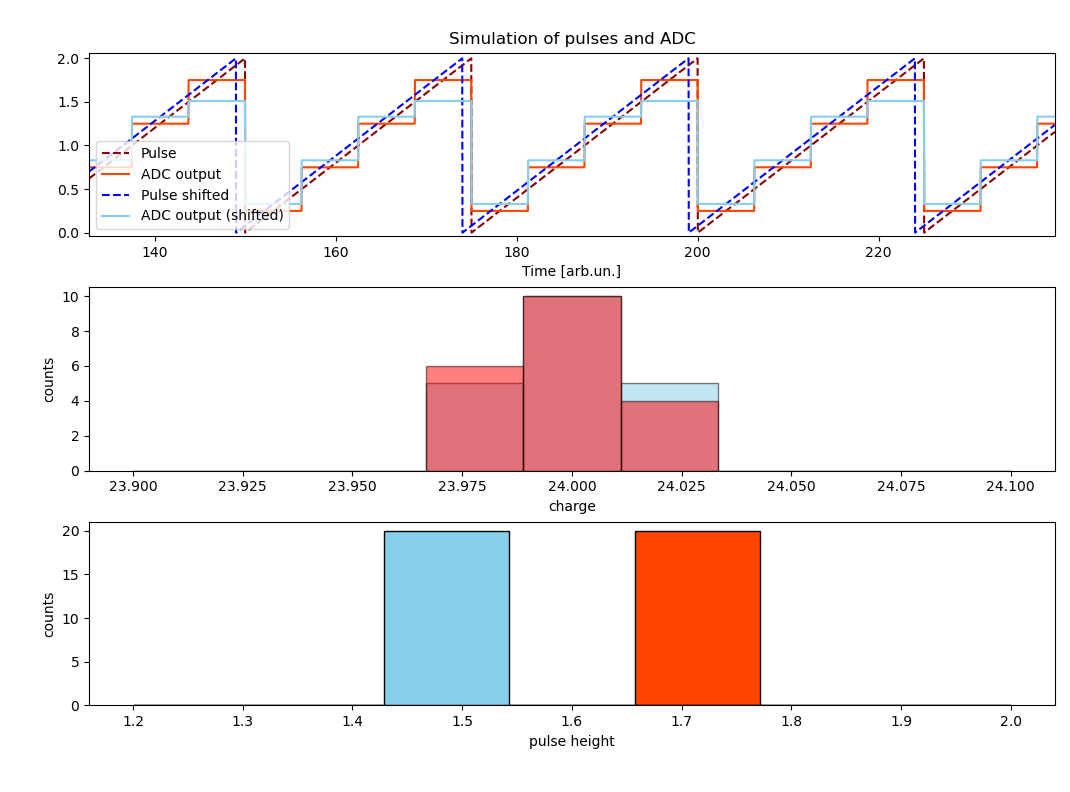
\includegraphics[width=0.85\textwidth]{figures/png/pres.png}
  \caption{Simulation of charge and pulse height distribution behaviour. 
  In the upper plot, triangular pulses representing charge injection waveforms are 
  plotted alongside the square waves from the simulated ADC. The red wave corresponds to the dark red pulses, 
  while the light blue wave corresponds to the dark blue pulses, shifted from the red one. In the central plot, 
  the distribution of charge is displayed, and in the bottom plot, the distribution of pulse height is shown. 
  The light blue distribution corresponds to the light blue ADC, and the same goes for the red one.}
  \label{fig:simsim}
\end{figure}
Lower values of pulse height or charge correspond to inverted waveforms, as mentioned in Sections \ref{nhitvschid} and \ref{wf}, 
or to glitches. In the case of inverted waveforms, the charge value was $\sim$100 and the pulse height $\sim$20, while for glitches, $\lesssim$70 and $\sim$35. 
An example of a glitch is shown in Figure \ref{fig:glitches}. The origin of the glitches is not yet understood.
\begin{figure}[!h]
  \centering
  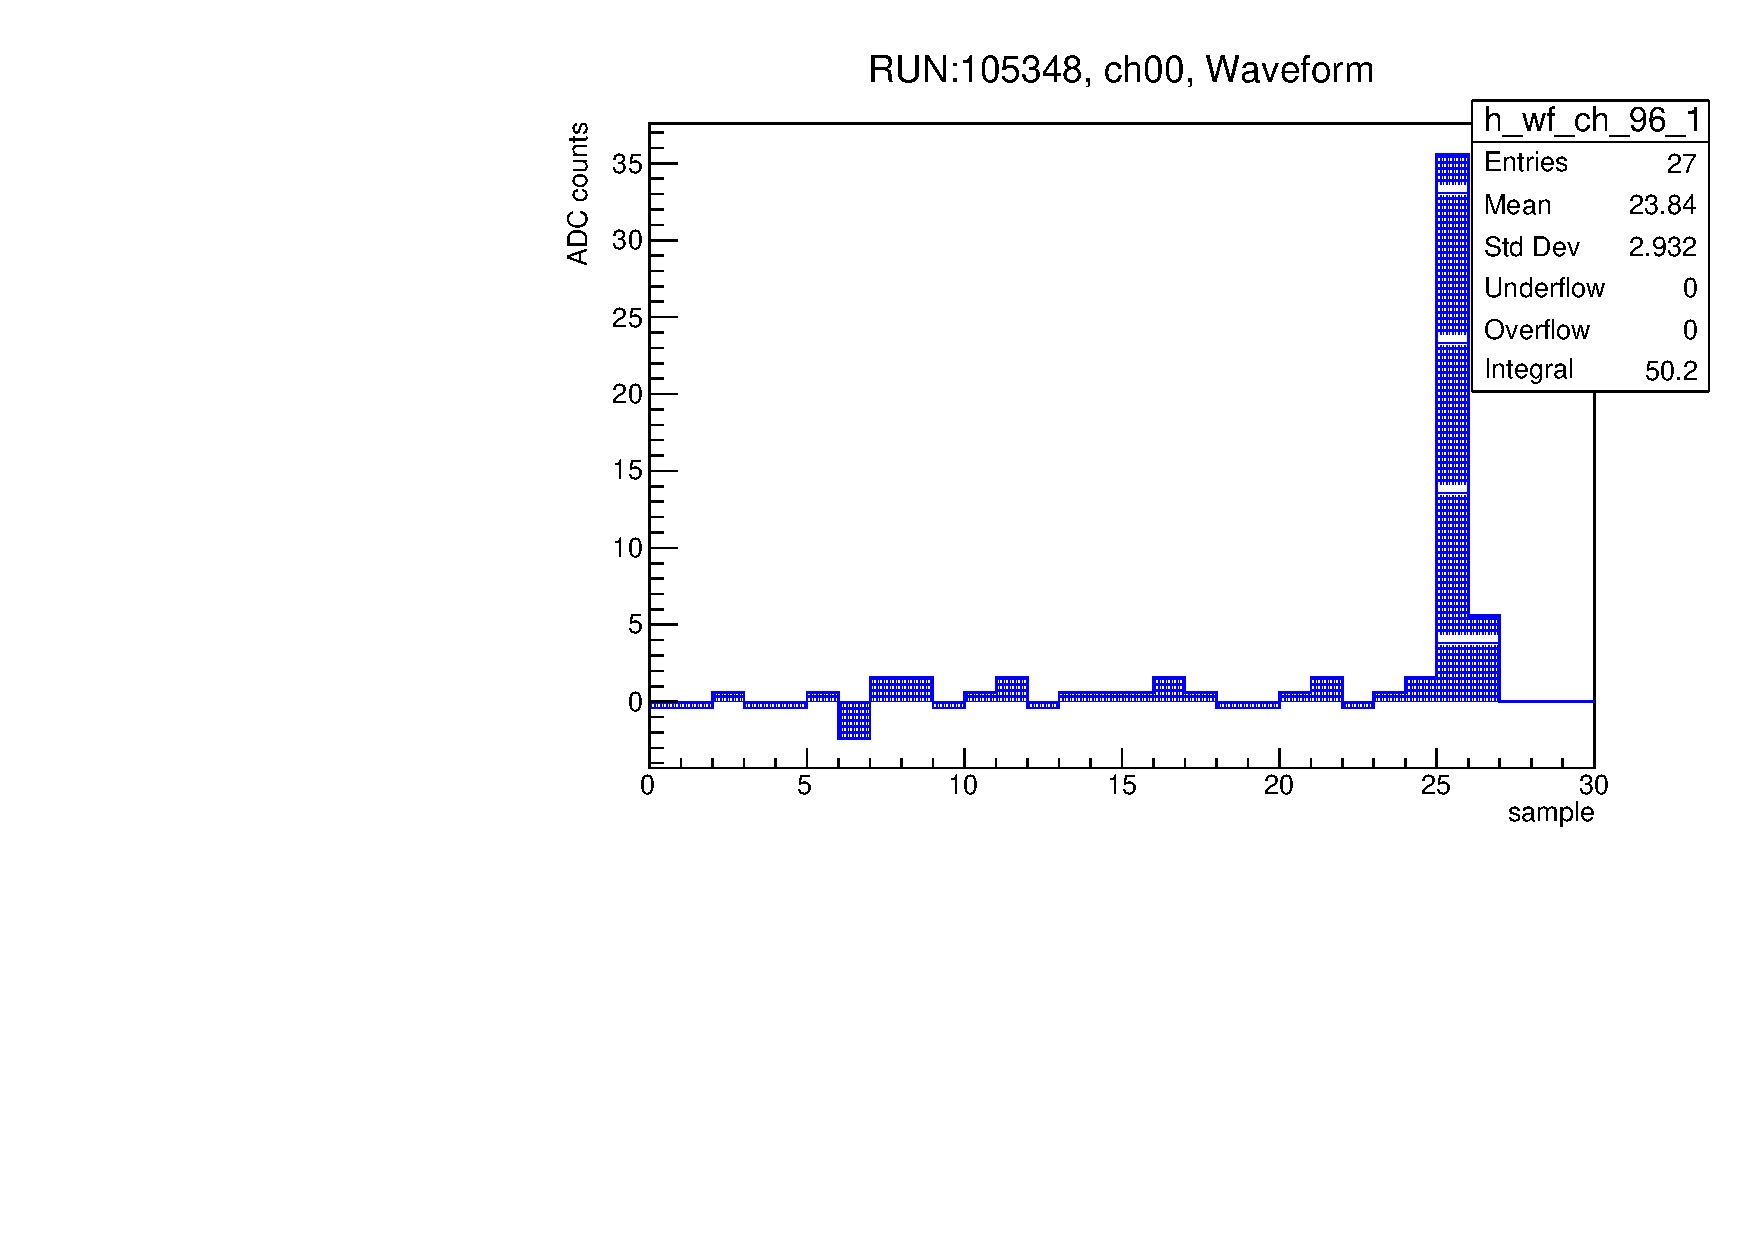
\includegraphics[width=0.65\textwidth]{figures/pdf/glitch.pdf}
  \caption{Glitch waveform of channel 0.}
  \label{fig:glitches}
\end{figure}
Special channels with excessive noise were identified through the charge distribution. 
Figure \ref{fig:noisywf} shows an example of a noisy waveform. 
Since the threshold mentioned in Section \ref{threshold} is 5 ADC counts, charge values for these channels were consistently lower than expected (approximately 10). 
This is due to the fact that only the first sample above 5 was considered as the entire waveform.
To address the issue, the channel voltage threshold was either adjusted or the preamp was replaced.
\begin{figure}[!h]
  \centering
  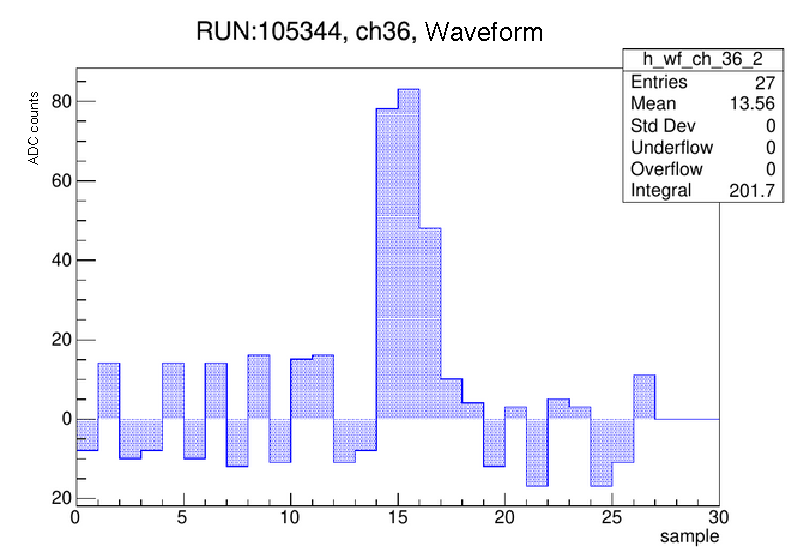
\includegraphics[width=0.65\textwidth]{figures/pdf/noise.pdf}
  \caption{Noisy waveform of the 36th channel.}
  \label{fig:noisywf}
\end{figure}

\subsubsection{Channels response uniformity}
In view of data taking, it was important to find an easy way to identify problematic channels and check the uniformity of channel responses. 
For this reason, plots of charge, first sample, pulse height and baseline means versus channel ID were produced. 
These plots are shown in Figures \ref{fig:means}. 
The outliers in the plots are due to crosstalk, noisy channels, inverted waveforms and glitches.
\begin{figure}[!h]
  \centering
  \begin{subfigure}[t]{0.5\textwidth}
      \centering
      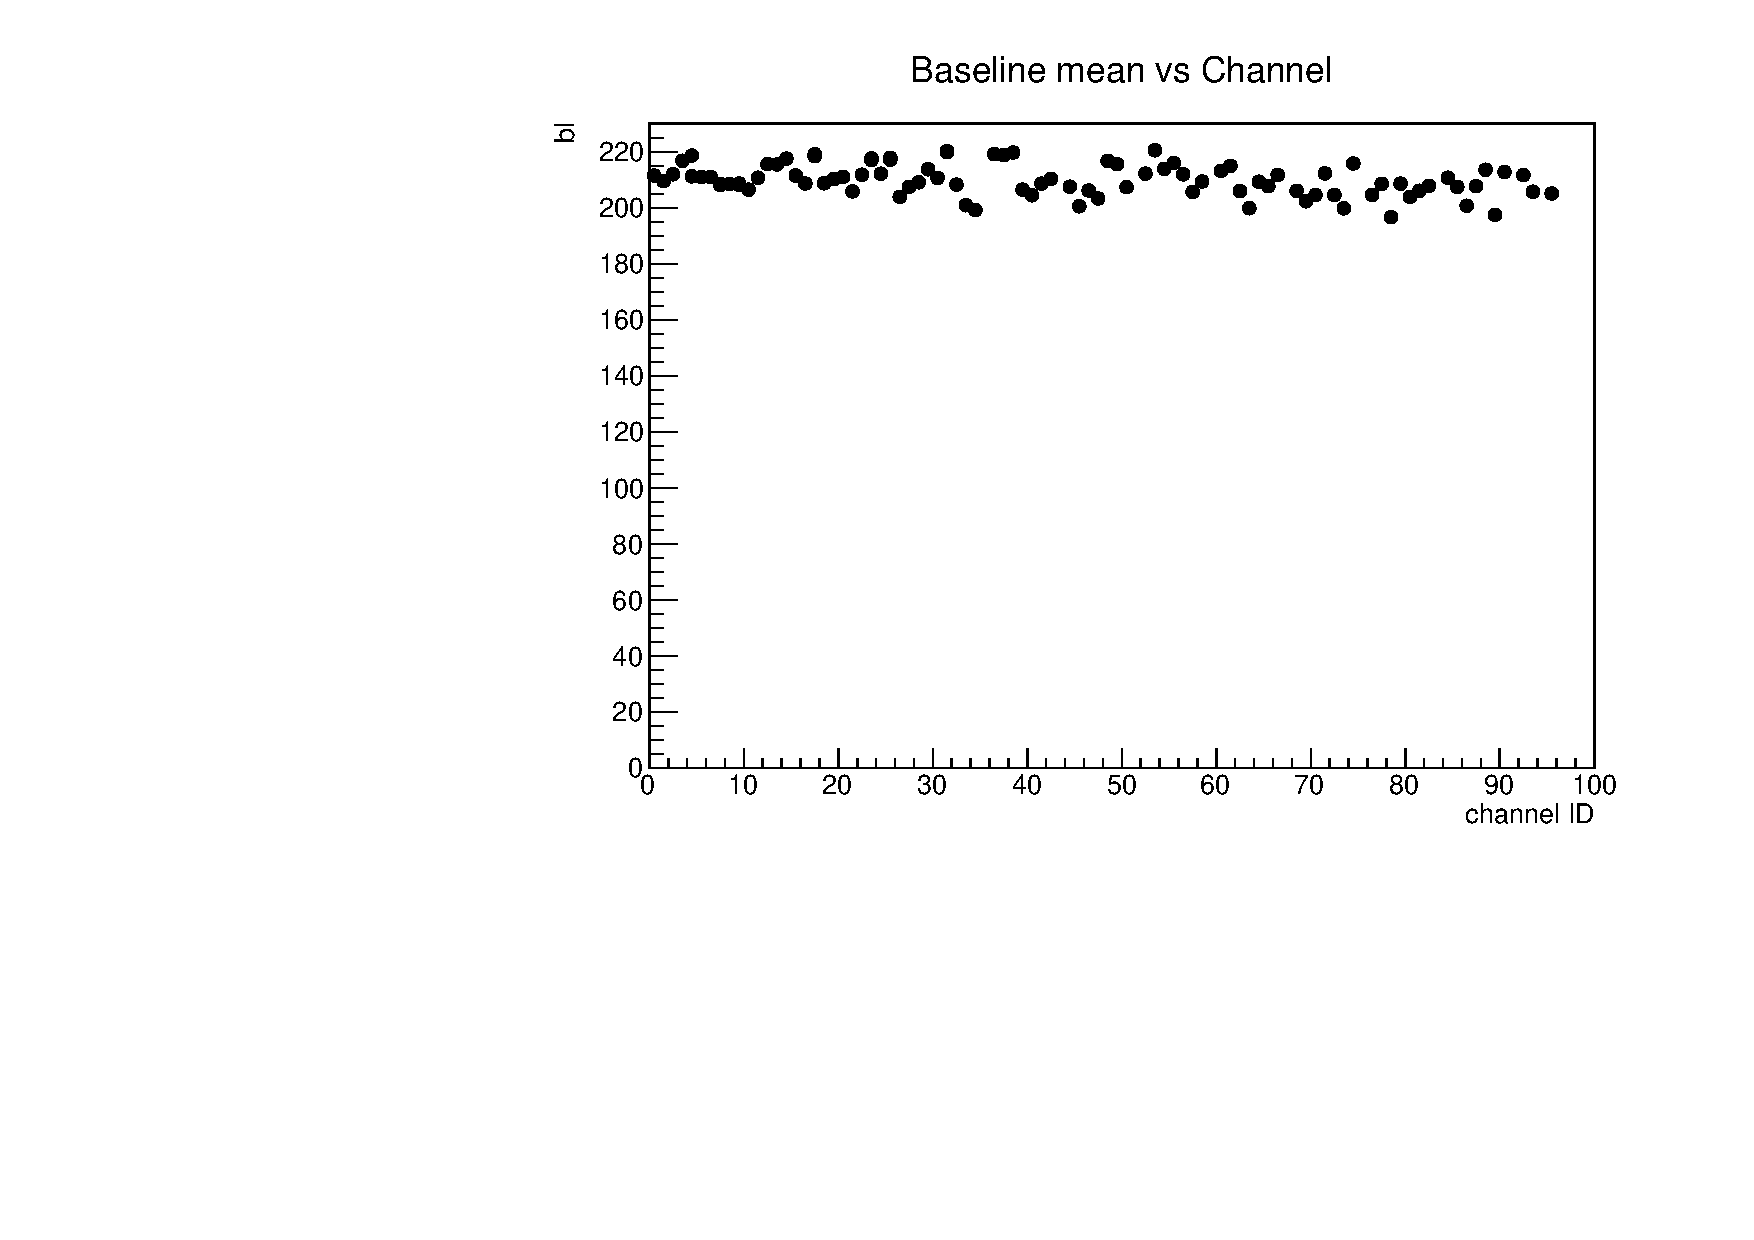
\includegraphics[width=\textwidth]{figures/pdf/bl_vs_ch1.pdf}
      \caption{}
  \end{subfigure}%
  ~ 
  \begin{subfigure}[t]{0.5\textwidth}
      \centering
      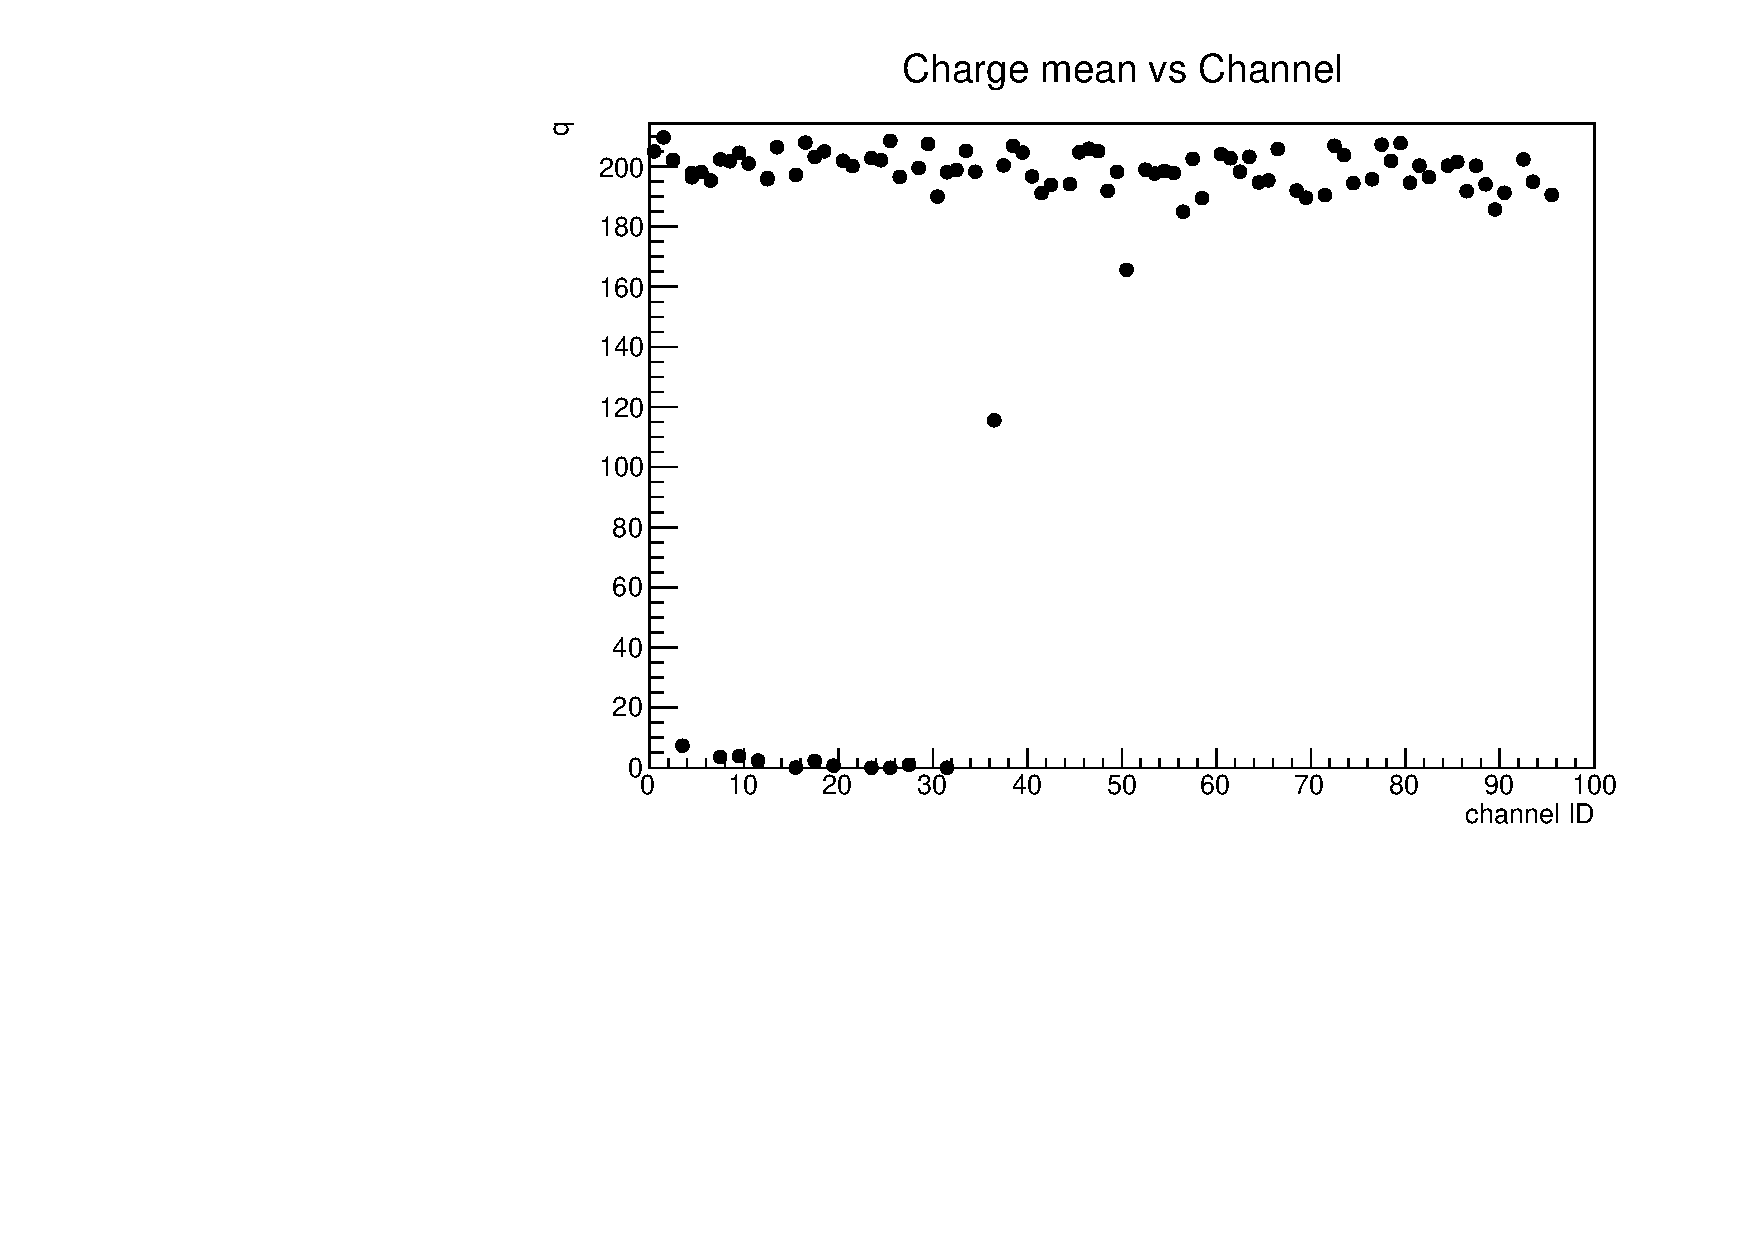
\includegraphics[width=\textwidth]{figures/pdf/q_vs_ch1.pdf}
      \caption{}
  \end{subfigure}
  ~ 
  \begin{subfigure}[t]{0.5\textwidth}
    \centering
    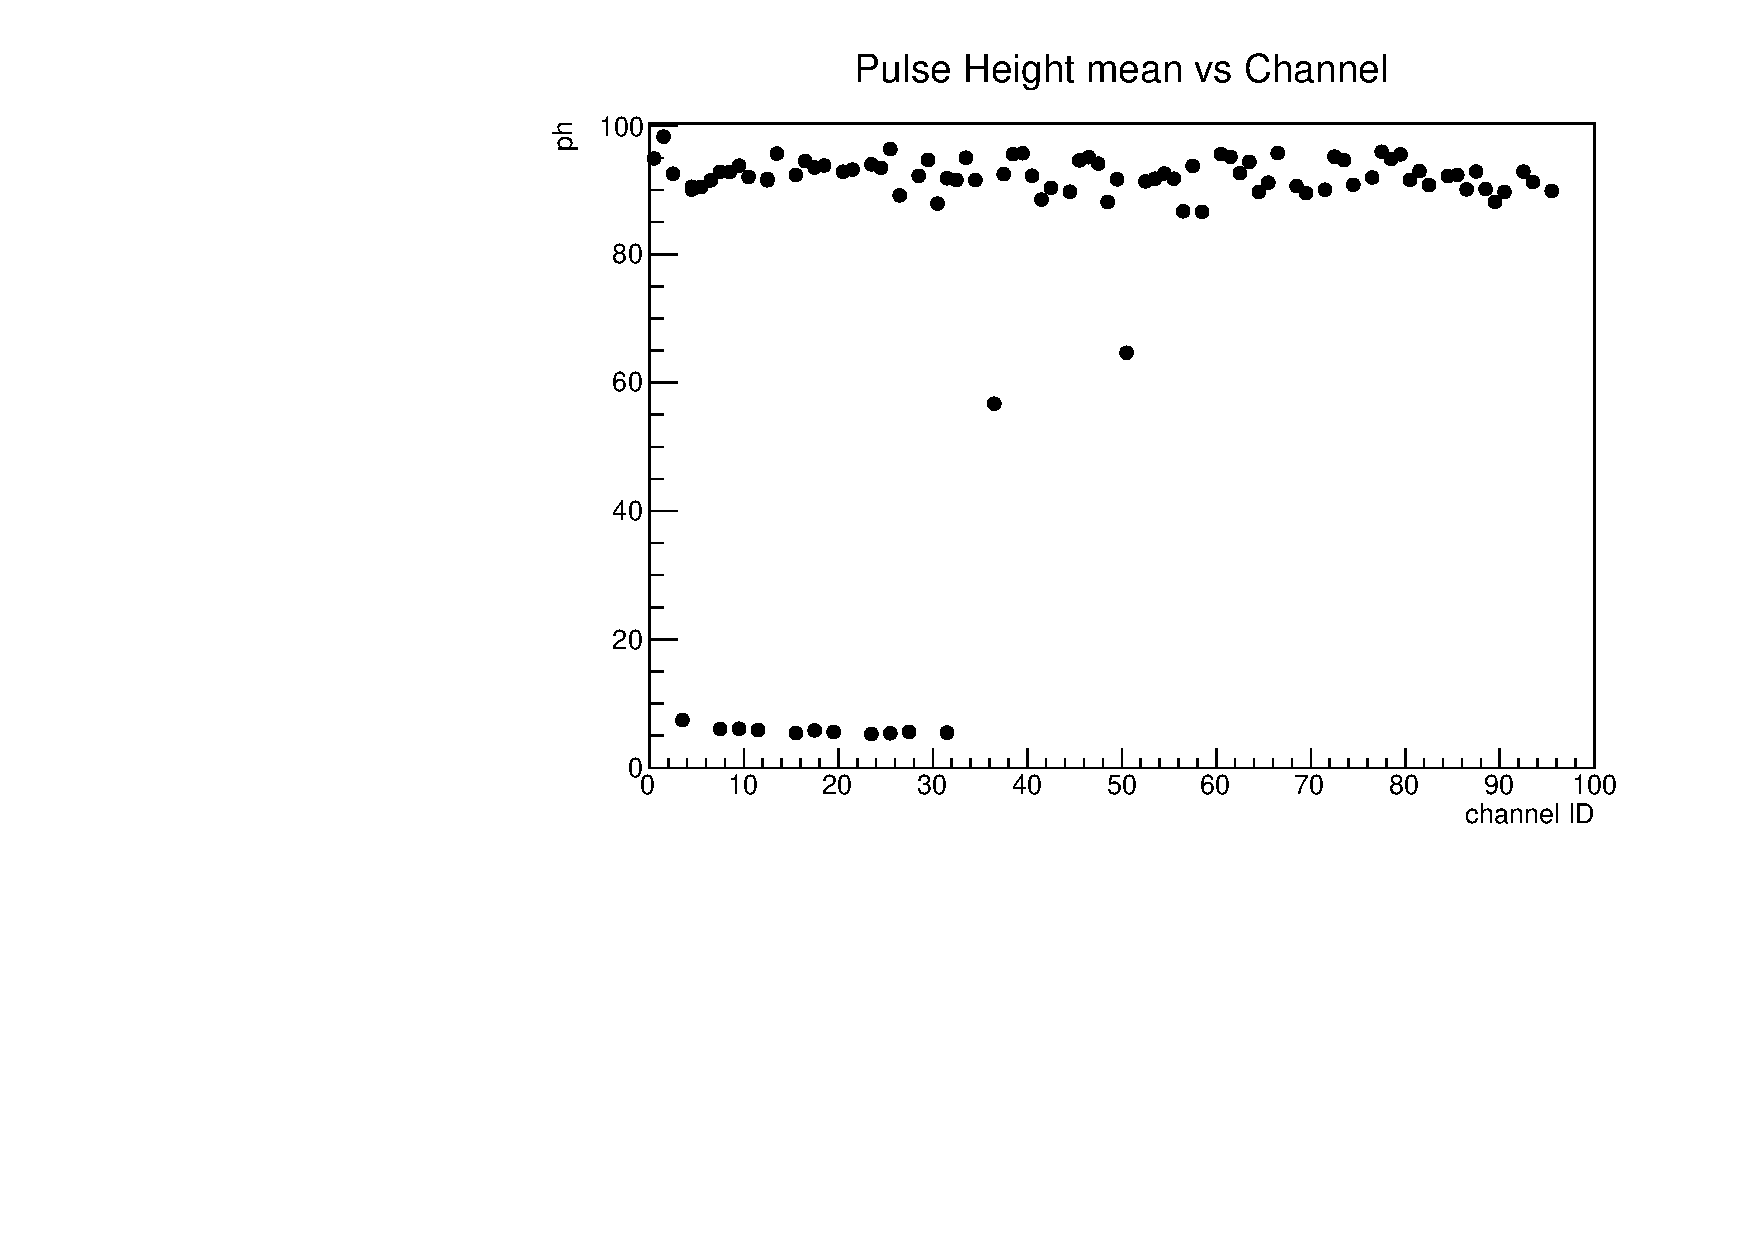
\includegraphics[width=\textwidth]{figures/pdf/ph_vs_ch1.pdf}
    \caption{}
\end{subfigure}%
~ 
\begin{subfigure}[t]{0.5\textwidth}
    \centering
    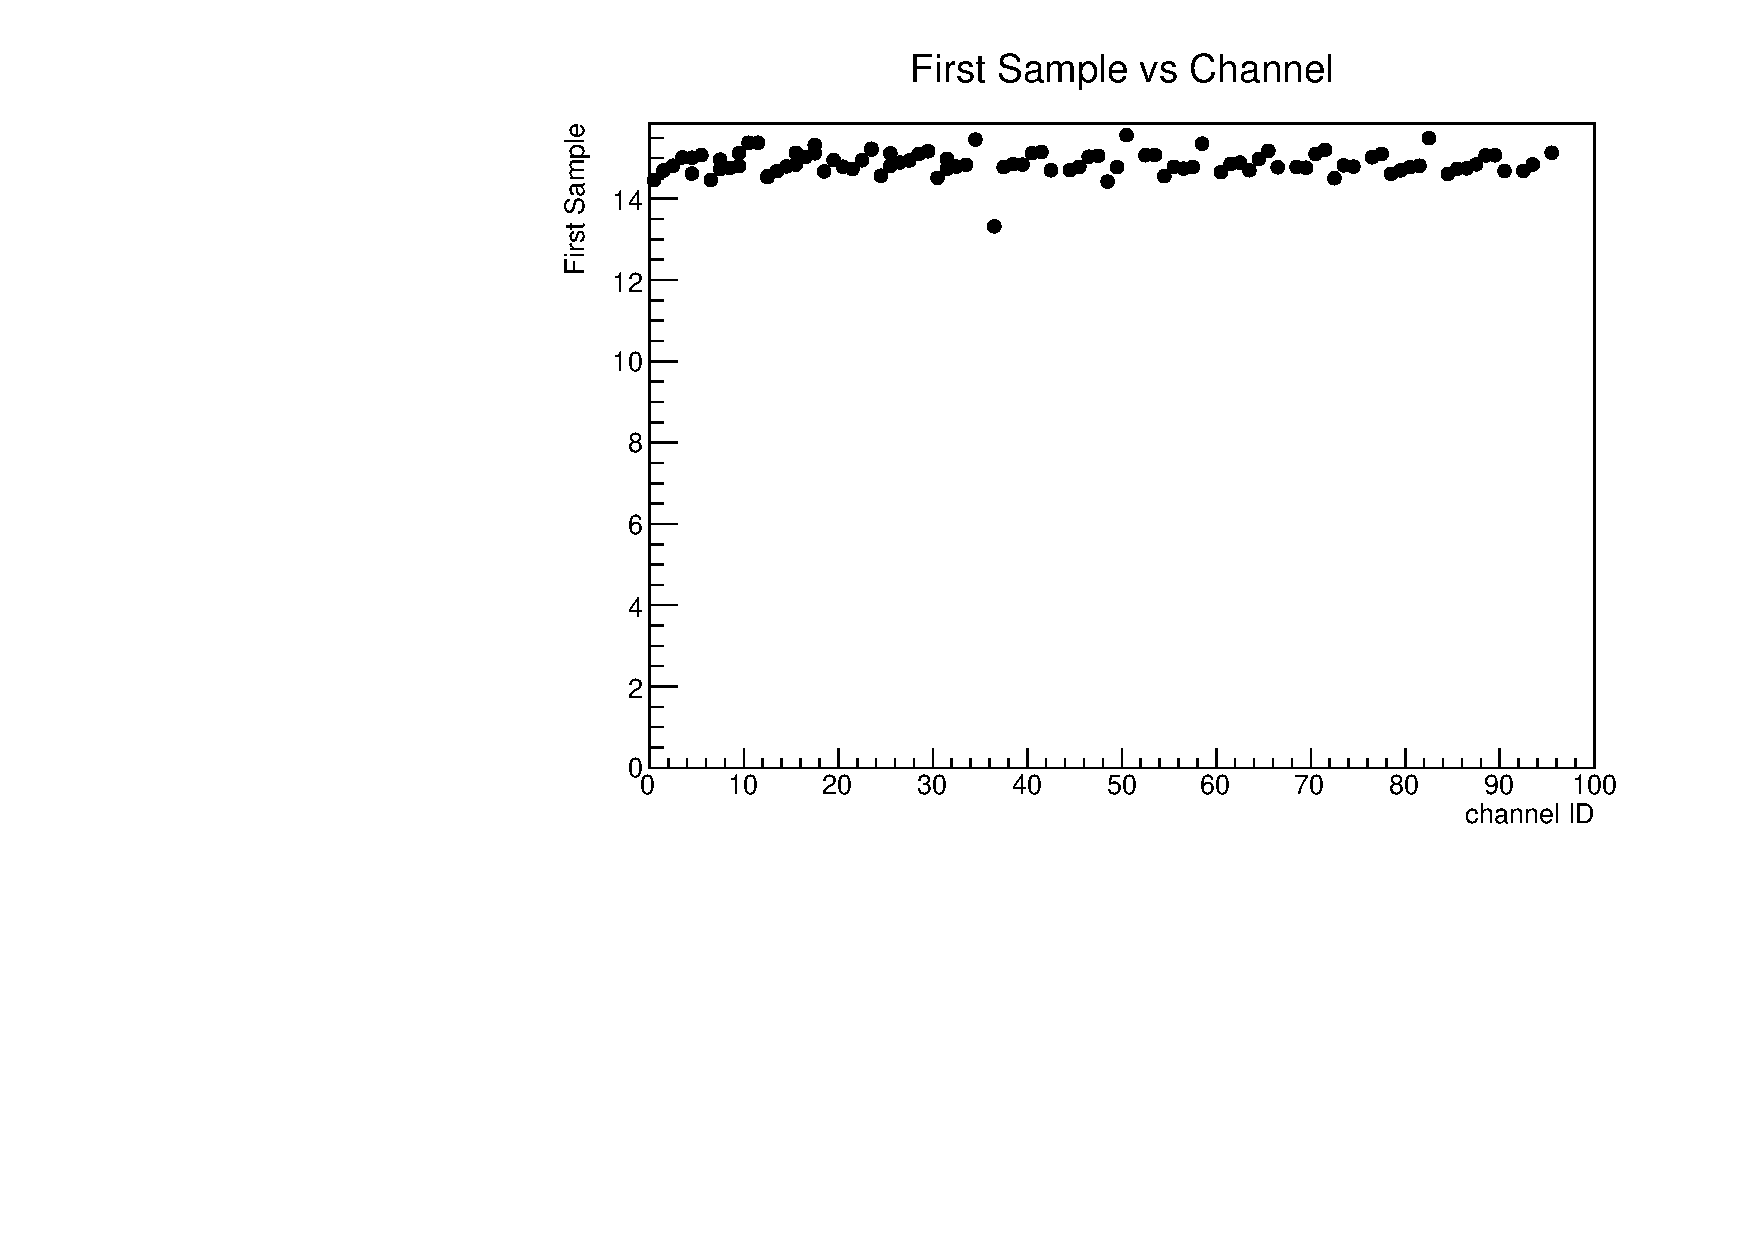
\includegraphics[width=\textwidth]{figures/pdf/fs_vs_ch1.pdf}
    \caption{}
\end{subfigure}
  \caption{Baseline (a), charge (b), pulse height (c), first sample (d) mean value versus channel ID.}
  \label{fig:means}
\end{figure}

\section{DAQ performance studies with external CFO}
The brief and straightforward test described in this section uses the CFO in a mode expected to be 
implemented during data acquisition. 
In the test, sequences of HBs \ref{des} separated by a time constant  
\( T_0 \) were generated and sent to the DTC. The test procedure was fully programmable. 
The \textit{run plan} was written using a simple, basic-like language, 
compiled, loaded into the CFO, and executed. This approach covers nearly 
all conceivable use cases. We operated in two distinct modes:
\begin{itemize}
  \item \textit{Emulated CFO} mode: the DTC generates HBs and 
  EWMs \ref{tdaqtra} and reads one ROC;
  \item \textit{External CFO} mode: the CFO generates HBs and 
  EWMs, sends them to the DTC, and the DTC reads the ROC.
\end{itemize}
Both DTC and CFO were installed in the DAQ computer mu2edaq09. 
The block diagram scheme is similar to the one shown in Figure \ref{fig:blockdiagram}, 
with the exception of the CFO and DTC blocks (Figure \ref{fig:secondtest}).
In both modes, the CFO (or the DTC, in the \textit{emulated CFO} mode) 
sends a sequence of \( (N+1) \) EWMs. Afterward, the DTC 
asynchronously reads \( N \) events. 
Time synchronization between the CFO, DTCs, and ROCs was managed either 
internally (using FPGA) or with an external clock. 
The test setup involved two FPGAs - one acting as the CFO and 
one as the DTC - and one tracker test stand (one ROC). 
We conducted short runs with \( N \) events, each EW lasting  1.7 $\mu$s. 

\begin{figure}[!h]
  \centering
  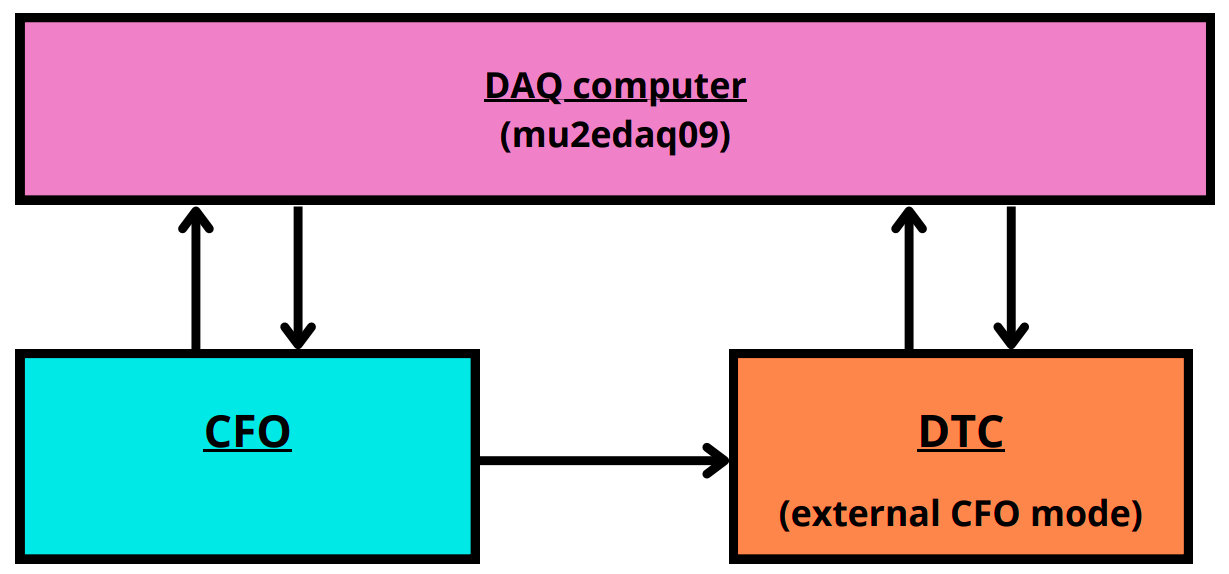
\includegraphics[width=0.65\textwidth]{figures/png/Screenshot_20240714_131546.png}
  \caption{The DTC and CFO block diagram 
  used for the DAQ performance studies with an external CFO.}
  \label{fig:secondtest}
\end{figure}



The output was analyzed, and the test was repeated multiple times to ensure reproducibility. 
My contribution to this test involved reading the data, whose format is shown in Figure \ref{fig:dataformat}, 
and comparing the number of events and status codes between runs with the same \textit{run plan}, 
both for \textit{emulated} and \textit{external CFO} mode. 
\begin{figure}[!h]
  \centering
  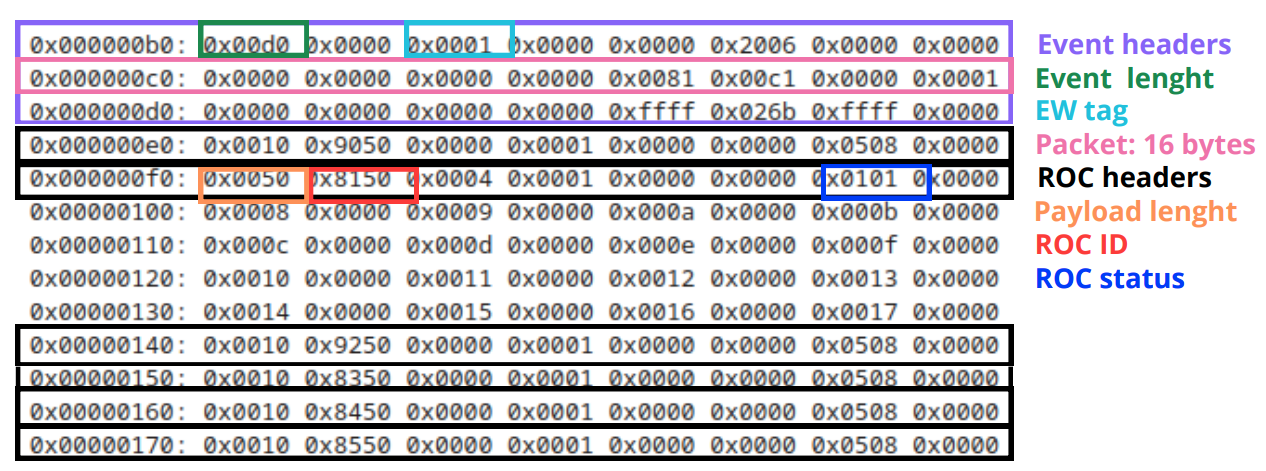
\includegraphics[width=\textwidth]{figures/png/Screenshot_20240628_104216.png}
  \caption{Each line (pink) in the data sequence is called \textit{data packet}. 
  The first three packets (grey) denote one event. The green and cyan squares represent respectively
  the number of packets in one event and the event window tag, which identifies a single event. 
  The following packets (black) represent the ROC headers, six in total, but just one ROC was connected. 
  The orange and red squares indicate the payload length (the number of packets after 
  the ROC header, including the ROC header) and the ROC ID respectively. The blue square represents 
  the ROC status. There are different status codes: 0x0101 indicates a full payload, 0x0100 an empty one, 
  and 0x0108, 0x0180, and 0x0508 are the codes for timeouts.}
  \label{fig:dataformat}
\end{figure}
Different \textit{run plans} were created, with different number of events generated in both modes:
\begin{itemize}
  \item \textit{External CFO} mode: the chosen number of generated 
  events per run was 66, 130, 258, 514, and 1026. These numbers 
  were chosen because we were reading out the events emulated by 
  the ROC, and the payload is fully defined by the EW tag. 
  It was possible to generate 64 different patterns, and the 
  first two patterns were easy to remember, seen at the end of each run. 
  Therefore, each time the number of events was doubled and 2 events were added at the end.
  \item \textit{Emulated CFO} mode: since it was the most stable mode, 
  it was decided to start with a greater number of events per run (10k and 100k).
\end{itemize}


The results for the \textit{emulated CFO} mode are shown in Figure 
\ref{fig:corruptionemulated}. This figure displays the total number of events, 
the number of empty (0x100) and full events (0x101), and the number of timeouts 
(0x108, 0x180, and 0x508) versus the run number per \textit{run plan}. We expect 
to see all events read out correctly, with just the presence of empty and full events 
as scheduled in the \textit{run plan}. This mode was much more stable compared to the 
\textit{external CFO} mode. As shown in the 10k events generated \textit{run plan} (Figure \ref{fig:corruptionemulated}(a)), 
the events are read out correctly, except for the 13th and the 19th runs. 
For the 100k \textit{run plan}, the majority of the events seem to be read out correctly, 
except for the 5th and 10th runs. It is possible to see a number of 0x0508 timeouts that is 
$10^{-3}$ the total number of events in most of the runs. This suggests the presence of a 
jitter with the external clock, indicating that the results depend on the source of timing synchronization.


\begin{figure}[!h]
  \centering
  \begin{subfigure}[t]{0.5\textwidth}
      \centering
      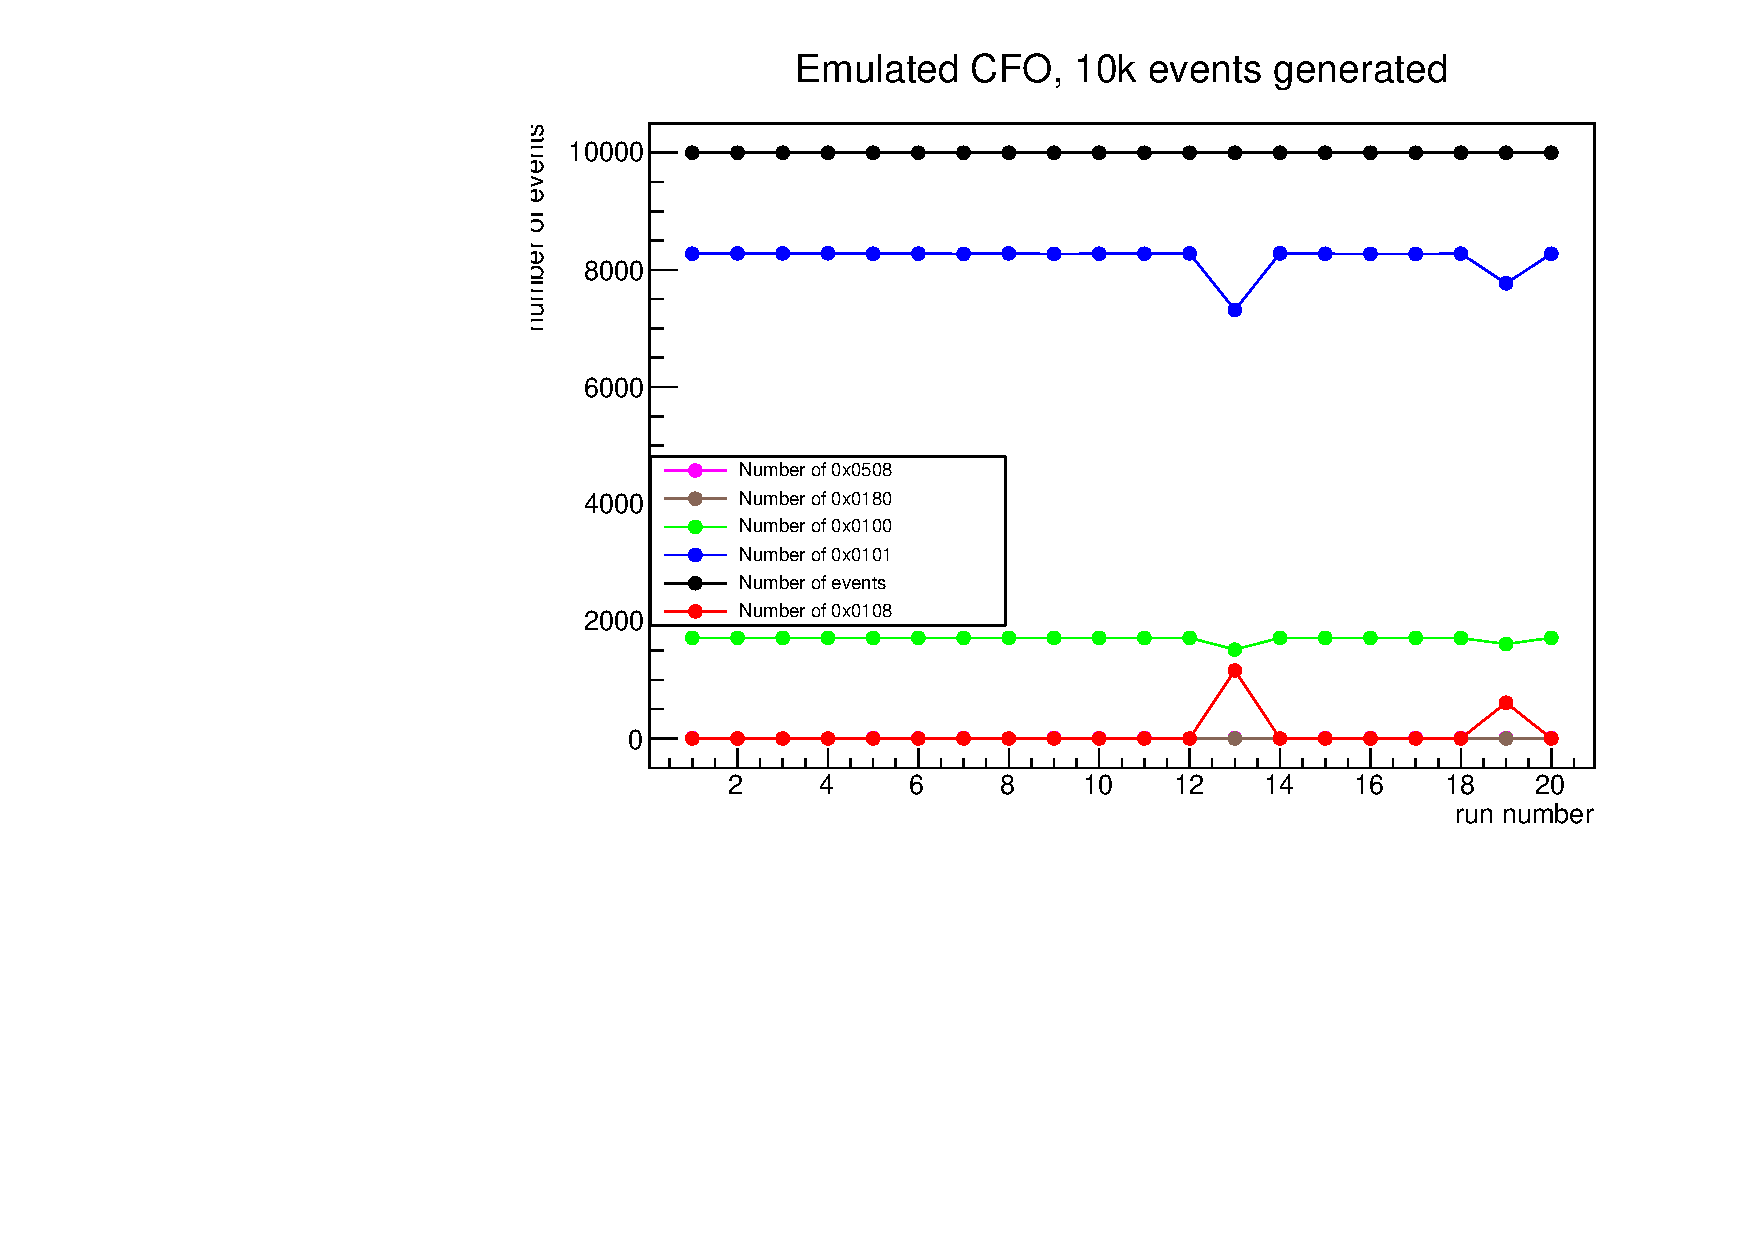
\includegraphics[width=1.1\textwidth]{figures/pdf/10k.pdf}
      \caption{}
  \end{subfigure}%
  ~ 
  \begin{subfigure}[t]{0.5\textwidth}
      \centering
      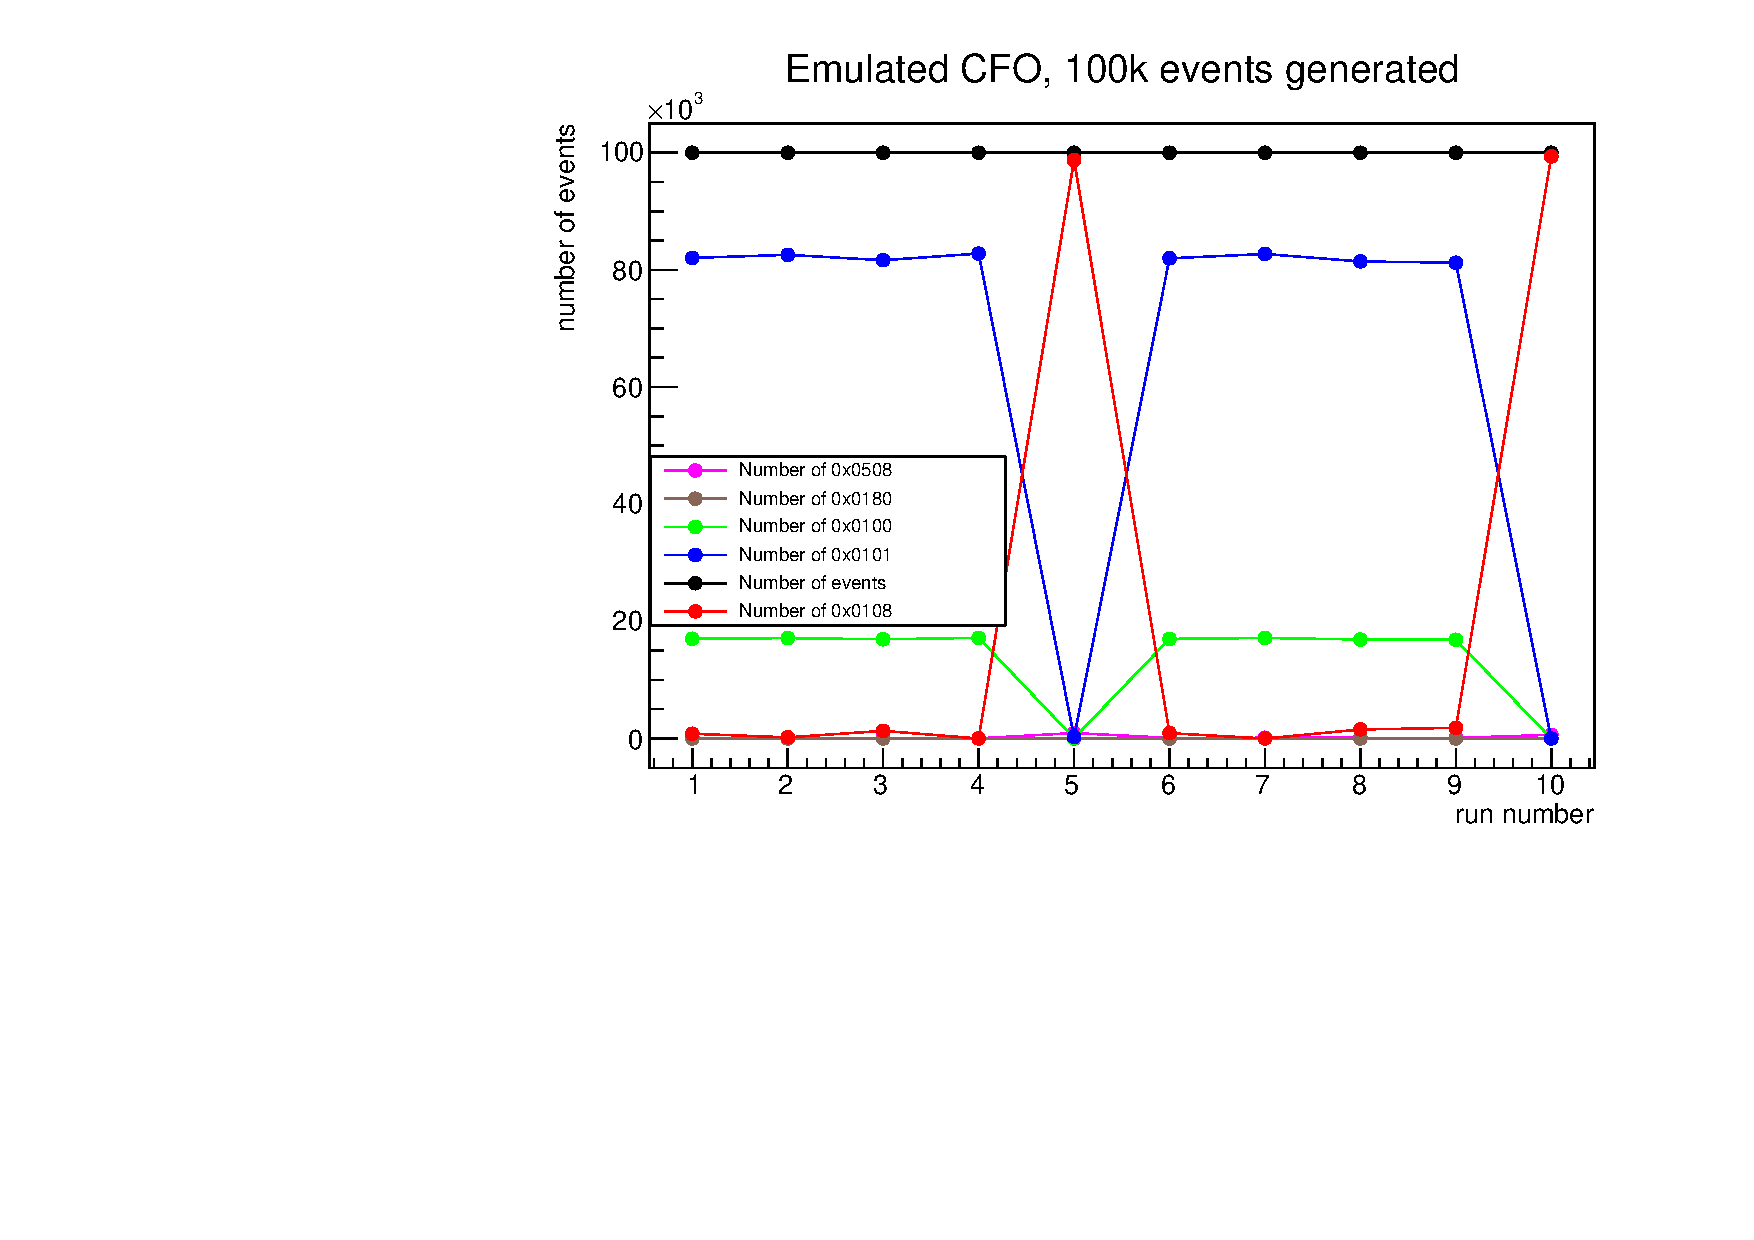
\includegraphics[width=1.1\textwidth]{figures/pdf/100k.pdf}
      \caption{}
  \end{subfigure}
  \caption{The \textit{emulated CFO} mode. Subfigures (a) and (b) show 10k and 100k events generated respectively. 
  The total number of events (black), the number of empty events (0x100 - green -) and full events (0x101 - blue -), 
  and the number of timeouts (0x108 - red -, 0x180 - brown -, and 0x508 - pink -) versus the run number in a \textit{run plan} are shown.
  }
  \label{fig:corruptionemulated}
\end{figure} 

The results for the \textit{external CFO} mode are shown in Figure \ref{fig:corruption}. 
These graphics show the total number of events, the number of empty (0x100) and full events (0x101), and 
the number of timeouts (0x108, 0x180, and 0x508) versus the run number per \textit{run plan}.
As can be seen in Figure \ref{fig:corruption}(a), all events are read out correctly, without any timeouts.
However, as the number of events generated increases, issues begin to arise.
In the cases of 130 and 258 events generated (Figures \ref{fig:corruption}(b) and (c)), only the first run 
was not read out correctly, resulting in only timeouts being read out.
Before starting the first run of the series, a new \textit{run plan} was uploaded, 
which suggests there may be an issue with the upload.
The case of 514 events (Figure \ref{fig:corruption}(d)) is different from the previous two: 
only the first run is read out correctly, ruling out previous assumptions. The main problem is 
that in the subsequent runs, approximately 60\% of the events are lost. Only the last events 
show up, and the first Event Window tag of the run is different from zero. The sum of the number 
of events read out and the first EW tag equals 514.
All events in the following runs appear to be timeouts. The same issue occurs with the 
1026 events generated case, where 30\% of events are lost.


\begin{figure}[!h]
  \centering
  \begin{subfigure}[t]{0.5\textwidth}
      \centering
      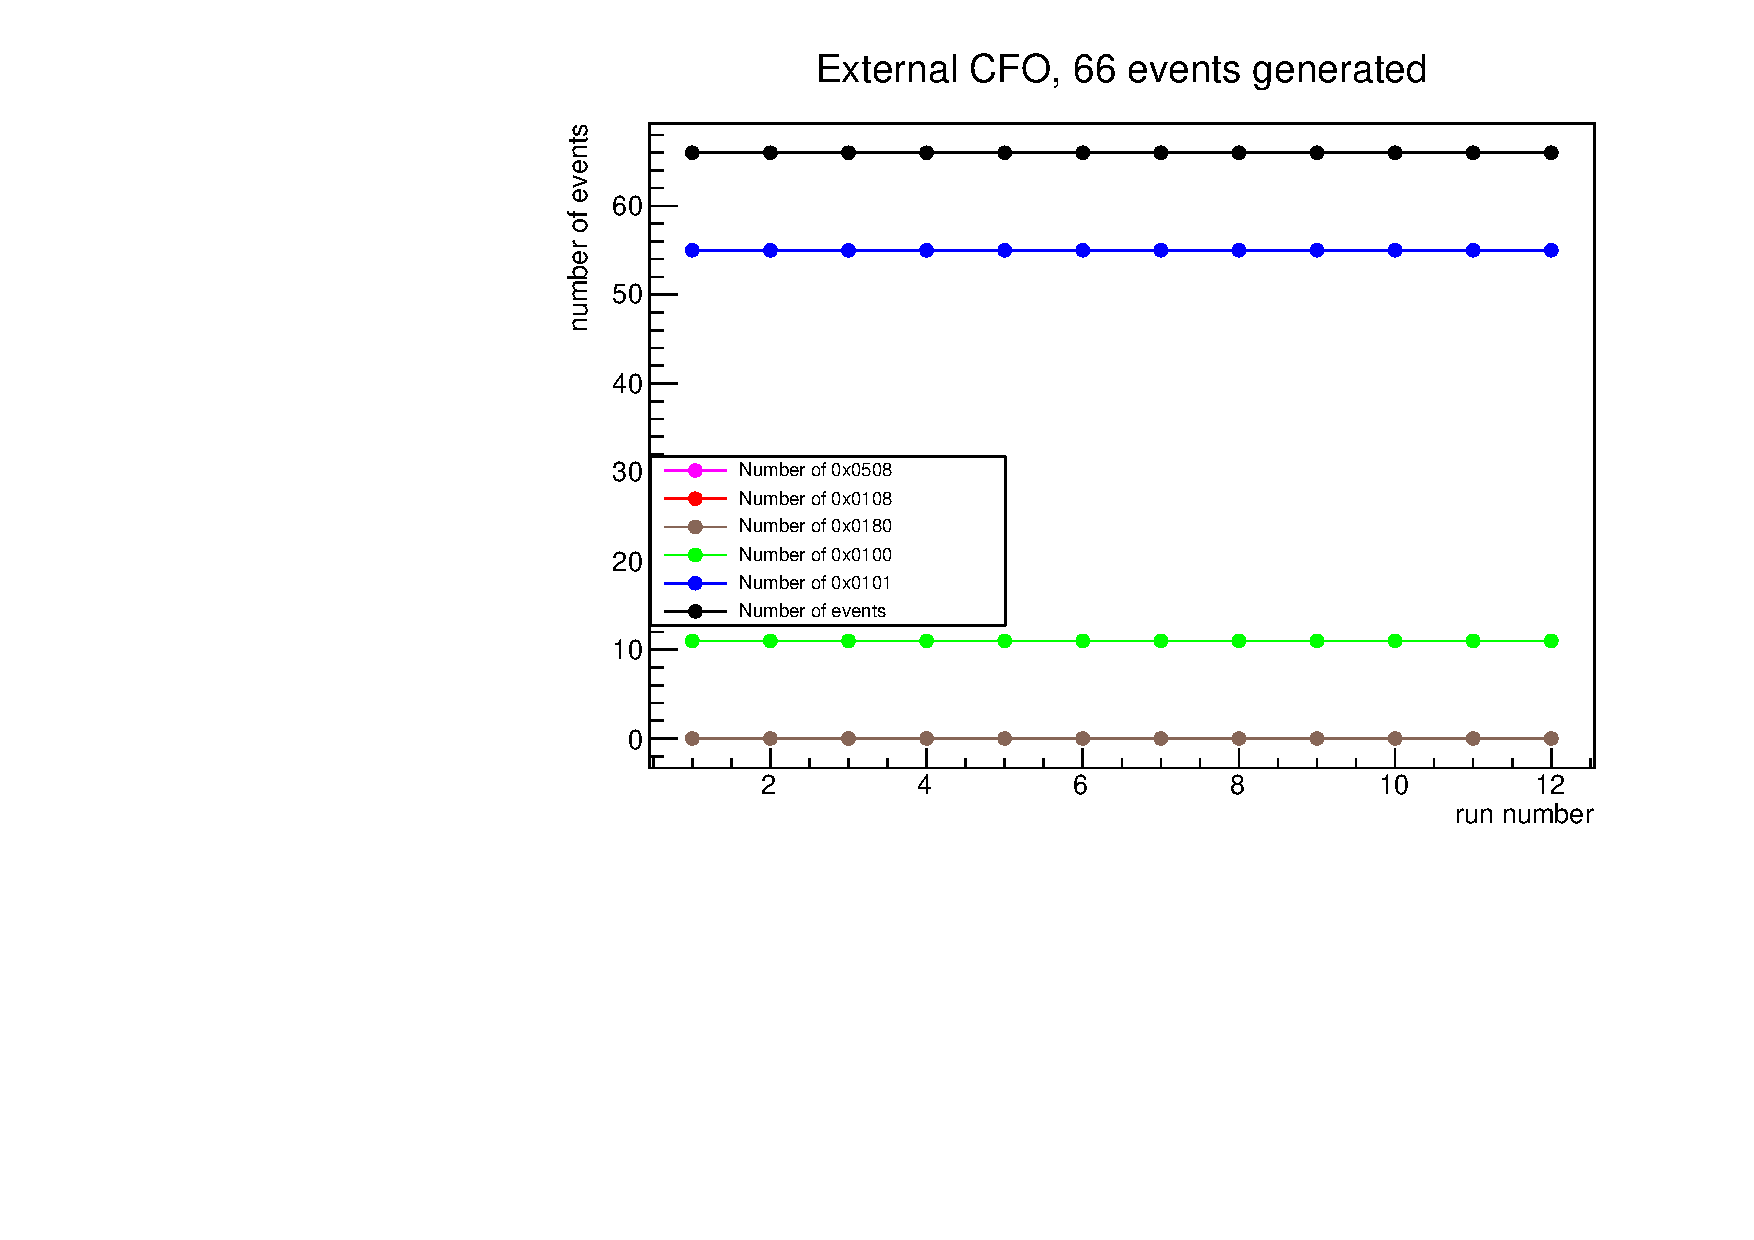
\includegraphics[width=1.1\textwidth]{figures/pdf/66.pdf}
      \caption{}
  \end{subfigure}%
  ~ 
  \begin{subfigure}[t]{0.5\textwidth}
      \centering
      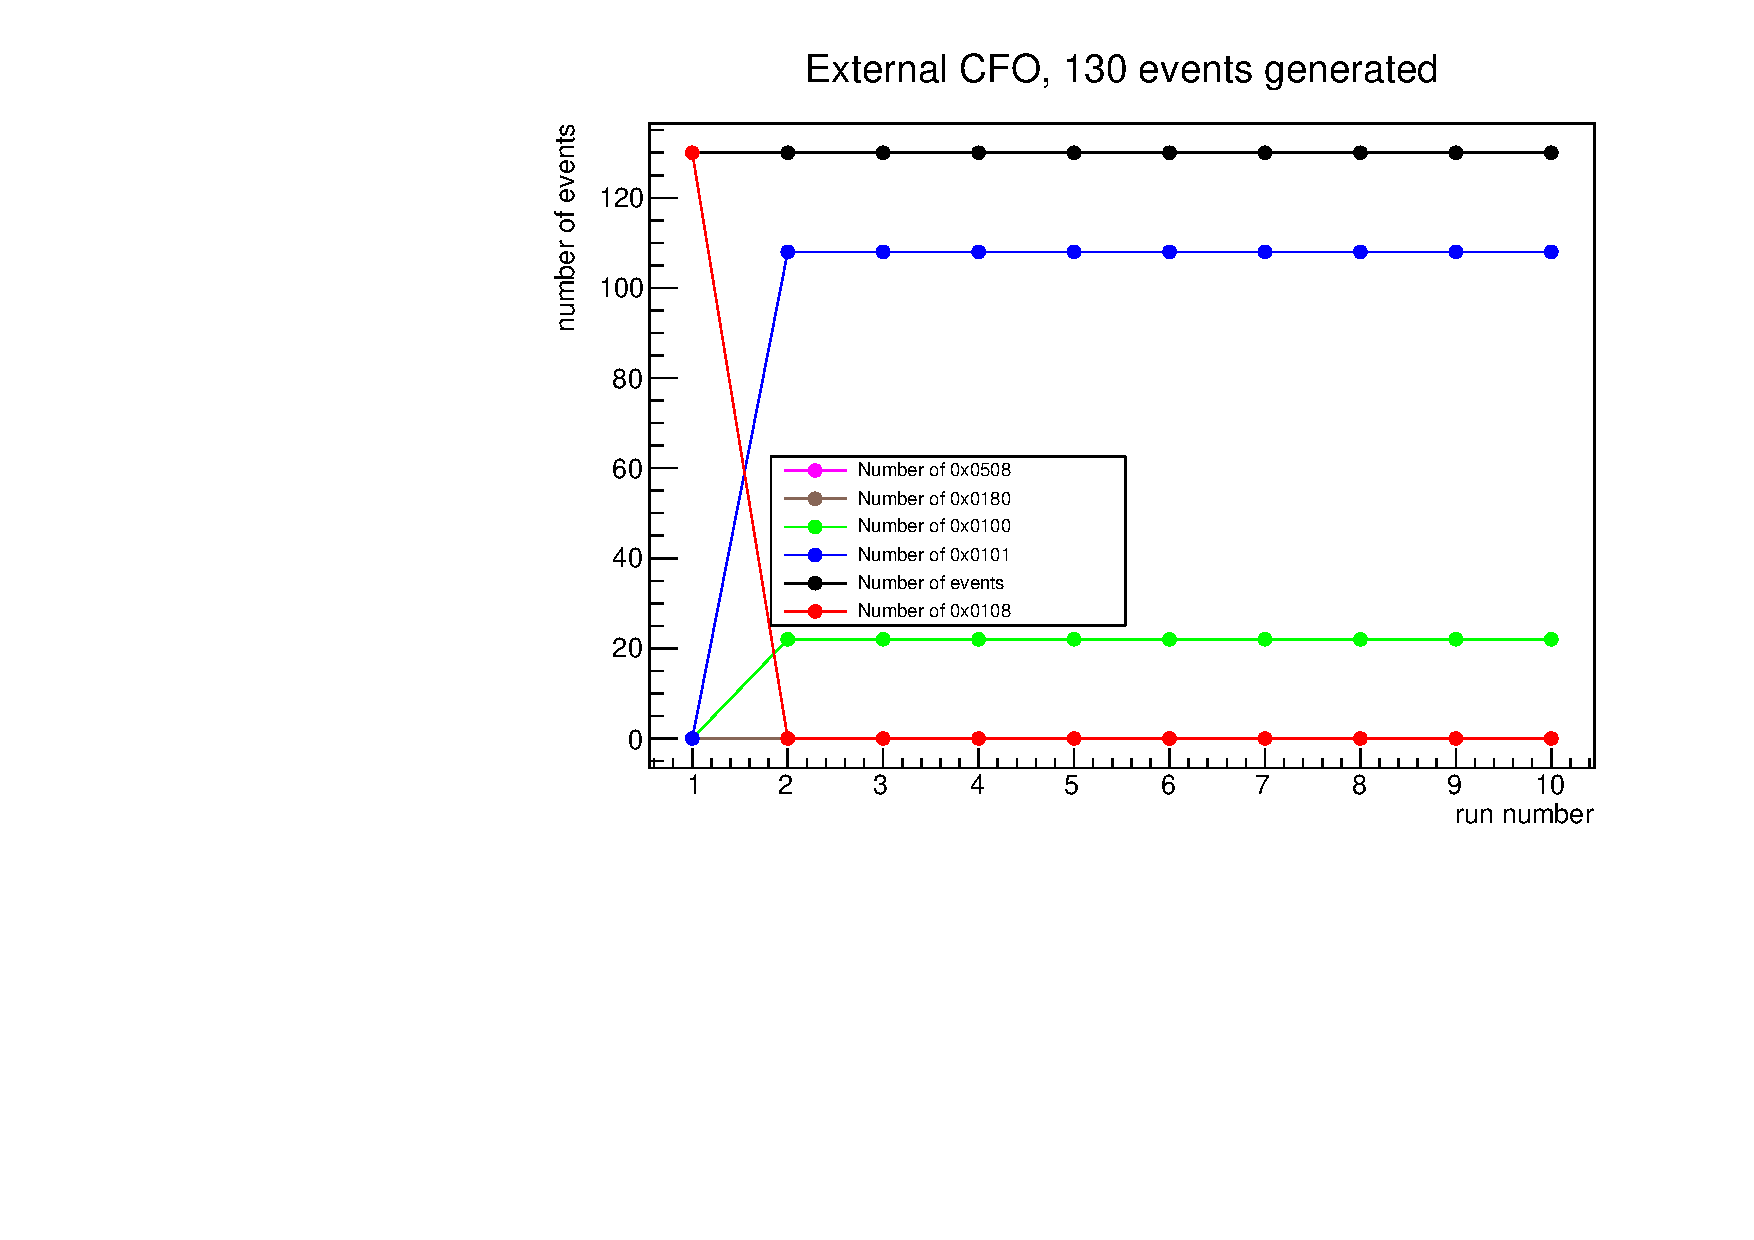
\includegraphics[width=1.1\textwidth]{figures/pdf/130.pdf}
      \caption{}
  \end{subfigure}
  ~ 
  \begin{subfigure}[t]{0.5\textwidth}
    \centering
    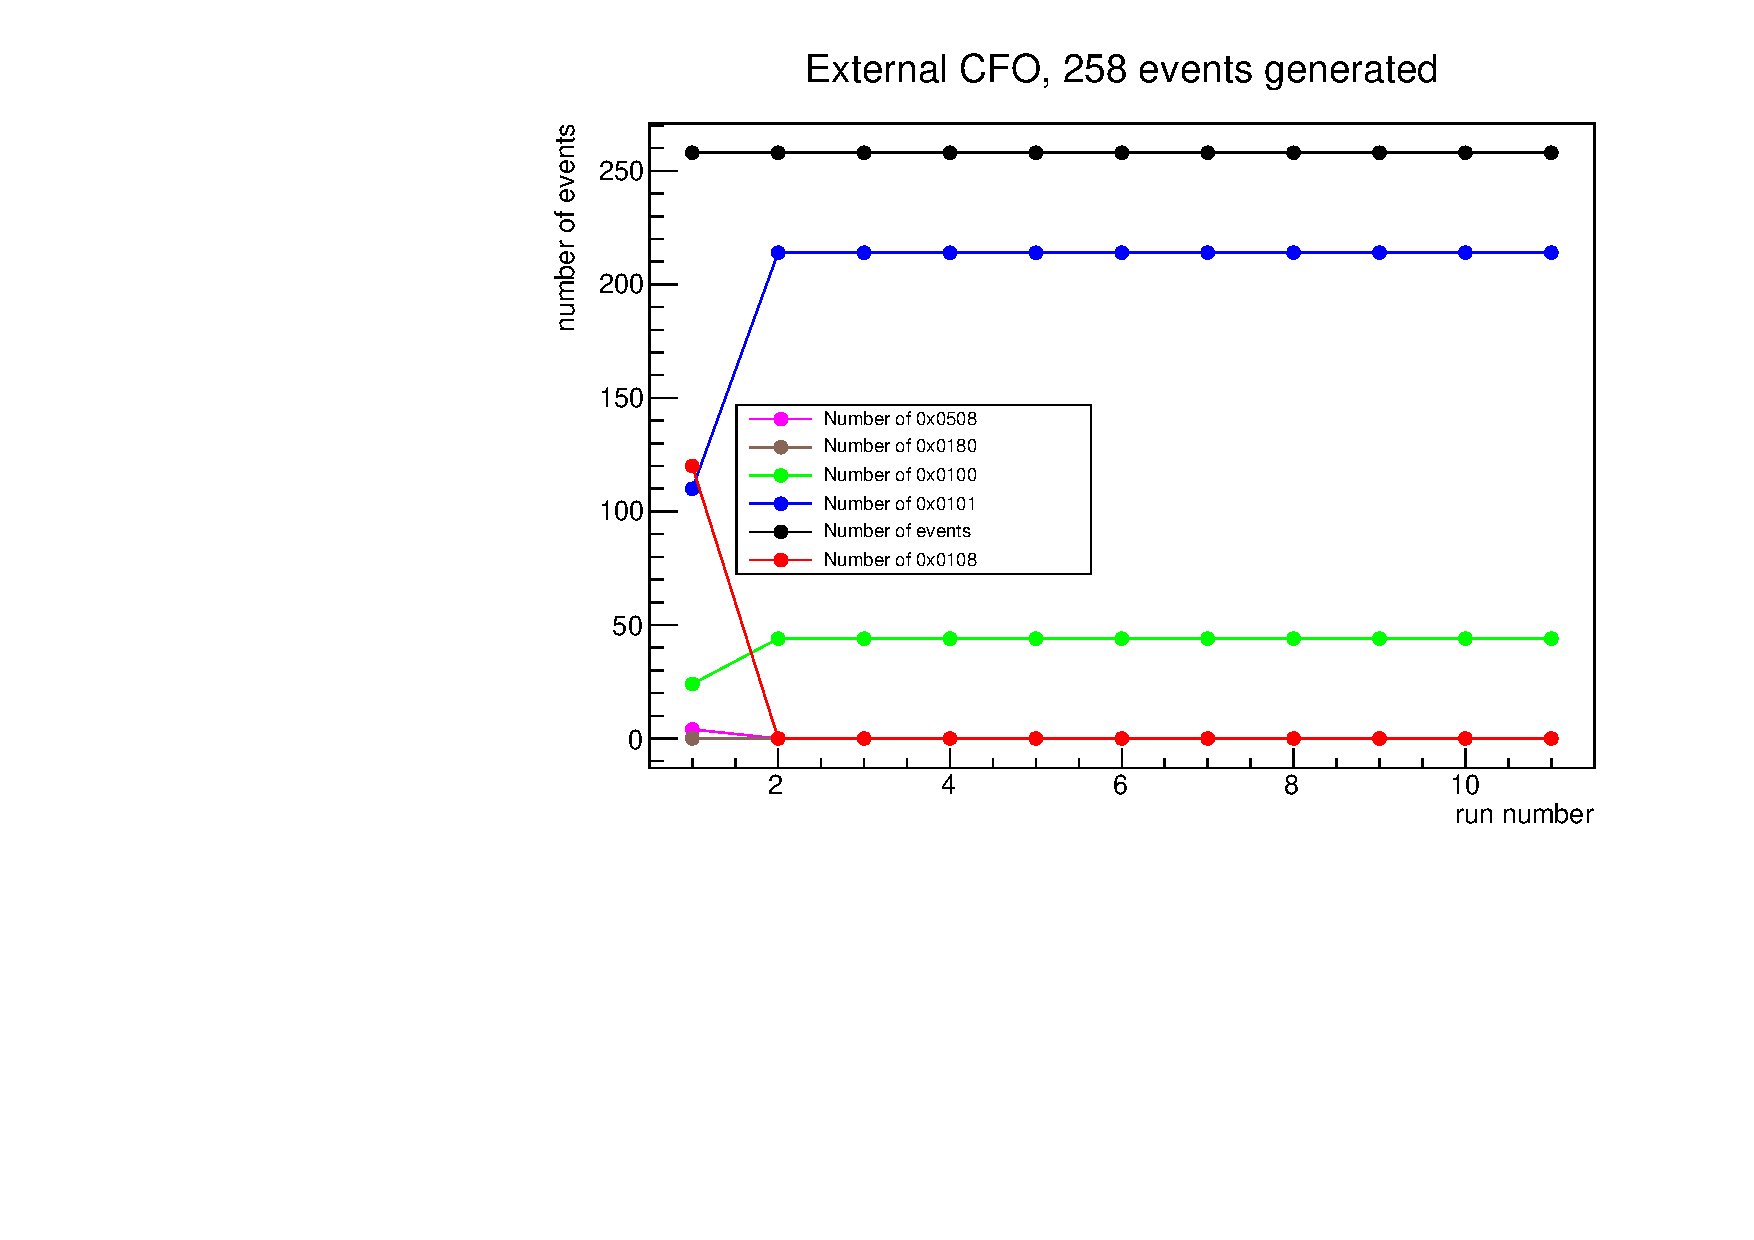
\includegraphics[width=1.1\textwidth]{figures/pdf/258.pdf}
    \caption{}
\end{subfigure}%
~ 
\begin{subfigure}[t]{0.5\textwidth}
    \centering
    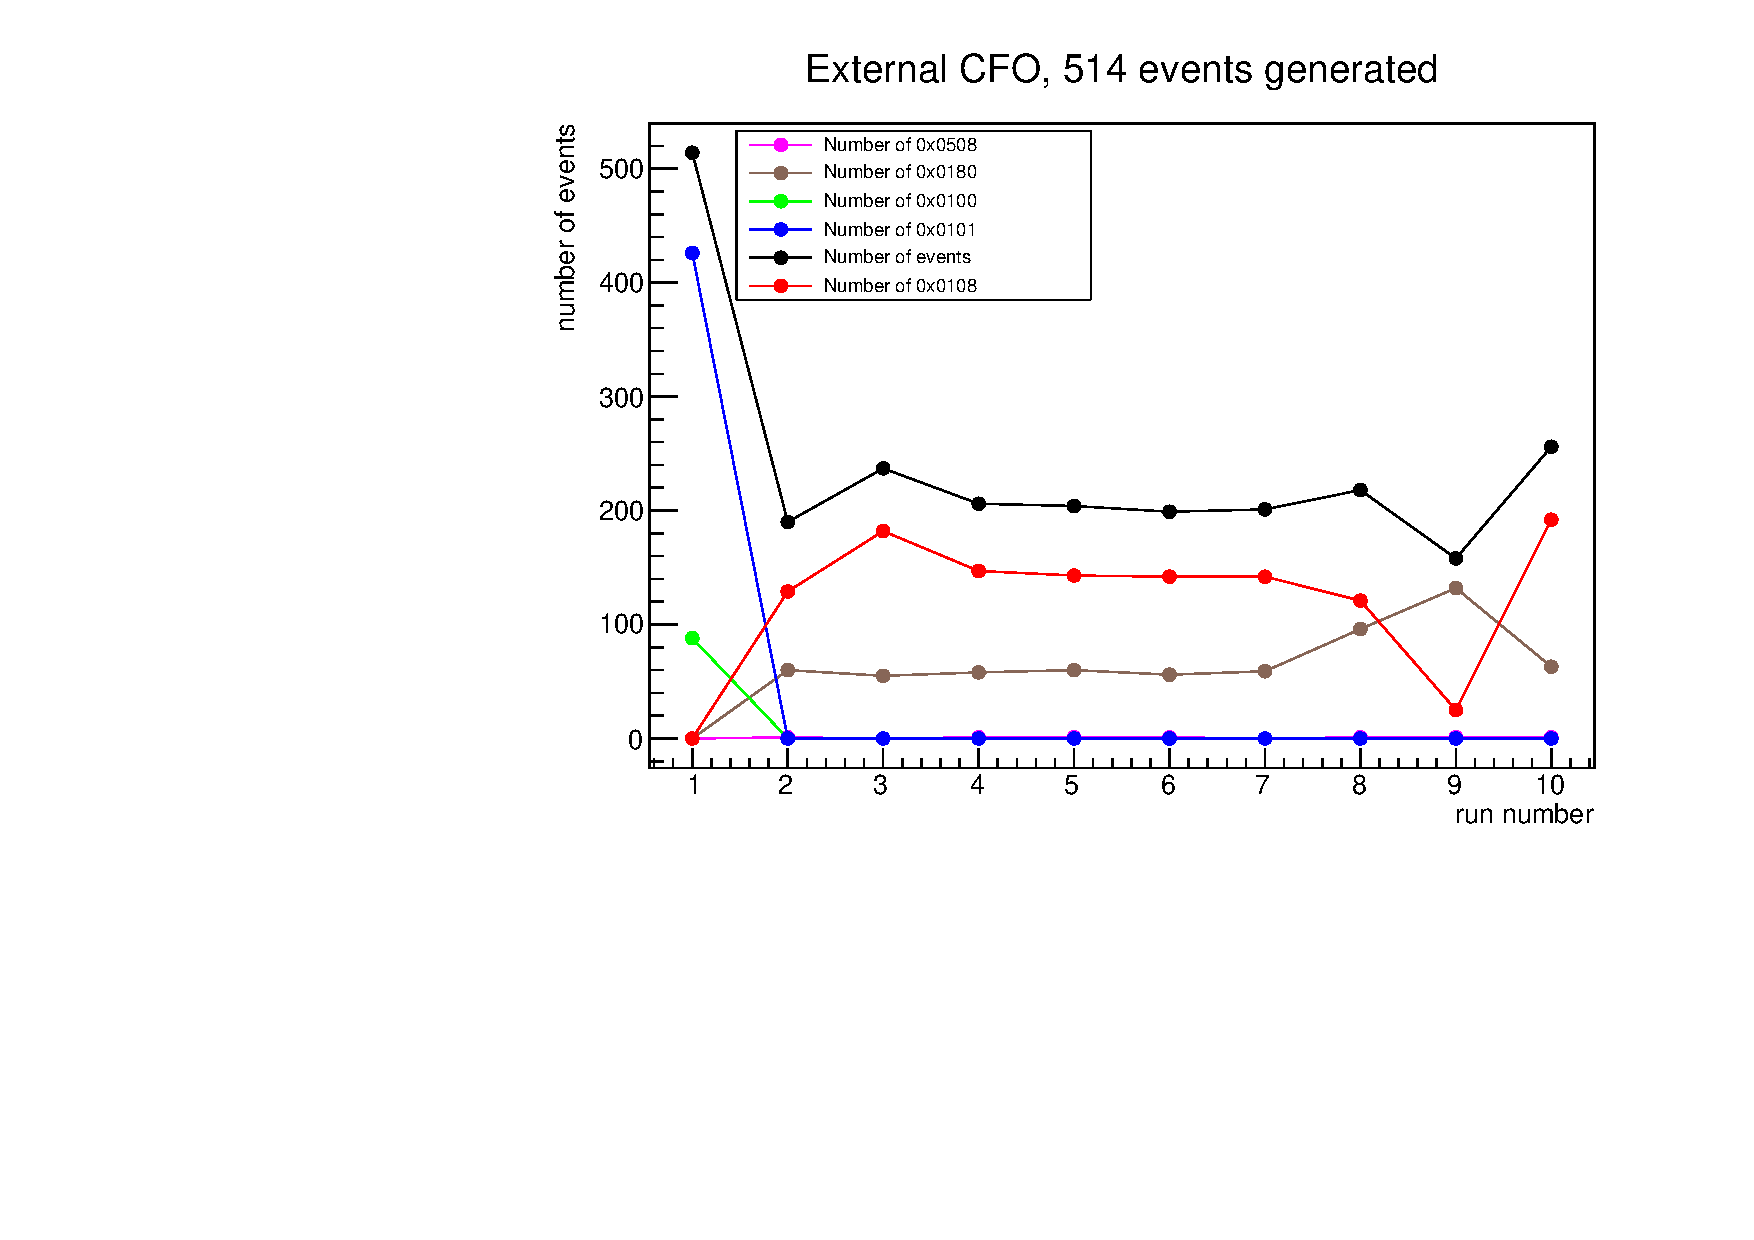
\includegraphics[width=1.1\textwidth]{figures/pdf/514.pdf}
    \caption{}
\end{subfigure}
~ 
\begin{subfigure}[t]{0.5\textwidth}
    \centering
    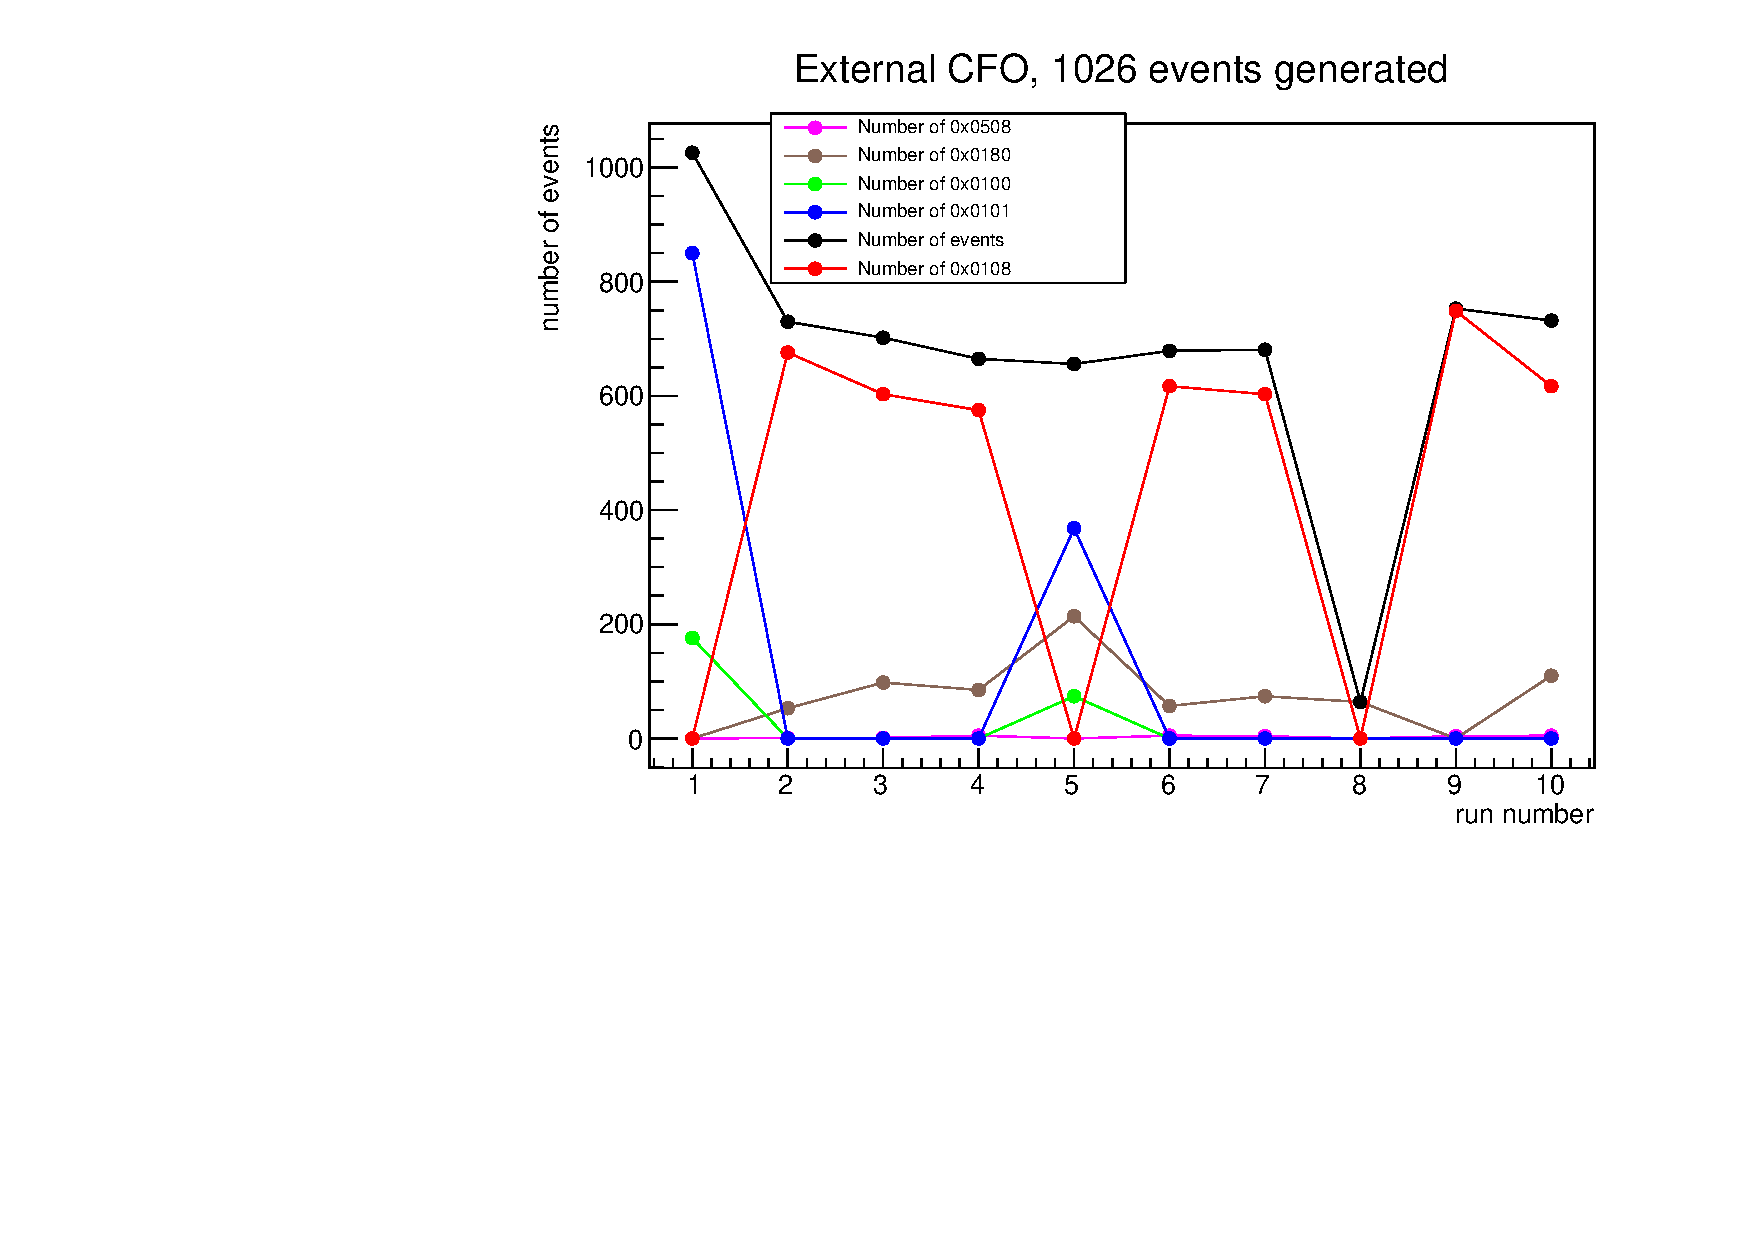
\includegraphics[width=1.1\textwidth]{figures/pdf/1026.pdf}
    \caption{}
\end{subfigure}
  \caption{The  $external \ CFO$ mode. Subfigures (a), (b), (c), (d), (e) show 66, 130, 258, 514 and 1026 events generated respectively. 
  The total number of events (black), the number of empty events (0x100 - green -) and full events (0x101 - blue -), 
  and the number of timeouts (0x108 - red -, 0x180 - brown -, and 0x508 - pink -) versus the run number in a \textit{run plan} are shown.}
  \label{fig:corruption}
\end{figure}



These results have been sent to the firmware developers for further checks.

















\iffalse


\section{High rate software testing}
\subsection{Firmware-Based Data Acquisition}
The Mu2e Trigger and Data Acquisition (TDAQ) system collects digitized data from the Tracker, 
Calorimeter, Cosmic Ray Veto and Beam Monitoring components (Stopping Target Monitor and Extinction Monitor) 
and delivers that data to online and offline processing for analysis. It must merge data from $\sim$450 subsystems 
and apply filters to reduce data volume by a factor of 100 before storing it offline. It is also responsible for 
detector synchronization, control, monitoring and operator interfaces. The Mu2e DAQ system uses a $streaming$ readout technique, 
which means that all detector data from the experiment is digitized and zero-suppressed in their respective Front End Electronics 
(FEEs) before being transferred. This strategy results in a high data flow in the DAQ system while providing greater flexibility in data selection and analysis.
\subsubsection{Expected rate}
The data taking periods will be divided into two modes: on-spill and off-spill. The on-spill mode includes periods when 8 GeV 
proton bunches are colliding with the production target. The off-spill mode includes all other periods, such as between bunches, calibration periods and commissioning.
According to section \ref{accel}, it is possible to estimate the on-spill event contribution as follows:
\begin{itemize}
    \item $\frac{43.1 \text{ ms (time of one spill)}}{1695 \text{ ns (digitization time)}}$ = 25,000 pulses per spill;
    \item 8 (number of spills) $\times$ 25,000 (pulses per spill) = 200,000 on-spill events per cycle;
    \item $\frac{200,000 \text{ (on-spill events per cycle)}}{1.4 \text{ s (cycle time)}}$ = 145,000 on-spill events per second.
\end{itemize}
%di questi 1.4s, 1.055s si riferisce all'offspill e 0.4s all'onspill.
Meanwhile, the off-spill event contribution is:
\begin{itemize}
    \item $145,000 \text{ (on-spill events per second)} \times 0.4 \text{ s (off-spill time)}$ = 58,000 off-spill events per cycle;
    \item $\frac{58,000 \text{ (off-spill events per cycle)}}{1.4 \text{ s (cycle time)}}$ = 41,000 off-spill events per second.
\end{itemize}
The total input rate will be 186,000 events/s. %Hz
There is a mean factor 100 of trigger, so 1800 events/s.
The detectors will generate $\sim$150,000 Byte per event of zero-suppressed data, for an average data rate of $\sim$90 GB/s when beam is present. 
To reduce DAQ bandwidth requirements, this data is buffered in Readout Controller (ROC) memory during the spill period and transmitted to the 
DAQ over the full supercycle for an average data rate of $\sim$28 GB/s.
The total input is 150,000 Byte per event $\times$ 1800 events/s that is 270 MB/s.
\subsection{ARTDAQ}
\section{Data flow testing}
\section{ROC firmware testing}


2214 straw hits per event (DocDB-10898)
- Event = micro bunch (1.6usecs)
 Each hit = 32 bytes (ignores special characters, CRCs…)
 So total 44GB/s
 Assume uniform in z (which is definitely a bad assumption, 6:1
front back asymmetry) this 200MB/s per ROC
\fi

 %(1695 ns), that is 90 GB/s and there is a buffering factor of 0.4/1.4, that makes 28 GB/s.


%In Figure \ref{fig:linktodaq}, the general design of the Mu2e DAQ system is shown.

%The left blocks represent the Readout Controllers (ROCs) in different detectors. The center 
%lock houses the DAQ system's online components, which include the Run Control Host, 40 DAQ servers, 
%the Detector Control System (DCS) and the Event Building Switch. The Run Control Host receives beam status 
%and timing information from the Accelerator Controls network and operator commands from the remote control room. 
%The Detector Control System (DCS) is the window onto the status and health of the Mu2e detector. The Event Building 
%(EVB) function combines these subsets to form a complete detector data set for analysis by an online processor, Ref. 
%\cite{bartoszek2015mu2e}. Event building is typically done in a switching network to sustain high rates. The right block 
%houses the DAQ system's offline components, which are $\mu$sed for data storage and processing. During an active spill 
%(the first approximately 43 ms of the 48 ms bunch extraction cycle outlined in Chapter \ref{accel}), the experiment receives
% RF Zero-Crossing Markers from the Accelerator that are synchronized to the 1695 ns proton pulse cycles (the event windows). 
% Based on these markers, the Command Fan-Out (CFO) module within the Run Control Host generates a 40 MHz system clock and encodes 
% Event Window Markers (EWMs) in the system clock to indicate the start of the event windows. The CFO then sends the encoded system 
% clock, along with run control packets, to Data Transfer Controllers (DTCs) in the DAQ servers. The DTCs\footnote{The Mu2e Data 
% Transfer Controller (DTC), Ref. \cite{ryan} takes data from various Read-Out Controllers and may conduct event construction and 
% data preprocessing. The DTC module connects a maximum of six ROCs to the Trigger and Data Acquisition (TDAQ) servers, 
% which execute the TDAQ online software framework.} then transfer the encoded clock to the detectors' ROCs, where the EWMs 
% are recovered with fixed delay relative to the original RF Zero-Crossing Markers and $\mu$sed in the local ROCs to discriminate 
% data acquired during consecutive event windows. The Tracker generates a DDR3 memory address at the beginning of each event window. 
% The relevant memory area is designated to hold Tracker hits received during that event window. Data requests trigger data readouts 
% from the ROCs to the DAQ system. The Data Requests are modifiable through the CFO as described by the Run Plan, although they are 
% initially given to the Tracker and Calorimeter ROCs via the DTCs following each event window.
% Each tracker hit is composed of a data packet having a fixed length of 128 bits (16 bytes):
 %\begin{itemize}
  %   \item 16 bit header - it contains information as a packet header, a channel identifier to 
   %  specify the channel so the ROC can assign the hit to a wire number and a packet checksum;
    % \item 16 bit - TDC left straw end;
    % \item 16 bit - TDC right straw end;
    % \item 8$\times$10 bit ADC.
% \end{itemize}






%A packet of 128 bits can be transferred every 640 ns (200 Mbps).An additional 32
%bits must be added as an end-of-file marker after the data $\mu$spill hit data is buffered.
%The ROC-to-DAQ connection is made via fiber optic links arranged in rings, with multiple ROC per ring, as shown in Figure \ref{fig:linktodaq}. 
%This is possible since a single optical link can handle 2.6 Gbps, while the ROC output is around 230 Mbps. This value comes from the fact that the 
%highest rate for any 4 straws group (corresponding to one digitizer data line to the ROC) is 240 kHz or 30 Mbps (at 128 bits/hit) and the Main Injector 
%supplies Mu2e beam only 32\% of the time. The ROC monitors slow control variables and controls panel operations too.


